% basically this is a template file, you should be able to take it and
% start running.

% the philosophy behind this template is that each chapter or
% chapterlike section goes in a separate file and you use the \include
% command to input it into the final document.  The \includeonly
% command can be used so you only need to work on one or two chapters at a
% time (instead of having to either latex the entire book each time or
% losing cross-references and page numbering)

% copy this file and call it something like mythesis.tex

\documentclass[10pt]{report}
% note that the documentclass can take other option such as
% twoside - for double sided printing
% openright - if double side  chapters always start on odd pages
% openany - if double side chapters start on the next page even or odd
% 12pt can be replaced by 11pt

\usepackage{suthesis-2e}
% options are
% online - now the default
% hardcopy - turns off online includes signature page and copyright page in file 
% engineer - does an engineer thesis instead of a PhD dissertation

%% load other packages you need

%% uncomment the following and create mythesis-macros.sty for all your
%% own macros.  This keeps this top level file looking fairly neat.
% \usepackage{mythesis-macros}

%% certain types of theses require special title page format.  See the
%% style file for the full list.  An example would be that for some of
%% the language departments. 
% \dualthesis \dept{Asian Languages} \languagemajor{Korean} 
%% or education
% \educationthesis

\title{Scaling a Reconfigurable Dataflow Accelerator}
\author{Yaqi Zhang}
\dept{Electrical Engineering} % default is Computer Science, uncomment for other departments
\principaladviser{Kunle Olukotun}
% \coprincipaladvisor{}
\firstreader{Subhasish Mitra}
\secondreader{Matei Zaharia}
% \thirdreader{}

%the following command would (if uncommented) allow  only chapter1 and
%chapter2 to be processed
%\includeonly{chapter1,chapter2}

% if you feel real savvy use
% \typein{Now put in includeonly}
% the \typein command stops latex at this point and allows you to type
% in a command such as
% \includeonly{chapter3,chapter5}
% this can save some time and means you don't have to edit this file
% as much.

\usepackage[T1]{fontenc}

%% Font of document
\usepackage{tgpagella}
%\usepackage{tgbonum} %% no good
%\usepackage{bookman} %% no good
%\usepackage{charter} 
%\usepackage{courier} 
%\usepackage{mathptmx}
\renewcommand{\baselinestretch}{1.5}

\usepackage{graphicx}

\usepackage{listings}           % Code listing
\usepackage{courier}
\usepackage{xcolor}
\definecolor{vbgray}{gray}{0.9}
\definecolor{darkgreen}{RGB} {0, 100, 0}
\definecolor{darkred}{RGB} {255, 0, 0}
\def\tick{{\color{darkgreen} \textbf{\tikz\fill[scale=0.5](0,.35) -- (.25,0) -- (1,.7) -- (.25,.15) -- cycle;}}}
\def\ytick{{\color{orange} \textbf{\tikz\fill[scale=0.5](0,.35) -- (.25,0) -- (1,.7) -- (.25,.15) -- cycle;}}}
\def\x{{\color{darkred} {$\bm{\times}$}}}

\definecolor{red}{RGB}{255,0,0}
\definecolor{vbgray}{gray}{0.9}
\definecolor{darkgreen}{RGB} {0, 100, 0}
\definecolor{darkred}{RGB} {255, 0, 0}
\definecolor{blue}{RGB} {0, 135, 255}
\definecolor{yellow}{RGB} {224, 173, 0}
\definecolor{codegreen}{RGB}{52,123,0}
\definecolor{codegray}{rgb}{0.6,0.5,0.5}
\definecolor{codepurple}{rgb}{0.58,0,0.82}
\definecolor{backcolour}{rgb}{0.97,0.97,0.97}
\definecolor{lightback}{rgb}{0.95,0.95,0.95}
\def\tick{{\color{darkgreen} \textbf{\tikz\fill[scale=0.5](0,.35) -- (.25,0) -- (1,.7) -- (.25,.15) -- cycle;}}}
\def\ytick{{\color{orange} \textbf{\tikz\fill[scale=0.5](0,.35) -- (.25,0) -- (1,.7) -- (.25,.15) -- cycle;}}}
\def\x{{\color{darkred} {$\bm{\times}$}}}

\lstdefinelanguage{Spatial}{
  basicstyle=\fontsize{7}{7}\selectfont\ttfamily,frame=tlbr,framesep=4pt,framerule=0pt,
  tabsize=2,
  basewidth={0.55em, 0.4em},%
  numbers=left,
  showspaces=false,  
  keywordstyle=\bfseries,   
  breaklines=true,
  columns=fixed,
  %xleftmargin=0.25in, 
  firstnumber=auto,
  showstringspaces=false,
  escapechar=@,
  escapeinside={(*@}{@*)},
  morestring=[b]",
  morestring=[b]',
  morecomment=[l]{//},
  morecomment=[s]{/*}{*/},
  backgroundcolor=\color{backcolour},   
  commentstyle=\color{codegreen}, %\bfseries,
  numberstyle=\tiny\color{codegray},
  stringstyle=\color{codepurple},
  keywordstyle=[2]\color{blue},
  keywords=[2]{val, def, type},
  keywordstyle=[3]\color{yellow}\bfseries,
  keywords=[3]{Float, Int, String, T, Void, Bit, Half, FltPt},
  keywordstyle=[4]\color{orange}\bfseries,
  keywords=[4]{Matrix, Array},
  keywordstyle=[5]\color{blue}\bfseries,
  keywords=[5]{StreamIn, StreamOut, DRAM, ArgIn, ArgOut, HostIO, RegFile, Reg, SRAM, FIFO, LIFO, LUT, LineBuffer},
  keywordstyle=[6]\bfseries,
  keywords=[6]{enq, deq, load, store, scatter, gather, :=, value, push, pop, peek},
  keywordstyle=[7]\color{magenta},
  keywords=[7]{until, par, by},
  keywordstyle=[8]\color{red}\bfseries,
  keywords=[8]{C0,C1,C2,C3,C4,C5,C6,C7,C8,C9,C10},
  keywordstyle=\color{magenta}\bfseries,
  morekeywords={Foreach,Reduce,MemReduce,MemFold,Fold,Accel,Stream,FSM,Sequential,if,else,Parallel,Pipe, DummyPipe}
}


\usepackage{outlines}
\usepackage{booktabs}
\usepackage{multirow}
%\usepackage[numbers,sort&compress]{natbib}
\usepackage{amsmath}
\usepackage{amsfonts}
\usepackage{siunitx}

\usepackage{makecell}

%% Code formatting
\usepackage{minted}

%% To enable sub figures
\usepackage{caption}
\usepackage{subcaption}

\usepackage{algorithm2e}
\SetStartEndCondition{ }{}{}%
\SetKwProg{Fn}{Function}{\string:}{}
%\SetKwProg{Fn}{}{}{}
\SetKw{KwTo}{in}
\SetKw{KwNew}{new}
\SetKwIF{If}{ElseIf}{Else}{if}{:}{elif}{else:}{}%
\SetKwFor{For}{for}{\string:}{}%
\SetKwFor{While}{while}{:}{}%
\AlgoDontDisplayBlockMarkers%
\SetAlgoNoEnd%
\SetAlgoNoLine%
\SetKwFunction{Range}{range}%%

\usepackage[hidelinks]{hyperref}
\usepackage[capitalise]{cleveref}
\usepackage{xspace} 
\usepackage{todonotes}

\setminted[python]{linenos, frame=lines, framesep=2mm, baselinestretch=0.8, fontsize=\footnotesize,escapeinside=||}
%\usemintedstyle{pastie}

\newcommand{\name}{SARA\xspace}
\newcommand{\rda}{RDA\xspace}
\newcommand{\rdas}{RDAs\xspace}
\newcommand{\gist}[1]{{\color{blue} #1}}
\renewcommand{\todo}[1]{{\color{red} TODO: #1}}
\newcommand{\term}[1]{\textbf{#1}}
\newcommand{\eg}{{\em e.g.}}
\newcommand{\CL}[1]{\textbf{\textcolor{red}{#1}}}
\definecolor{brightpurple}{RGB}{163,33,247}
\newcommand{\CK}[1]{\textbf{\textcolor{brightpurple}{#1}}}

\usepackage{pifont}
\newcommand{\cmark}{\textcolor{green!80!black}{\ding{51}}}
\newcommand{\xmark}{\textcolor{red}{\ding{55}}}
%\newcommand{\cmark}{\ding{51}}
%\newcommand{\xmark}{\ding{55}}

%%
%% Math operators
\DeclareMathOperator*{\argmax}{argmax}
\DeclareMathOperator*{\elmax}{elmax} % Elementwise maximum
\DeclareMathOperator*{\dest}{dest} % Destinations for an operator (its consumers)
\DeclareMathOperator*{\andf}{and}
\DeclareMathOperator*{\maximum}{maximum}

\newcommand{\projb}[1]{\text{proj}_\mathbf{B}(#1)}
\newcommand{\nnint}{\mathbb{Z}_{\ge 0}}
\newcommand{\ind}[1]{\mathbb{1}[#1]}


\begin{document}

% first the preface sections.  

% this includes the file preface.tex which should include the
% following commands
% \beforepreface
% \prefacesection{preface}
% body of the preface

\beforepreface

\prefacesection{Abstract}

With the slowdown of Moore’s Law, specialized hardware accelerators are gaining traction for delivering 100-1000x performance improvement over general-purpose processors in a variety of applications domains, such as cloud computing, biocomputing, 
artificial intelligence, etc.~\cite{fpgacloudsurvey,bioaccel,genomicaccel}.
As the performance scaling in multicores is coming to a limit~\cite{multicorescale}, a new class of accelerators--reconfigurable dataflow architectures (RDAs)--offers a promising high-throughput and energy-efficient acceleration that keeps up with the performance demand.
Instead of dynamically fetching instructions like in traditional processors, RDAs have flexible datapath  that can be statically configured to spatially parallelize and pipeline the program across
distributed on-chip resources. 
The pipelined execution model and explicitly-managed scratchpad in RDAs eliminate the performance, area, and energy overhead in dynamic scheduling and a conventional memory hierarchy.

To adapt to the compute intensity in modern data-analytic workloads, particularly in the deep learning domain, RDAs are increasing to a scale that was unprecedented before.
With an area footprint of $133\text{mm}^2$ at 28nm, 
Plasticine is a large-scale RDA supplying 12.3 TFLOPs of computing power~\cite{plasticine}.
Prior work has shown an up to 76x performance/watt benefit from Plasticine over a Stradix V FPGA 
due to an advantage in clock frequency and resource density.
The increase in scale introduces new challenges in network-on-chip design to maintain 
the throughput and energy efficiency of an RDA.
Furthermore, targeting and managing RDAs at this scale require new strategies in mapping,  memory management, and flexible control to fully utilize their compute power. 

In this work, we focus on two aspects of the software-hardware co-design that impact the usability
and scalability of the Plasticine accelerator. 
Although RDAs are flexible to support a wide range of applications, 
the largest challenge that hinders the adoption of these accelerators is 
the required low-level knowledge in microarchitecture design and hardware constraints in
order to efficiently map a new application.
To address this challenge, we introduce a compiler stack--\name--that raises the programming abstraction of
Plasticine to an imperative-style domain-specific language with nested control
flow for general spatial architectures.
Besides architecture-agnostic, this abstraction contains explicit loop constructs, enabling
cross-kernel optimizations that are often not exploited when programming RDAs.
\name efficiently translates imperative control constructs to a streaming
dataflow graph that scale performance with distributed on-chip resources.
By virtualizing resources, \name systematically handles the physical constraints, hiding
the low-level physical limitations from programmers.
To address the scalability challenge with increasing chip size, 
we present a comprehensive study on the network-on-chip design space for RDAs~\cite{network}.
We found that network performance highly correlates to bandwidth, as supposed to latency,
for RDAs with streaming dataflow execution model.
Lastly, we show that a static-dynamic hybrid network design can sustain performance in a 
scalable fashion with high energy efficiency.

\prefacesection{Acknowledgements}

As a start, I would like to thank the most impactful person in my graduate adventure--my advisor
Kunle Olukotun.
Retrospectively, Kunle provided many constructive suggestions that set forth a good foundation for my research.
While Kunle knows what is right, he allows us to explore and make mistakes.
A frequent question from Kunle during our one-on-ones is ``So, what's the plan?'.
One of the most valuable skills I have acquired from graduate school beyond the technical expertise is the ability to construct an executable plan for a new problem, realize the defects in the initial solution, and persistently refine the implementation, which results in innovations.

Many other Stanford professors have benefited my research from various perspectives.
I would like to thank Subhasish Mitra and Christos Kozyrakis for their past support on the
Plasticine project.
Interactions with Matei Zaharia and Chris R\'e during DAWN retreats also enlarged my scope on 
software advancement in machine learning research and frameworks.
I would also like to thank Juan Rivas to join my defense as my committee chair and evaluating the
contribution of the work for a broader audience.

I have encountered a group of exceptional colleagues at Stanford and
benefited tremendously in my professional skills\footnote{and other random knowledge} during interactions with my peers.
David Koeplinger answered many of my Scala questions and I have learned a great deal about compiler
infrastructures by reading his code.
Raghu Prabhakar had always been extremely helpful and instrumental in research discussions. 
He often put himself in others' shoes that he was always the most popular person on the planet back at school and now at work.
Alex Rucker made a great contribution to Plasticine's network design and introduced a high-level simulator that relieved me from RTL simulation, which undoubtedly expedited my graduation.
Matt Feldman enhanced the Spatial compiler and made it robust, which supported the research of mine and many
others, both inside and outside our group.
Matt also contributed his dog, Daisy, to befriend with everyone and 
provide de-stress after a hard-working Friday afternoon.
Tian Zhao provided generous support on experiment setup and baseline collections during many of my paper deadlines.
I had a great collaboration experience with Matt Vilim, who also introduced me to ergonomic keyboards.
Nathan Zhang contributed considerably to solver-related works and was always the happiest person in the group that positively affected everyone.
Muhammad Shahbaz was particularly helpful on paper editing and helped me identify the impact and contribution of my work.
I had a fun cross-domain collaboration with Rekha Singhal and Jeff Ullman to design new algorithms for our
hardware.

I would also like to thank everyone in Kunle's group and all of the DAWN members, including but not limited to, 
Tushar Swamy, Olivia Hsu, and Luigi Nardi. 
All of you are an important part of my graduate school experience.
I appreciate the hard work our Admins--Dan Moreau and Andrea Brand-Sanchez--had put forth that
offered us a smooth experience for graduate school.

I would like to share my gratitude towards my undergraduate research advisor, Daniel J. Sorin, who has taught the
majority of my architecture classes and inspired my research interests in this area.
I would not have experienced such a fruitful journey and acquainted so many outstanding people
without his mentoring and encouragement.

Last but not least, I would like to thank my friends and family for continuous support during my
graduate school. 
Friends have always been my first source for help ever since I left home and studied abroad.
They have enriched my life beyond research, making the past five years both enjoyable and
unforgettable.
My parents' passion for research has always inspired me to pursue a Ph.D., and their encouragement and
acknowledgments equipped me with tremendous strength and confidence to complete this adventure.
Finally, I would like to thank my boyfriend, Charles, for always by my side during the happiest and the most stressful moments. 
He was especially understanding and supportive that he would
share my household burden during deadlines and accommodate my irregular sleeping and working schedules.
My graduate school journey would be much more challenging and less rewarded without the support from all these people.


%% afterpreface produces a table of contents and any other tables
%% wanted. At the end pagenumbering changes from roman to arabic and
%% is restarted
\afterpreface

\chapter{Introduction (WIP)}

\section{The Rising of Hardware Acceleration}

With the end of Dennard Scaling~\cite{dennard}, the amount of performance one can extract from a CPU is reaching a limit.
To provide general-purpose flexibility, CPUs spend the majority of resources and energy on overheads, 
including dynamic-instruction fetching and decoding, branch prediction, and a cache hierarchy, etc., 
with less than 20\% of 
the energy on the actual computation~\cite{mark}.
Even worse, power wall is limiting the entire multicore family
to reach the doubled performance per generation enabled by technology scaling in the 
past~\cite{multicorescale}.

For this reason, hardware acceleration is emerging in various compute-intensive application domains 
to provide orders of magnitude acceleration, enabling algorithms that were otherwise
infeasible~\cite{genomicaccel, bioaccel, fpgadeeplearn, fpgacripto}.
Examples include widely adopted General-Purpose Graphics Processing Units (GPGPUs) 
in computational genomics, signal processing, graph processing, and
deep learning, etc.~\cite{genomicaccel, bioaccel, fpgacloudsurvey}.
Moreover, many recent efforts are spent on leveraging application domain knowledge in hardware design to enable 
continued performance scaling while meeting the power budget~\cite{turinglecture}.
As artificial intelligence receiving great success in industry and business,
past years have seen a growing interest in machine learning accelerators;
these accelerators contain specialized circuits for ML kernels that dramatically improve the compute
efficiency~\cite{dadiannao,tpu,eie,chen2017eyeriss,tangram,truenorth}.

Nonetheless, it is non-trivial to achieve good utilization of these accelerators.
While the peak FLOPS of GPU has increased by over 20x in the past 10 years, the achievable FLOPS is
not increasing accordingly~\cite{floptrend, gpuperfana}.
The massive threads in GPU require embarrassedly parallel workloads to fully saturate the compute
throughput. GPU's bulk-synchronous nature also causes poor cache efficiency; data are spilled
off-chip before getting reused~\cite{gpuinefficiency}.
On the outer hand, 
while extremely efficient for certain models, machine learning accelerators are highly
specialized for specific kernels, especially general matrix multiply (GEMM) and convolution.
However, ML algorithms evolve much faster than the development and manufacture cycle of hardware, 
leading to inefficiency or even unsupported applications.
For example, hybrid models, such as Mask R-CNN~\cite{maskrcnn} and DeepLab~\cite{deeplab}, contain
combinations of GEMM-compatible and incompatible operations, both computationally expensive.
Fix-functional accelerators focusing on GEMM operations, such as TPU~\cite{tpu}, 
have to rely on CPUs for unsupported operations or
convert non-GEMM operations to GEMM operations, resulting in a severe performance gap between the
peak and effective FLOPS~\cite{effflexdnnaccel}.
\Cref{fig:peakutil} illustrate a tradeoff between average utilization of the peak FLOPS over a range
of data and the peak FLOPS available on the hardware.

\begin{figure*}
\centering
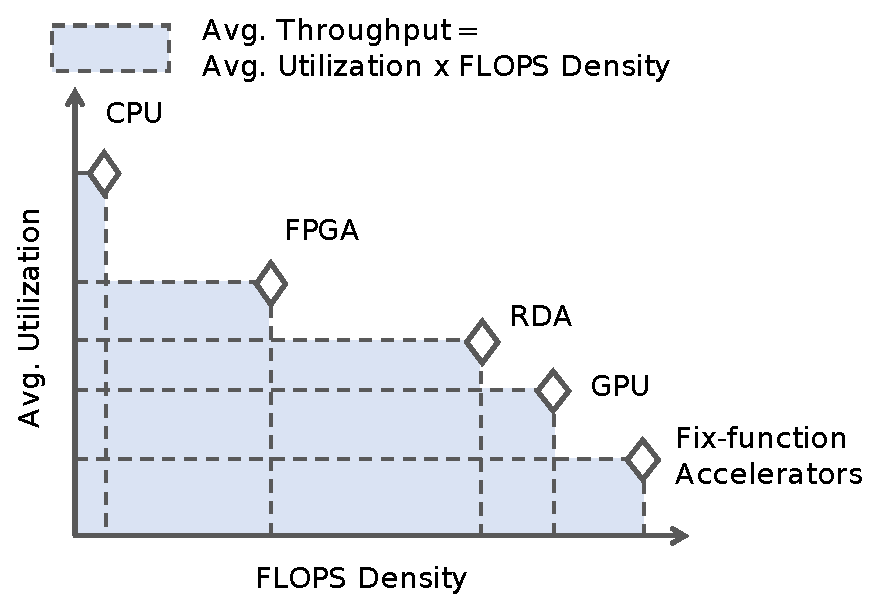
\includegraphics[width=0.4\textwidth]{figs/peakutil.pdf}
\caption[Average utilization vs. peak compute density tradeoff]{
 Tradeoff between the average utilization of the peak FLOPS over a range of applications vs. the peak compute density 
 among different architectures.
 The shaded area indicates the effective FLOPS achieved.
 With all the dynamic scheduling hardware in CPUs, such as prefetching and branch prediction, 
 CPU can achieve a fairly decent instruction per cycle (IPC) for data-analytic workloads that have a 
 regular control flow. 
 However, overheads to support flexibility, security, and programmability in CPU result in a low FLOPS
 density. 
 While GPU and fix-function accelerators have a high FLOPS density, they are prone to
 underutilization due to variation in application characteristics. 
 Fine-grained reconfigurable datapath makes it easy to utilize on-chip resources of an FPGA.
 However, the soft logics and overheads in routing resources lead to a low resource density and clock frequency.
 RDAs have the right balance between flexibility and efficiency, which gives a good overall average utilization.
}
\label{fig:peakutil}
\end{figure*}

Reconfigurable spatial architectures overcome this limitation by changing its datapath based on applications' needs.
Applications are configured at the circuit-level without dynamic instruction fetching and decoding,
hence improving energy-efficiency~\cite{calhoun,fpgaPower}.
In addition to instruction, data, and task-level parallelism explored by processor architectures, spatial architectures also explore instruction and task-level
pipelining that further increase the compute throughput~\cite{spatial-computation}.
Exploring pipeline parallelism enables spatial architectures to achieve a high-throughput
without massively parallelize every stage of the program.
Flexible datapath also permits resource distribution proportional to the compute intensity of
program stages.
A key performance optimization on reconfigurable accelerators is an application-level design space
exploration 
searching for the best resource distribution scheme that balances the compute pipeline~\cite{dse_koeplinger}.

One of the mainstream reconfigurable spatial architecture is 
Field Programmable Gate Arrays (FPGAs) that support fine-grain, 
bit-level reconfigurability with a soft logic fabric~\cite{fpga-survey}.
The flexible interconnect and lookup table-based logic gate can be configured to implement arbitrary
datapath.
FPGAs have been used to deploy services commercially~\cite{microsoft, baidu, deephi} and can be rented on the AWS F1 cloud~\cite{aws}. 
Although around for a long time, FPGAs are not broadly accepted among high-level application programmers due to their low-level programming interface and long compilation time.
Fine-tuning applications on FPGAs require expertise in digital design and takes a long
development cycle, which hinders their accessibility to the general software community.
As an application-level accelerator, FPGAs also suffers from overhead in fine-grained reconfigurability; 
studies have shown that over 60\% of the chip area of an FPGA is spent on routing resources~\cite{fpgaSurvey, calhoun, fpgaPower}. 

%Lately, Reconfigurable Dataflow Architecture (RDAs)~\cite{plasticine, ti, streamdataflow,neuflow,cnndataflow,dataflowarch} are emerging as a new class of spatial accelerators that 
%retain the desired level of flexibility and energy efficiency without 
%the area overhead and low clock frequency due to bit-level reconfigurability.
%As a subclass of Coarse-Grained Reconfigurable Arrays (CGRAs), RDAs also have
%coarse-grained building blocks, such as ALUs, register files, and memory controllers, 
%distributed in a programmable, word or vector-level static interconnect~\cite{adres, kress, dyser, 
%piperench, tartan, hrl, hycube}.

In contrast to fine-grained reconfigurable architectures,
Coarse-Grained Reconfigurable Arrays (CGRAs) are spatial architectures with 
coarse-grained building blocks, such as ALUs, register files, and memory controllers, 
distributed in a programmable, word or vector-level static interconnect~\cite{adres, kress, dyser, piperench, tartan, 
hrl, hycube}.
We refer a subclass of CGRAs with dataflow-driven execution model as Reconfigurable Dataflow
Architectures (RDAs)\footnote{Dataflow overlay architectures on FPGA are technically also RDAs, which are not the primary concern in the discussion of this work.}~\cite{plasticine, ti, streamdataflow,neuflow,cnndataflow,dataflowarch}.
Lately, RDAs are emerging as a new class of spatial accelerators that retain the desired level of
flexibility and energy efficiency without the area overhead and low clock frequency of bit-level reconfigurability.
Our previously proposed RDA--Plasticine--has demonstrated a promising acceleration of dense, sparse, database, and streaming applications~~\cite{plasticine, gorgon, multijoin,prabhakarthesis}.
To meet the computing demand of recent data-analytic workload, Plasticine is a large-scale RDA
compared to traditional CGRAs. 
\Cref{tab:ops} shows the OPS comparison across a few CGRAs proposed in the prior works.

\begin{table}
  \centering
\begin{tabular*}{0.88\textwidth}{cccccc}
  \toprule
  \textbf{Architectures} & DySER~\cite{dyser} & TI~\cite{ti} & revel~\cite{revel}
  & Plasticine~\cite{plasticine} & Gorgon~\cite{gorgon}\\\midrule
  \textbf{OPS} & 128GOPS & 64GOPS & 300GOPS & 12.3TFLOPS & 38.4TFLOPS \\
  \bottomrule
\end{tabular*}
\caption[OPS comparison of different CGRAs]{OPS comparison of different CGRAs. Gorgon is a
Plasticine variant proposed for joint machine learning and database acceleration.}
\label{tab:ops}
\end{table}

The scale of Plasticine introduces challenges in network-on-chip design to sustain 
bandwidth requirements while staying energy-efficient.
On the other hand, we also need to adjust the compilation strategy to explore multiple-levels of
concurrency in the program to saturate the compute throughput of the large-scale RDA;
this strategy must introduce minimum synchronization overhead to maximize the scalability of the mapped design.

\section{The Need for Flexible Interconnects}
Applications are mapped to RDAs by distributing computations spatially across multiple processing
blocks and executing them in a pipelined, data-driven fashion. 
On traditional Networks on Chip
(NoCs) for multicore systems, communication is the result of explicit message passing between
parallel workers or messages to handle cache misses from the coherence protocol; these are bursty and
relatively infrequent. 
On RDAs, however, applications are distributed by parallelizing and pipelining; 
pipelining introduces frequent and throughput-sensitive communication. 
Because different applications are parallelized and pipelined differently, they have different communication requirements.

\begin{figure*}
\centering
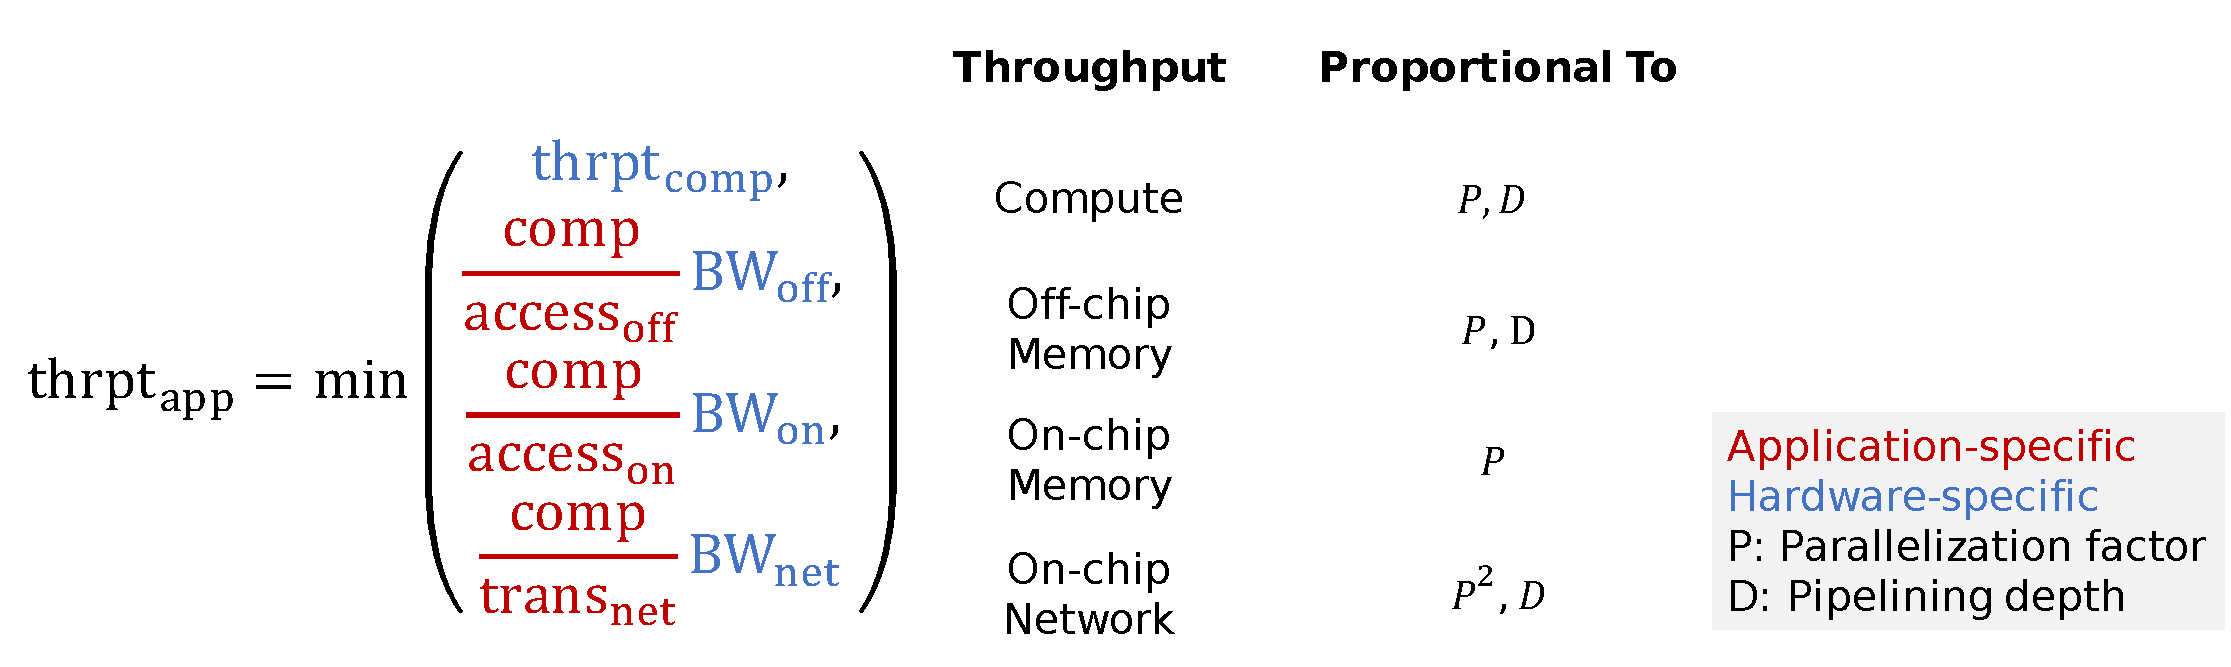
\includegraphics[width=1\textwidth]{figs/perfmodel.pdf}
\caption[High-level performance model of a spatial architecture]{
High-level performance model of a spatial architecture. 
}
\label{fig:perfmodel}
\end{figure*}

\Cref{fig:perfmodel} shows a high-level performance model of a spatially pipelined and parallelized
reconfigurable architecture.
Due to pipelined execution, the performance of a spatial architecture is dominant by throughput as
supposed to latency. 
Compute, on and off-chip memory accesses, and network become a integrated pipeline, 
where performance is limited by the pipeline stage with lowest throughput.
The red terms in the equation are application-specific and capture the compute, memory, or IO-bound characteristics.
The blue terms are the available bandwidth and FLOPS on the hardware.
While the compute and memory access in application increases linearly with parallelization factor and pipelining depth,
the required network bandwidth from application increases quadratically with increasing parallelism.
This means as we going to larger chip size, the network bandwidth must grow super linearly in
order to achieve a perfect performance scaling, unless exploring pipeline parallelism.

RDAs need the right amount of interconnect flexibility to achieve good resource utilization; 
an inflexible interconnect constrains the space of
valid application mappings and hinders resource utilization. 
Furthermore, 
in the quest to increase compute density, RDA data paths now 
contain increasingly coarse-grained processing blocks such as pipelined, vectorized functional 
units~\cite{plasticine, piperench, xilinx-acap}.
Plasticine, as an example, has a 512-bit vector bus, which necessitates coarser communication and higher on-chip interconnect bandwidth to avoid creating performance bottlenecks. 
Although many hardware accelerators with large, vectorized data paths have fixed local networks~\cite{brainwave}, there is a need for more
flexible global networks to adapt to future applications.
Consequently, interconnect design for these RDAs involves achieving a balance between the often conflicting requirements of high bandwidth and high flexibility.

\section{The Gap between High-Level DSLs and Dataflow Accelerators}

\begin{figure*}
\centering
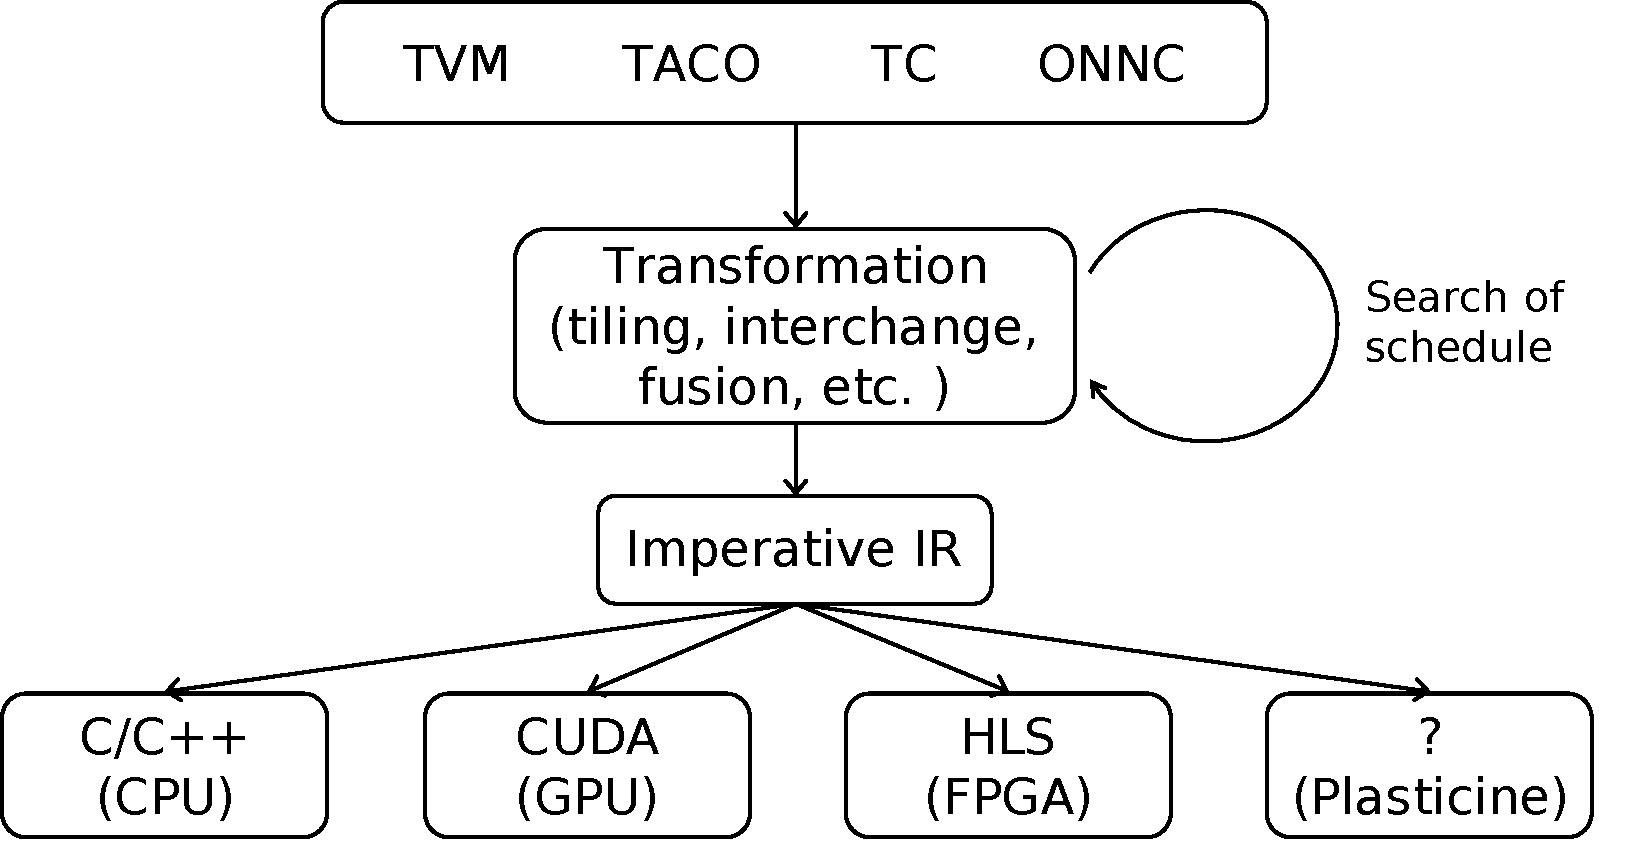
\includegraphics[width=0.6\textwidth]{figs/highlevel.pdf}
\caption[Big picture of accelerator compiler stack]{
  Big picture of accelerator compiler stack.
}
\label{fig:bigpic}
\end{figure*}

Recent years have seen a rise in interests in hardware accelerators, primarily motivated by AI applications. 
Research in software infrastructure for these accelerators, however, is just emerging.
Unlike CPUs, these accelerators do not support a standard ISAs, alleviating the overhead from
layers of abstractions and the burden of backward compatibility. 
Nonetheless, lack of a common abstraction makes it very hard to sharing compiler infrastructure
across accelerators. 

\section{Contribution}

In this work, we start by detailing the key considerations involved in building an RDA network, including those arising from network design, RDA architecture, and the characteristics of spatially mapped applications.
Network designs must be carefully considered because vectorization magnifies inefficiencies: the increased network area of a vectorized design ensures that any overhead has a significant impact.
Next, we evaluate the performance, area, and power requirements of several interconnection designs using cycle-accurate simulation and ASIC synthesis of a switch and router with a \SI{28}{nm} industrial technology library.
We then explore a variety of design points, including static, dynamic, and hybrid networks, decreased flit widths and VC counts for dynamic networks and different flow-control strategies for static networks.

We show that RDA network designs must consider application characteristics and the execution model of the underlying architecture.
Performance scales strongly with network bandwidth, with an 8x average performance gap between the best and worst configurations. 
The hybrid network gives the best network energy-efficiency: a 1.83x average improvement over the static network. On pipelined architectures,
hybrid networks can also match the performance per area of higher bandwidth, purely static networks with less than 8\% performance loss.

The key contributions of this paper are:
\begin{enumerate}
    \item An analysis of key communication patterns exhibited by spatial architectures.
    \item A network-aware compiler flow that efficiently targets static, dynamic, and hybrid networks with varying granularities.
    \item A quantitative analysis of the performance, area, and energy trade-offs involved in choosing an RDA network, using benchmarks drawn from various application domains.
\end{enumerate}

\section{Outline}

%\chapter{Background (WIP)}

\section{Execution Schedules of Reconfigurable Architectures} 
\begin{figure*}
\begin{subfigure}[b]{0.34\textwidth}
\inputminted{python}{code/spatialeg2.py}
\caption {
}
\end{subfigure}
\hfill
\begin{subfigure}[b]{0.65\textwidth}
\centering
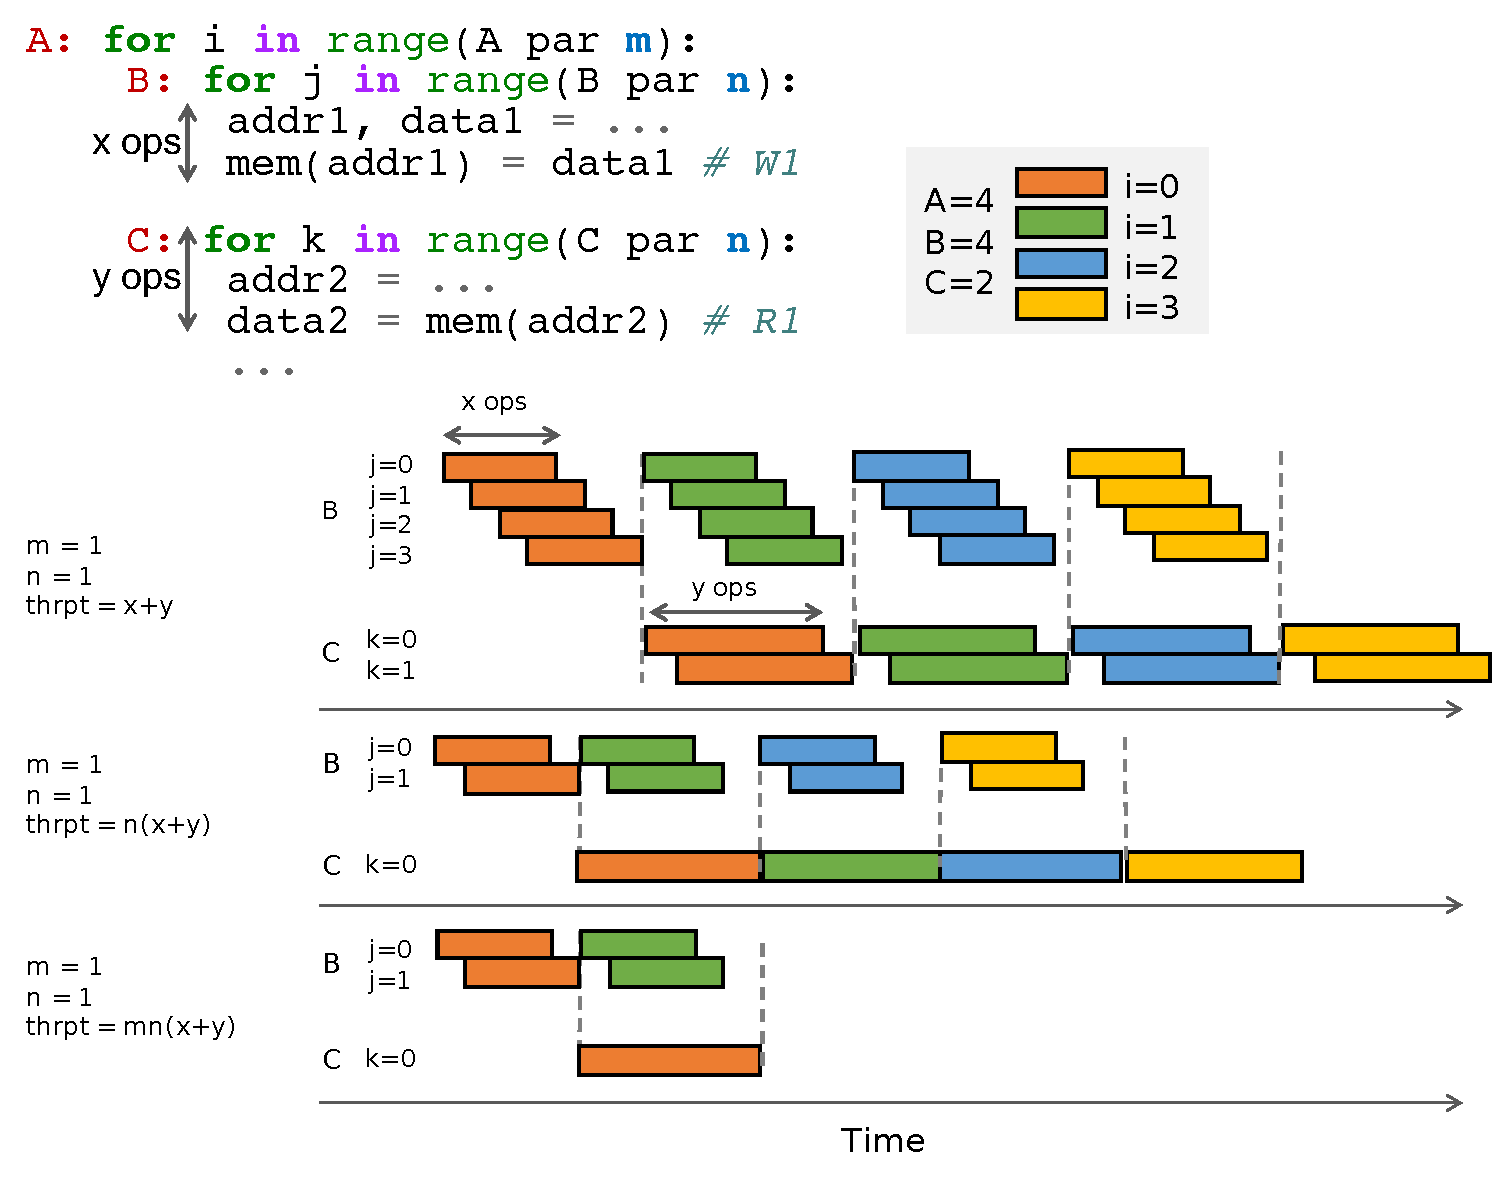
\includegraphics[width=1.0\textwidth]{figs/pipeexec.pdf}
\caption {
}
\end{subfigure}
\caption[Hiearchical pipelining and parallelization on spatial architecture]{
Hierarchical pipelining and parallelization in spatial architecture.
(a) illustrates the runtime and throughput of a hierarchically pipelined and parallelized program on
a reconfigurable spatial architecture. 
At inner level, instructions within each basic
block are fine-grained pipelined across iterations of the inner most loop. 
At outer level, the inner loops are coarse-grained pipelined across the outer loop iterations.
Exploiting multiple levels of pipeline parallelism gives a total throughput of $x+y$ operations per
  cycle, where \emph{x} and \emph{y} are number of operations in the basic blocks.
(b) Vectorizing the inner most loops B and C by \texttt{n} increases the throughput to $(x+y)n$.
(c) Parallelizing the outer loop A by \texttt{m} further increases the throughput to $(x+y)mn$.
}
\label{fig:pipeexec}
\end{figure*}

\begin{figure*}
\centering
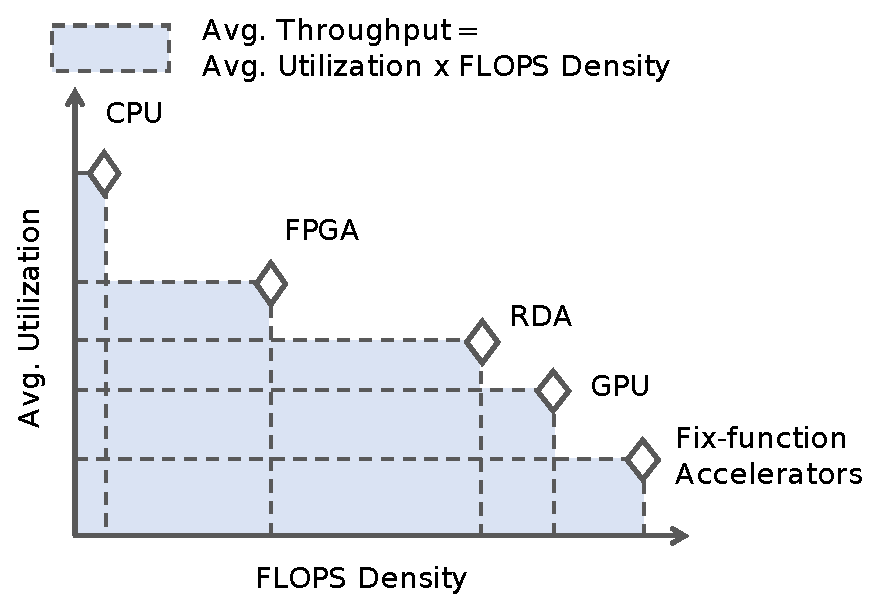
\includegraphics[width=0.4\textwidth]{figs/peakutil.pdf}
\caption[Average utilization vs. peak compute density tradeoff]{
 Average utilization vs. peak compute density tradeoff among different architectures.
}
\label{fig:peakutil}
\end{figure*}

\begin{figure*}
\centering
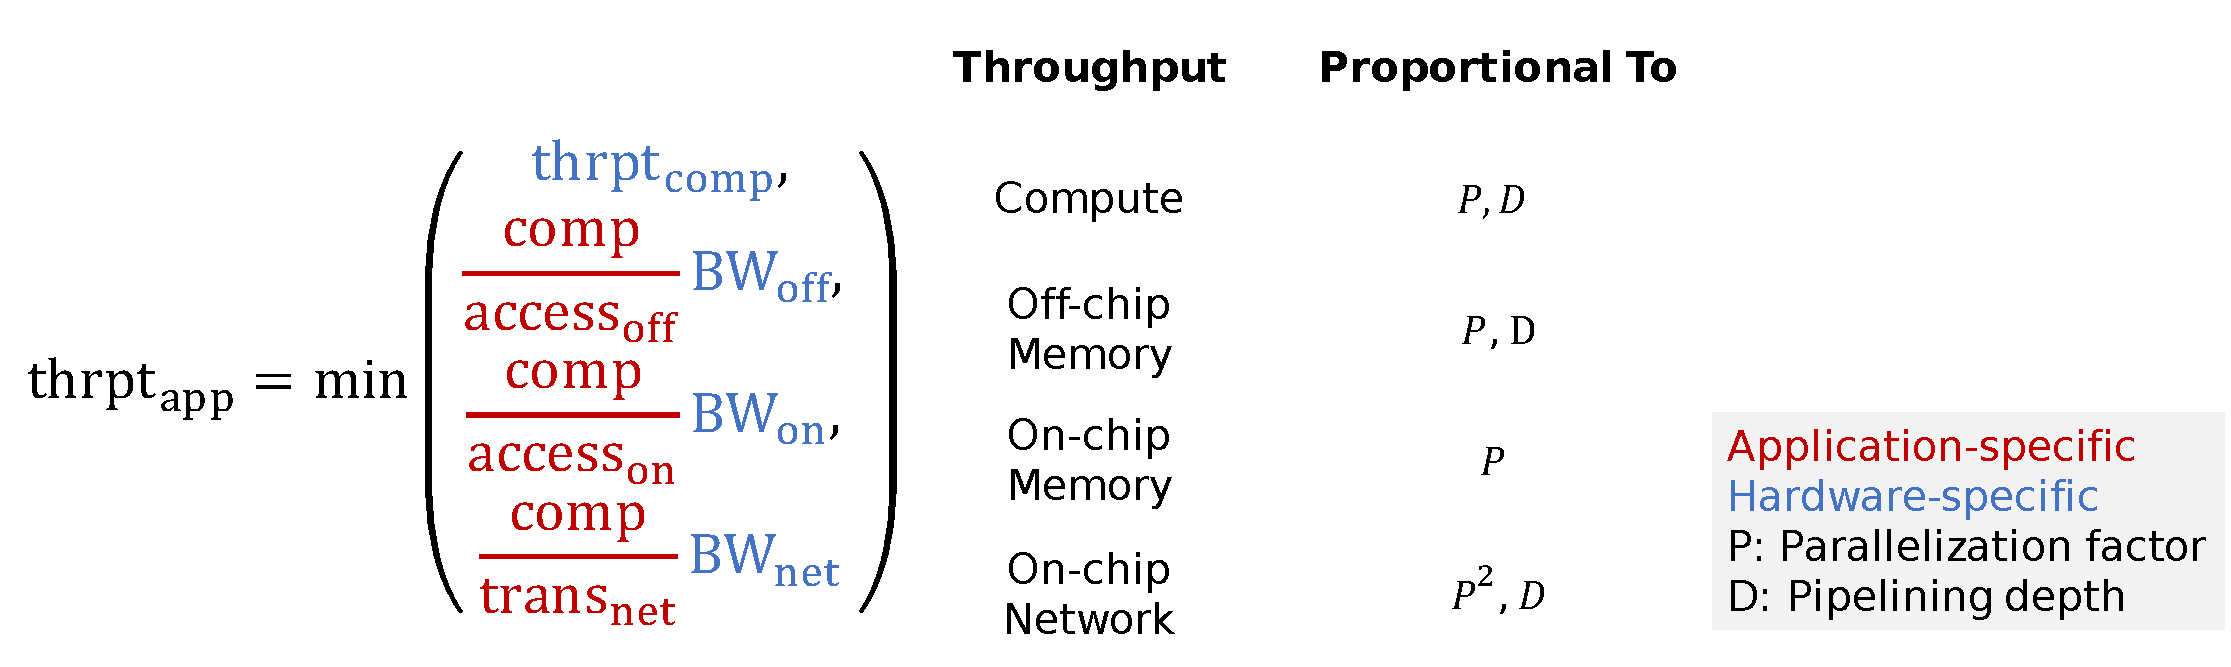
\includegraphics[width=1\textwidth]{figs/perfmodel.pdf}
\caption[High-level performance model of spatial architectures]{
High-level performance model of spatial architectures
}
\label{fig:perfmodel}
\end{figure*}

The key advantage of reconfigurable spatial accelerators, compared to processor-based architectures, 
is the ability to explore multiple levels of pipeline parallelism. 
In traditional Von Neumann architectures~\cite{vonneumann}, like CPUs and GPUs,
a computer consists of a processing unit that performs
computation, a memory unit that stores the program states, and a control unit that tracks execution
states and fetch the instruction to execute. This computing model inherently assumes that
instructions with in a program are executed in time, maximizing the flexibility to 
context switching between different workloads dynamically.

Reconfigurable accelerators are a direct violation of the von Neumann execution model; 
instructions are statically imbedded in the datapath and executed in space as supposed to in time.
One of the disadvantage of reconfigurable hardware is paying the resource cost for infrequently
executed instructions, making it unsuitable for control-heavy workloads that traditional
processors are efficient at.
On the other hand, RDAs are particularly competitive in providing high-throughput, 
low-latency, and energy-efficiency acceleration for data-analytical workloads.
Data-analytical workloads encompass a wide domains of applications, including image processing,
recognition, machine translation, digital signal processing, network processing, etc.
These applications exhibits a rich amount of data-level parallelism with relatively static control
flow.

\Cref{fig:pipeexec} shows an example of hierarchical parallelism and pipelining exploit by
a spatial architecture.
The overall compute throughput of a parallelized and pipelined program is 
the product of the total parallelization factors and pipelining depth.
By exploring multiple dimensions of concurrency in the program, spatial architecture is more likely
to achieve a good compute throughput for a wide range of applications.
For applications that are expensive to parallelize due to irregular access patterns, spatial
architectures can increase on the pipelining dimension;
for application with embarrassingly parallel workloads, spatial architecture can budget most
resource on increasing parallelism.

Another benefit of pipelined execution is easier to achieve good memory performance.
Data accessed by different stage of the pipelines are stored in discrete scratchpads 
instead of a shared cache; improving the effective on-chip bandwidth and capacity.
Using explicitly managed scratchpad also tends to improve locality and 
eliminate cache performance issues, such thrashing.
Across kernels, pipelined execution reduces the amount of off-chip accesses for intermediate
data.
SIMT architectures, like GPUs, relying on high-bandwidth DRAM technology, such has HBM, to sustain
the compute throughput of massively parallelized threads.
While providing over 10x more bandwidth than traditional DDR technologies, HBM is very limited in
capacity, around 16GB as supposed to on the orders of TB for DDR.
As a result, the limited off-chip capacity often restricts the type of applications that
GPUs can support.

%\begin{table*}
  %\centering
%\begin{tabular}{lccc}
  %\toprule
 %Concurrency Level & Instruction & Data & Task/Kernel  \\ \midrule
 %Parallelsim & CPU,\rda & CPU,GPU,\rda & CPU,\rda  \\
 %Pipelining & \rda & \rda & \rda \\
 %\bottomrule
%\end{tabular}
%\caption[Concurrency level explored by different architectures]{
  %Concurrency level explored by different architectures
%}
%\label{tab:conclevel}
%\end{table*}


%\section{Low-level Native Programming Interface of Plasticine}
Similar to FPGA high-level synthesis tools, \name provides a high-level imperative programming
abstraction and synthesizes the program to execute on a reconfigurable accelerator. Targeting an \rda, however,
is much more challenging than targeting FPAGs due to \rda's stringent mapping constraints. 
Unlike FPGAs, \rdas cannot map arbitrary RTL functionality. 

Taking Plasticine as an example, 
the hardware has collection of memory tiles (PMUs) and compute tiles (PCUs). 
The mesh global network can be statically configured to connect any tiles with guaranteed in-order 
transmission of packets over arbitrary network latency.

\subsubsection{Pattern Compute Unit (PCU)}
As the major compute work horse of the architecture, a PCU contains a 6-stage SIMD pipeline with 16 SIMD lanes. 
Unlike a processor core, the PCU can only statically configure six vector instructions throughout the
entire execution.
Additionally, the six instructions must be branch-free in order to be fully pipelined across stages.
At runtime, the SIMD pipeline executes the same set of instructions over different input data.
Software can configure the SIMD pipeline to depend on a set of input streams and
produce a set of output streams. 
There are three types of streams---single-bit control streams, 32-bit word scalar streams, and
16-word vector streams---corresponding to three types of global networks.
Execution of the PCU is triggered by the arrival of its input dependencies and back pressured by
the downstream buffers.
The PCU also contains configurable counters, which can be chained to produce the values of nested
loop iterators used in the datapath. 

\begin{figure}
  \begin{subfigure}[b]{0.5\textwidth}
    \inputminted{python}{code/contextfull.py}
    \caption{Declarative configuration}
    \label{fig:contexta}
  \end{subfigure}
  \hfill
  \begin{subfigure}[b]{0.4\textwidth}
    \inputminted{python}{code/context.py}
    \caption{Imperative configuration}
    \label{fig:contextb}
  \end{subfigure}
  \caption[Example PCU configuration]{
    Pseudo PCU configuration.
    (a) shows the simplified declarative-style configuration for the SIMD pipeline context in a PCU.
    Each PCU context can produce a set of output streams as a function of input streams and counter
    values.
    By configuring when each stream is enqueued and dequeued using signals from the chained counters, 
    these streams are effectively read and written within different loop bodies.
    (b) shows the equivalent configuration in a imperative-style on the right.
    On the left, the \texttt{valid} signal of the inner most counter \texttt{j} is high whenever the context is
    enabled. The context is implicitly triggered whenever its input streams \texttt{streamA},
    \texttt{streamB}, and \texttt{streamC} are non-empty and output stream \texttt{outputD} is ready.
    The declarative configuration also specifies a pipeline register (PR) to holds output of each stage
    and explicitly forward live variables across stages. 
    For simplicity, these details are omitted in the imperative-style on the right and
    \Cref{sec:regalloc} gives more details on register allocation for the SIMD pipeline.
  }
  \label{fig:context}
\end{figure}

We refer to the program graph that can be executed by the SIMD pipeline as a \term{compute context} or
simply \term{context}. 
A context includes the branch-free instructions mapped across SIMD stages, the input and output 
streams, and associated counter states and control configurations.
\Cref{fig:contexta} shows example of simplified pseudo assembly code to program a PCU context.
The control signals of the configurable counters, such as counter saturation or \term{counter done}
signals, can be used to dequeue and enqueue the input and output streams, respectively.
The counter bounds (i.e. min, max, and stride) can also be data-dependent using values from the 
scalar input streams. Compared to other data-flow architectures, the data-flow engine in Plasticine 
is more flexible in that it allows dynamic enqueue and dequeue window for its input and output streams.
\emph{This feature enable Plasticine to support complex control hierarchy, suchas  non-perfectly nested loops and
branch statements, across contexts even though individual contexts can only executes instructions that are
control-free}. 

\Cref{fig:contextb} represents the effective execution achieved in an imperative-style program.
For simplicity, we will use the imperative-style configuration in the later discussion.
However, it is important to notice that there is a one-to-one translation from the 
declarative-style configuration to the imperative-style, but not in the reverse way.
%There are many restrictions on structure of the program in the imperative-style. 
For example, the loops needs to be perfectly nested (only stream accesses can occur in the outer
loops).
\Cref{fig:contextrestrict} gives more details on operations supported by the PCU and programming
restrictions in the imperative programming style.

There is no global scheduler to orchestrate the execution order among contexts---the execution is purely
streaming and data-flow driven. 
The only way to order the execution of two contexts without a data-dependency is to 
introduce a control \term{token} between two contexts acting like a dummy data-dependency.
This restriction eliminates the need of long-travelling wires and communication hot spot caused by a
centralized scheduler, which  again improves the clock frequency and scalability of the architecture.

\subsubsection{Pattern Memory Unit (PMU)}
PMUs hold all distributed scratchpads available on-chip. 
Each PMU contains 16 SRAM banks with
32-word access granularity. The PMU also contains pipeline stages specialized for address
computation. Unlike SIMD pipelines in PCUs, these pipeline stages are non-vectorized and can only 
perform integer arithmetics. 
The address produced by the address pipeline is broadcasted to 16 banks with a configurable offset added to each bank.
In contrast to PCU SIMD pipeline that has to be programmed atomically, the address pipeline stages 
within PMUs can be sliced into a write and a read context, triggered independently.
In addition to compute stages, resources such as I/O ports, buffers, and counters are also shared across contexts.
It is the software's responsibility to make sure total resources consumed by all
contexts does not exceed resource limits of the PMU.
All contexts within PMU have access to the scratchpads with unprotected order. For instance, to
restrict a read context to access the scratchpad after the write context, the software must explicitly allocate
a token from the write context to the read context.
\name automatically generates required control tokens across context such that the memory access order is
consistent to the one from high-level program order.

Unlike most accelerators at this scale, Plasticine does not have any shared global on-chip memory. 
This design dramatically improve the memory density and scalability of the architecture 
by eliminating hardware complexity and overhead to support complex cache coherence protocol.
%% TODO: add a sentence commenting on the network bandwidth
On the other hand, however, the burden of maintaining consistent view of a logical memory mapped
across distributed scratchpads is left to the software.
The software must explicitly configure synchronizations across PCUs and PMUs, taking into account
that the network can introduce variable latency on both control and data path.
One of the major contribution of \name is to hide these synchronization burden from the programmer
and still provide a programming abstraction of logical memories with configurable bandwidth and 
arbitrary capacity that fits on-chip.

\subsubsection{DRAM Interface}
The Plasticine architecture provides access to four DDR channels on the two sides of the
tiled array, as shown in \Cref{fig:plasticine}. 
Each side has a column of DRAM address generator (DAG) specialized to generate off-chip
requests. Like compute pipeline in PMUs, the pipeline in DAG is also non-vectorized with integer
arithmetics. Each DAG can generates a load or a store request streams to the off-chip memory. All
streams can access the entire address space of the DRAM, with in-order response within each stream
and no ordering guaranteed across streams. To provide off-chip memory consistency, \name allocates
synchronizations across request generator and response receiver contexts to preserve memory ordering
specified in the program.

\section{Compiler Overview}

\begin{figure*}
\centering
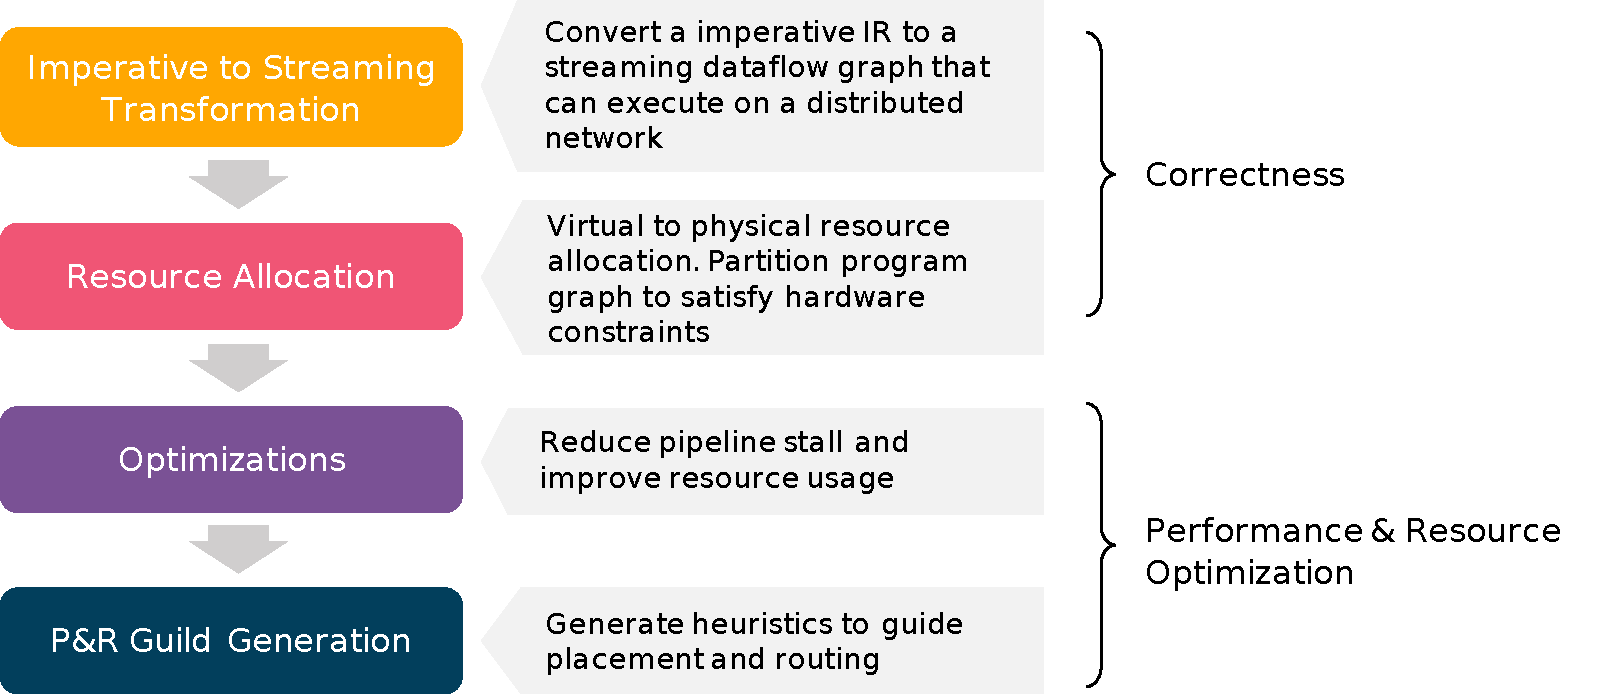
\includegraphics[width=1\textwidth]{figs/sarastack.pdf}
\caption[\name Compiler Flow]{\name Compiler Flow}
\label{fig:flow}
\end{figure*}
 
In this section, we describe a systematic approach to compile applications described in an
imperative front-end language with into a purely declarative and distributed dataflow graph that can
run on Plasticine.
\Cref{fig:flow} shows the compilation flow to perform this translation between the two paradigms.
At high-level, \name allocates distributed on-chip resources to execute the program in spatially parallelized and
pipelined fashion.
\name automatically generates synchronization across distributed units to provide strong 
memory consistency for a imperative program, on an architecture that does not guarantee memory
ordering across multiple access streams.
This synchronization is purely point-to-point introducing minimum performance overhead, which
maximizes scalability of the architecture.
\name further virtualizes resources allocation and hides the underlying resource constrains on
this hierarchical architecture from the programmers.

First, \name takes the input Spatial IR and performs the \term{virtual allocation}.
A virtual unit (VU) is our intermediate representation that captures computations that will be
mapped onto a physical unit (PB), such as a PCU and PMU.
Each VU can contain multiple contexts. However, a VU can be mapped to a PU only if the aggregated
resource usage of all contexts in the VU can fit in the PU. The PU can also limits the maximum 
number of contexts it can support, and has resources that cannot be split across contexts.
Additionally, messages across VUs are mapped across the global network, and must tolerate arbitrary 
amount of network latencies; messages within a single VB across contexts takes only a single cycle.
In the first phase, \name generates p2p synchronizations across contexts such that 
the execution is the same as if there are centrolized scheduler scheduling each level of the 
nested control hierarchy in the original program.
The allocation phase generates a virtual unit data-flow graph (VUDFG) with appropriate
synchronizations, such that the on-chip distributed execution produces the same result as if the program is
sequentially executed.

At the end of the allocation phase, a virtual unit can consume as much resource as the program
requires. The second phase is \term{physical allocation}, where \name assign each VU to a
PU that processes the required resources. If no PU can execute a VU, \name tries to partition the
VU into multiple VUs to eliminate constraint violation. If there is insufficient PU or the
VU cannot be partitioned, the mapping process fails with appropriate hint to the programmer for the
limiting resources.

Throughout the first two phases, \name introduces various \term{optimizations} that either reduce the
resource cost of the VUDFG, or alleviates potential performance bottleneck in streaming pipelined execution.
After all VU fits in at least one type of PU, \name performs a global optimization that merges 
small VUs into a larger VU to reduce resource fragmentations.

At the end the previous phase, each VB is tagged with a PB type that can fit the VB, and it is up to the
\term{placement and routing (PaR)} phase to determine where the VB will be finally placed.
\name can perform static analysis on the traffic pattern and generate heuristics for PaR to
reduce runtime congestion.

In the following sections, \Cref{sec:control} describes conversion from imperative paradigm with
nested control hierarchy to the distributed streaming data-flow execution.
\Cref{sec:decompose} details program-partitioning passes that decompose program over distributed resources.
\Cref{sec:opt} enumerates several optimizations in \name, and \Cref{sec:par} discuss about PaR and
heuristic generation.

\begin{figure*}
\centering
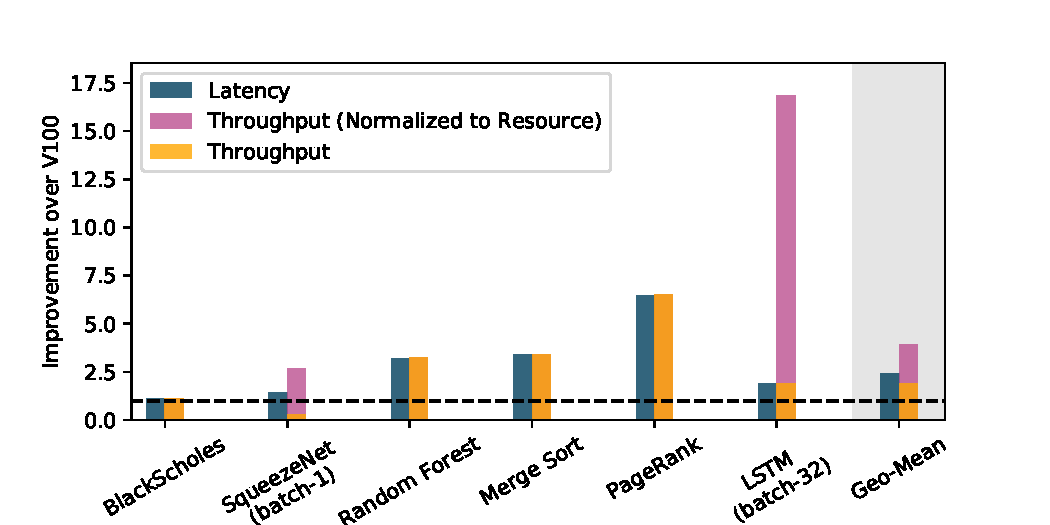
\includegraphics[width=1\textwidth]{figs/slide_gpu.pdf}
\caption[Performance comparison with V100 GPU]{
  Plasticine's latency and throughout improvement over V100 GPU.
  The evaluated Plasticine architecture has area footprint of 352$mm^2$ at 28nm.
  V100 GPU has area footprint of 815$mm^2$ at 12nm.
  Both platforms have the same off-chip bandwidth at 1TB/s with HBM technology.
  Yellow and blue bars show the raw measured speedup in throughput and latency, respectively.
  To account for the resource discrepancy, the pink bar shows the normalized throughput
  for compute-bound application--SqueezeNet and LSTM, which scales performance with additionally
  on-chip resources.
}
\label{fig:peakutil}
\end{figure*}

%\section{High-Level Compiler (WIP)} 

\begin{figure*}
\centering
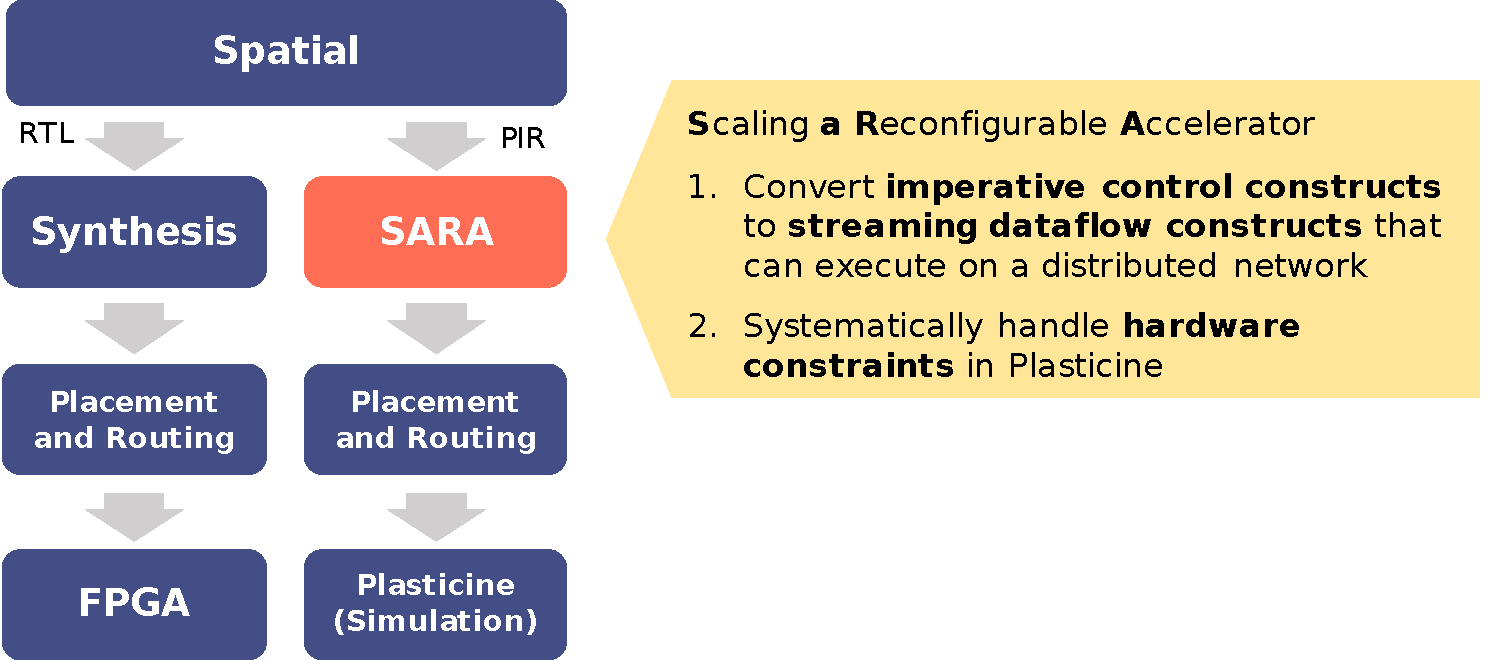
\includegraphics[width=1\textwidth]{figs/spatialstack.pdf}
\caption[Spatial Stack]{Spatial Stack}
\label{fig:spatialstack}
\end{figure*}

Although \name takes Spatial as front-end, the compilation techniques in \name can be equally
applied to other imperative langauges with nested loop constructs, such as C-based high-level
syntehsis language, the backend of Halide IR, and other DSLs at the similar abstraction level. 
Using Spatial as our front-end language has the advantage that the language is designed for
reconfigurable hardware, such that it can express valid execution schedule that can be exploit by
spatial architectures natively in the language.

%% Memory model
The data structure reprsented most exisitng imperative languages IR often marries to the
CPU's virtual memory model. LLVM-based compilers, for example, treats data collections as pointers to a shared
global address space, without distinguising what data are stored on-chip vs. off-chip.
This is CPU provides the memory abstraction that any data within the global address space 
can be equally accessed and the hardware implicitly manage the data movement between on and off-chip 
access by brining
Accelerators on the other hand, has explicitly managed on-chip scratchpads, that is not a cached
version of main memory data implicitly managed by the hardware.
The idea is to have the algorithm, which has better understanding of the data characteristics, to
explicitly control what data gets moved on and off-chip to maximize locality.
Other important static analysis in synthesis compilers, such as banking analysis, requires the
compiler to have the global view all access patterns on a data structure.
Therefore, modeling the data structures as disjoint memory space is much more suitable 
than pointers to a shared memory for reconfigurable architectures.

Spatial currently does not capture procedure calls in the IR; all functions are inlined and does not
share resources. A future work is to use synchronization mechanism in \name to implement true procedure
call on a spatial architecture.

Without lost of generality, we use python-style pseudo code to represents the front-end programming
abstraction the the rest of our discussion.

Most compilers for CPU uses a control flow graph to represent the control of a imperative program.
The control flow graph implicitly assumes the program is executed in time, which make it unsuitable
for analysis of a reconfigurable architecture that executes the program in space. 
Spatial uses a control hierarchy in the IR to captures the scheduling of the program.
The control hiearchy uses a tree structure to represent the nested control constructs, making it
easier to search the LCA of two controllers.
\Cref{fig:spatialegpar} shows an example of a control flow graph vs. a control hiearchy.
The controller at each level of the hierarchy corresponds to a control primitive, such as a loop, or
a branch statement. 
A basic block is attached to each \emph{inner most} controller including instructions
and memory accesses to user declared data-structures.
If the program has instructions in a outer loop, Spatial automatically inserts a \emph{unit}
controller to wrap the floating instructions.
\name takes the backend of Spatial IR as the input, which is an control hierarchy after loop
unrolling.

\begin{figure*}
\centering
\begin{subfigure}[b]{0.4\textwidth}
\inputminted{python}{code/spatialegpar.py}
\caption{Pseudo Spatial example}
\end{subfigure}
\hfill
\begin{subfigure}[b]{0.58\textwidth}
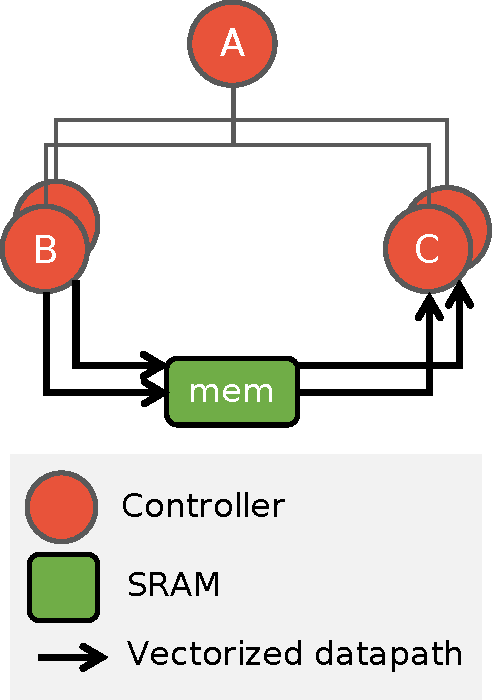
\includegraphics[width=1\textwidth]{figs/spatialir.pdf}
%\missingfigure[figwidth=1\textwidth]{Spatial IR}
\caption{Schematic Spatial IR}
\end{subfigure}
\caption[Spatial Example]{
  Pseudo example of \name's front-end language.
  (a) shows the an example of \name's front-end language. The actual front-end Spatial is a
  Scala-embeded DSL. For simplicity and generality, we use a python style pseudo code to show an
  language with similar abstraction. The `par` keyword indicates outer loop unrolling factor, and
  the `vec` keyword is followed by a inner-loop vectorization factor.
  When an iterator is vectorized, instructions using the vectorized iterator is automatically
  vectorized as well. When unrolling the outer loop \texttt{A}, the enclosed loop body and
  next-level control hierarchy are duplicated, as suggested in (b).
  Each loop in (a) corresponds to a controller in (b). The inner most controllers \texttt{B} and
  \texttt{C} each contain a basic block within instructions within the inner most loops.
}
\label{fig:spatialegpar}
\end{figure*}



%\chapter{Compiler} \label{sec:compiler}

In this section, we introduce the compiler framework---\name---that targets Plasticine
architecture from high-level programs described in the Spatial language. 

In the following sections, \Cref{sec:control} describes conversion from an imperative paradigm with
a nested control hierarchy to the distributed streaming dataflow execution.
\Cref{sec:resalloc} details program-partitioning passes that decompose program over distributed resources.
\Cref{sec:opt} enumerates several optimizations in \name, and \Cref{sec:par} discuss about PaR and
heuristic generation.

\section{\name Compiler Overview} \label{sec:compileroverview}

In this section, we introduce the compiler framework---\name---that targets Plasticine
architecture from high-level programs described in the Spatial language. 
There are two challenges to map Spatial applications to Plasticine. 

First, unlike a FPGA, Plasticine cannot map arbitrary RTL functionality.
In the Spatial abstraction, the execution order of the program is organized by a control hierarchy, where
each level of the controller schedules the execution of the next level controllers.
When mapping the example in \Cref{fig:spatialegpar} onto a FPGA, the outer controller \emph{A}
sends an enable signal to each child controller, signaling back the parent controller when
completed. If the user choose to sequentially execute the outer loop \emph{A}, the parent
controller enables the child controllers one at a time; if the user choose to metapipeline
(coase-grain pipeline) the outer loop \emph{A}, the outer controllers enables multiple child
controllers in a pipelined fashion.

\begin{figure*}
\centering
  \centering
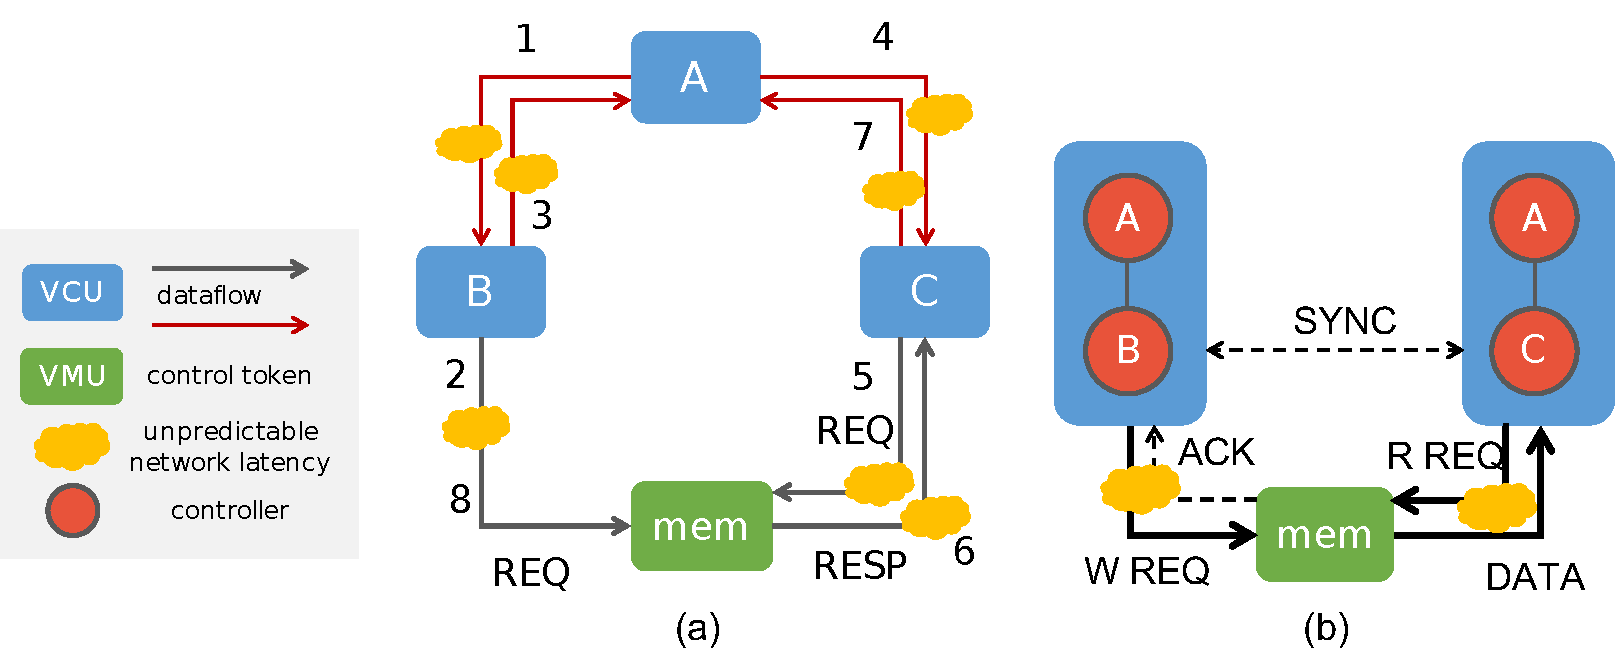
\includegraphics[width=0.8\textwidth]{figs/centralctrl.pdf}
\caption{
  (a) A na\"ive mapping strategy to map the control hierarchy onto Plasticine.
  All units are distributed across an on-chip network that can introduce unpredictable latency.
  The number on the edges indicate the order of event.
  Here we show a scenario where read requests from \emph{C} do not observe the write requests from
  \emph{B} that appears earlier in the program order due to network latency between \emph{B} and
  \emph{mem}.
  (b) Distributed controllers in \name. Each innermost controller makes a copy of all enclosing
  controllers. The signals from these controller are used to generate synchronization between
  distributed compute unit. To address the problem in (a), the memory also needs to provide an write
  acknowledgment per write request for synchronization.
}
\label{fig:centralctrl}
\end{figure*}

To achieve the same execution schedule on Plasticine in a na\"ive approach, 
we can map each controller in the hierarchy into a PU
, sending control signals to schedule the next level 
controllers distributed in other PUs, as shown in \Cref{fig:centralctrl} (a).
This strategy suffers from the expensive network round-trip delays between the parent and child controllers.
To be scalable at a high clock frequency, Plasticine networks are pipelined at each switch,
introducing multiple cycles of network delay across PUs on the control path.
Therefore, the multi-cycle handshaking signal between the parent and the child can introduce significant pipeline bubbles
that undermines performance.
Additionally, this scheme creates a communication hotspot around the parent controller \emph{A} as
loop \emph{A} gets unrolled, which is devastating for a coarse-grained reconfigurable architecture
like Plasticine that has much less routing resource than a FPGA.
Furthermore, synchronizing the compute only is insufficient to ensure memory effects are observed by
the remotely distributed accessors, as shown in \Cref{fig:centralctrl} (a).

To address this challenge, we want to eliminate any of the centralized schedulers for the outer
controllers.
At high-level, \name achieves this by performing loop division for each outer controller, such that
all innermost controllers are perfectly nested, as shown in \Cref{fig:centralctrl} (b).
\name then allocates synchronization tokens across distributed innermost controllers.
All innermost controllers have their own copies of the outer controllers, which are used
to control when to send and consume the control tokens.
These control token ensures the execution order of the inner controllers is the same as if they are
scheduled by a centralized outer controller. Instead of synchronizing all inner controllers under an
outer controllers, \name only synchronizes the ones accessing the same memory, such as \emph{B} and
\emph{C} in \Cref{fig:spatialegpar}. This limits the synchronization among a small set of distributed nodes, 
making our design much more scalable.

The second challenge in this mapping process is that controllers in the spatial hierarchy
can consume arbitrary amount of compute and memory resources, exceeding the capacity of individual
PUs. For instance, a user might write a memory multiple times throughput the program with writers 
mapped to different PUs. The physical scratchpad, however, only has a single write
port. \name needs to virtualize resources, composing or time sharing them when software usage
exceeding the hardware limit.

\begin{figure*}
\centering
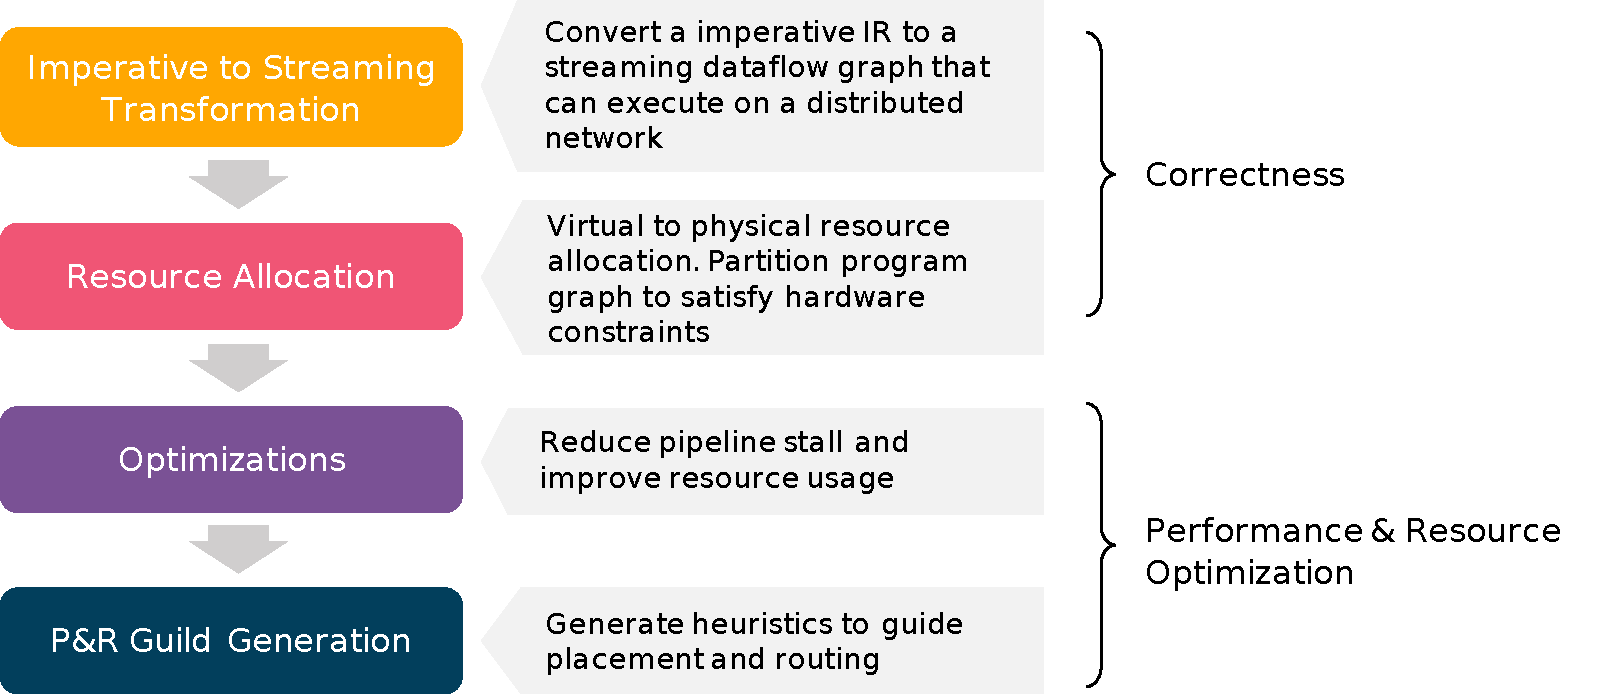
\includegraphics[width=1\textwidth]{figs/sarastack.pdf}
\caption[\name Compiler Flow]{\name Compiler Flow}
\label{fig:flow}
\end{figure*}
 
In the following sections, we describe a systematic approach to compile applications described in an
imperative front-end language to a purely declarative and distributed dataflow graph that can
run on Plasticine. \Cref{fig:flow} shows \name's compilation flow.

\Cref{sec:control} expands on the \term{imperative to streaming transformation} that
addresses the first challenge.
\name allocates distributed on-chip resources to execute the program in spatially parallelized and
pipelined fashion with approperate synchronizations.
A virtual unit (VU) is our intermediate representation that captures computations 
%that will be
%mapped onto 
within the boundary of
a physical unit (PU), such as a PCU and PMU.
Each VU can contain multiple contexts, if their aggregated resources usage can fit in a PU.
The hardware can limit the maximum number of contexts a PU can support and has resources that cannot be split across contexts.
Most importantly, \name needs to ensure messages across VUs, which are mapped across the global network, must tolerate an arbitrary amount of network latencies; messages within a single VU across contexts takes only a single cycle.
The transformation phase generates a virtual unit dataflow graph (VUDFG) with appropriate
synchronizations, such that a streaming pipelined execution over distributed on-chip resources produces the same result as a
parallelized program executed in time.
At the end of the allocation phase, a virtual unit can consume as much resources as the program
requires. 

\name further virtualizes resource allocation and hides the underlying resource constrains on
this hierarchical architecture from the programmers.
\Cref{sec:resalloc} dives into the \term{resource allocation} phase, where \name assign each VU to a
PU that processes the required resources. If no PU can execute a VU, \name partitions the
VU into multiple VUs to eliminate constraint violations. If there is insufficient PU or the VU cannot be partitioned, the mapping process fails with appropriate hints to the programmer for the
limiting resources.

Throughout the first two phases, \name introduces various \term{optimizations} that either reduce the
resource cost of the VUDFG, or alleviates potential performance bottleneck in the streaming
pipeline.
After all VU fits in at least one type of PU, \name performs a global optimization that merges small VUs into a larger VU to reduce resource fragmentations.
\Cref{sec:opt} enumerates the optimizations \name perform.

The output of the resource allocation phase is a VUDFG with a tagged PU type for each VU.
It is up to the
\term{placement and routing (PaR)} phase to determine where the VU will be finally placed.
Right before PaR, \name performs static analysis on the traffic pattern and generate heuristic guild
for the placer to reduce routing congestion.
\Cref{sec:par} details the PaR algorithm and heuristic-guild generated by \name.


\section{Distributed Control Flow}
\label{sec:control}

The input to \name is the backend of the Spatial IR, which is an control hierarchy after loop
unrolling.
The controller at each level of the hierarchy corresponds to a control primitive, such as a loop, or
a branch statement. A basic block is attached to each \emph{inner most} controller including instructions
and memory accesses to user declared data-structures.
\Cref{fig:spatialir} shows an example of a program and a schematic Spatial output IR.

\begin{figure*}
\centering
\begin{subfigure}[b]{0.4\textwidth}
\inputminted{python}{code/spatialeg.py}
\caption{Pseudo Spatial Example}
\end{subfigure}
\hfill
\begin{subfigure}[b]{0.58\textwidth}
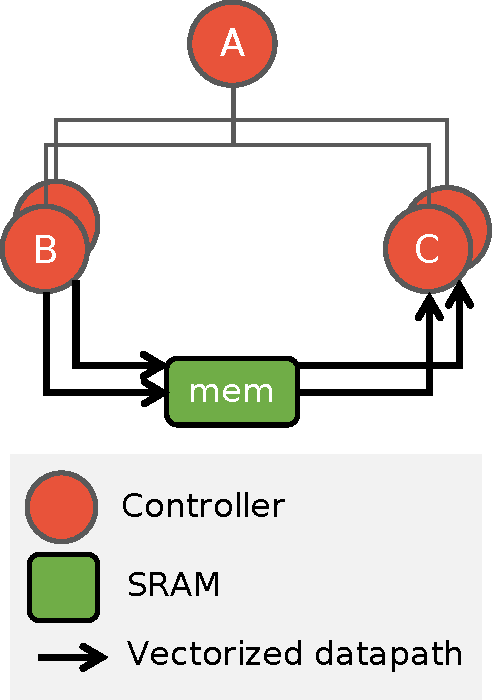
\includegraphics[width=1\textwidth]{figs/spatialir.pdf}
%\missingfigure[figwidth=1\textwidth]{Spatial IR}
\caption{Schematic Spatial IR}
\label{fig:spatialir}
\end{subfigure}
\caption[Spatial Example]{Pseudo example of \name's front-end language}
\end{figure*}

\begin{figure*}
\centering
%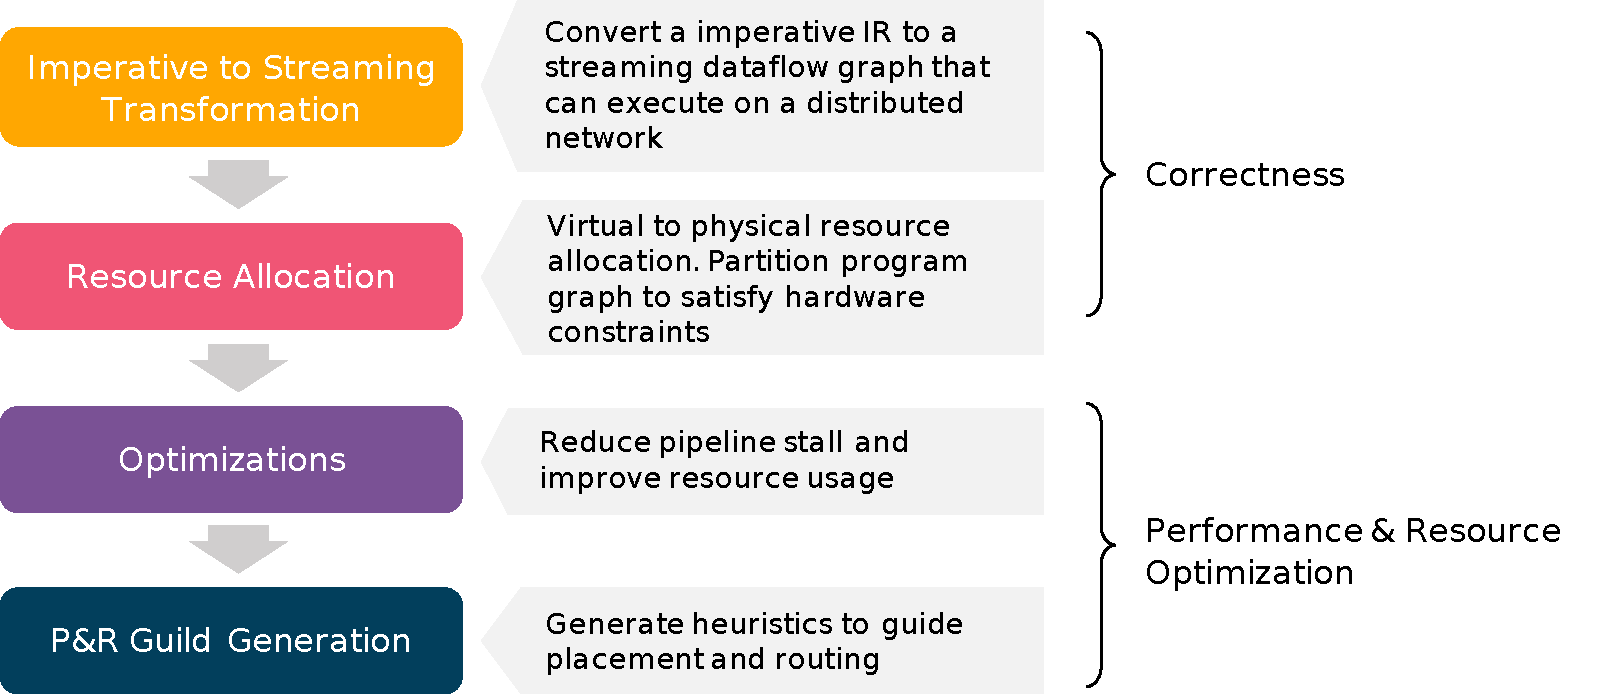
\includegraphics[width=1\textwidth]{figs/sarastack.pdf}
\missingfigure[figwidth=1\textwidth]{Controller duplication}
\caption[Context allocation]{Context allocation}
\label{fig:contextalloc}
\end{figure*}

%\begin{figure*}
%\centering
%\caption[Spatial IR]{Spatial IR}
%\label{fig:spatialir}
%\end{figure*}

As a start, \name allocates one virtual memory to hold each on-chip data structure, and 
one context to execute each basic block within the inner most controllers. 
A basic block maps naturally to a context, as instructions within a basic block are control-free. 
Next, \name makes a copy of all controllers enclosing the basic block in the corresponding context, as
shown in \Cref{fig:contextalloc};
these controllers are later converted to counters and control configurations supported by the
hardware. 
With these controllers, contexts can repeat execution for expected number iterations. However,
data-structures written and read by different contexts are accessed in random order.
The insight is that \emph{as long as all contexts accessing a shared memory with expected program order,
the final result is identical to a sequentially executed program}.
Unlike traditional out-of-order execution, where hardware and compiler look for independent instructions to
execute concurrently, \name starts with all basic blocks executing in concurrent contexts.
\name then introduces synchronizations to maintain consistent access order as expected by the 
program \emph{only} among contexts accessing a shared memory. 
This way, \name introduces minimum p2p synchronizations among small groups of contexts; contexts
accessing different memories are naturally parallelized without impacting the final output.
\todo{walk through an example here}.

To order the execution order or two contexts, \name allocates a single-bit \term{control token} as 
an access grant to the shared memory and passes it between contexts. 
This control token is no different from a regular data-dependency.
By controlling {\em where}, {\em how}, and {\em when} to pass the token, \name 
is able to maintain a consistent update ordering between the pipelined and parallelized actors that access the shared memory.

%In a na\"ive approach, we can map each controller in the hierarchy into a VB (\Cref{fig:centralctrl}).
%This strategy suffers from expensive network round-trip delays between the parent and child controllers.
%If the parent controller is an unrolled loop, the parent needs to synchronize with all child controllers, which creates an undesired communication hot spot.
%\Cref{fig:centralctrl}(a) shows an example where synchronization {\em just} between parent and child controllers can produce an incorrect result due to unpredictable network latency.

%The alternative approach explores a different way to execute the expected control schedule correctly. 
%The minimum required synchronization to produce the correct result is to ensure that the computations access the intermediate results in a consistent matter as if the control schedule is strictly enforced. 
%This can be achieved via p2p synchronizations \emph{only} between computations that access a particular shared memory.
%The execution order of computations that access different memories does not need to be enforced, as they do not impact the program outcome.
%Therefore, as long as the compututation is executed with the expected number of iterations and the memories are updated consistently, there is no need for any extra synchronization.
%Next, we walk through how \name{} achieves this in more concrete detail.


\subsection{Synchronization} 
\label{sec:sync}
We refer to an access to the memory in the input graph as a \emph{declared access}, as supposed to accesses executed at runtime.
For example, multiple accesses across loop iterations are counted as a single declared access.

\paragraph{Where.}
\name only allocate resource to synchronize actors if their declared accesses can potentially interfere.
Whether two declared accesses interfere depends on the type of accesses, the type of the memory, and location of the accesses in the control hierarchy.
For every declared access, \name{} checks other accesses of the same memory appeared earlier in the program order for a possible forward dependency, and later in the program order for a possible loop-carried dependency (LCD). 
Two declared accesses A and B have no dependency if their least-common ancestor (LCA) controller executes only one of the children at anytime (from a branch), or all children in parallel (from an unrolled loop).
The LCD exists between B to A, if B occurs later in the program order, and A and B are surrounded by a loop.
To detect LCD, \name checks if a loop exists among two accesses' LCA controller and LCA's ancestor controllers.
For a dual-ported SRAM, all other accesses need to be synchronized to: share address ports for read-after-read (RAR) and write-after-write (WAW); 
enforce true data-dependency for read-after-write (RAW); and
prevent the overriding of read data for write-after-read (WAR).
\gist{If the memory is multi-buffered (by the user or high-level compiler), we do not need to synchronize for WAR~\cite{dhdl} (the writer writes to a different buffer than the reader does). }
The DRAM interface permits concurrent read streams and, hence, RAR does not need to be synchronized.

\begin{figure*}
\centering
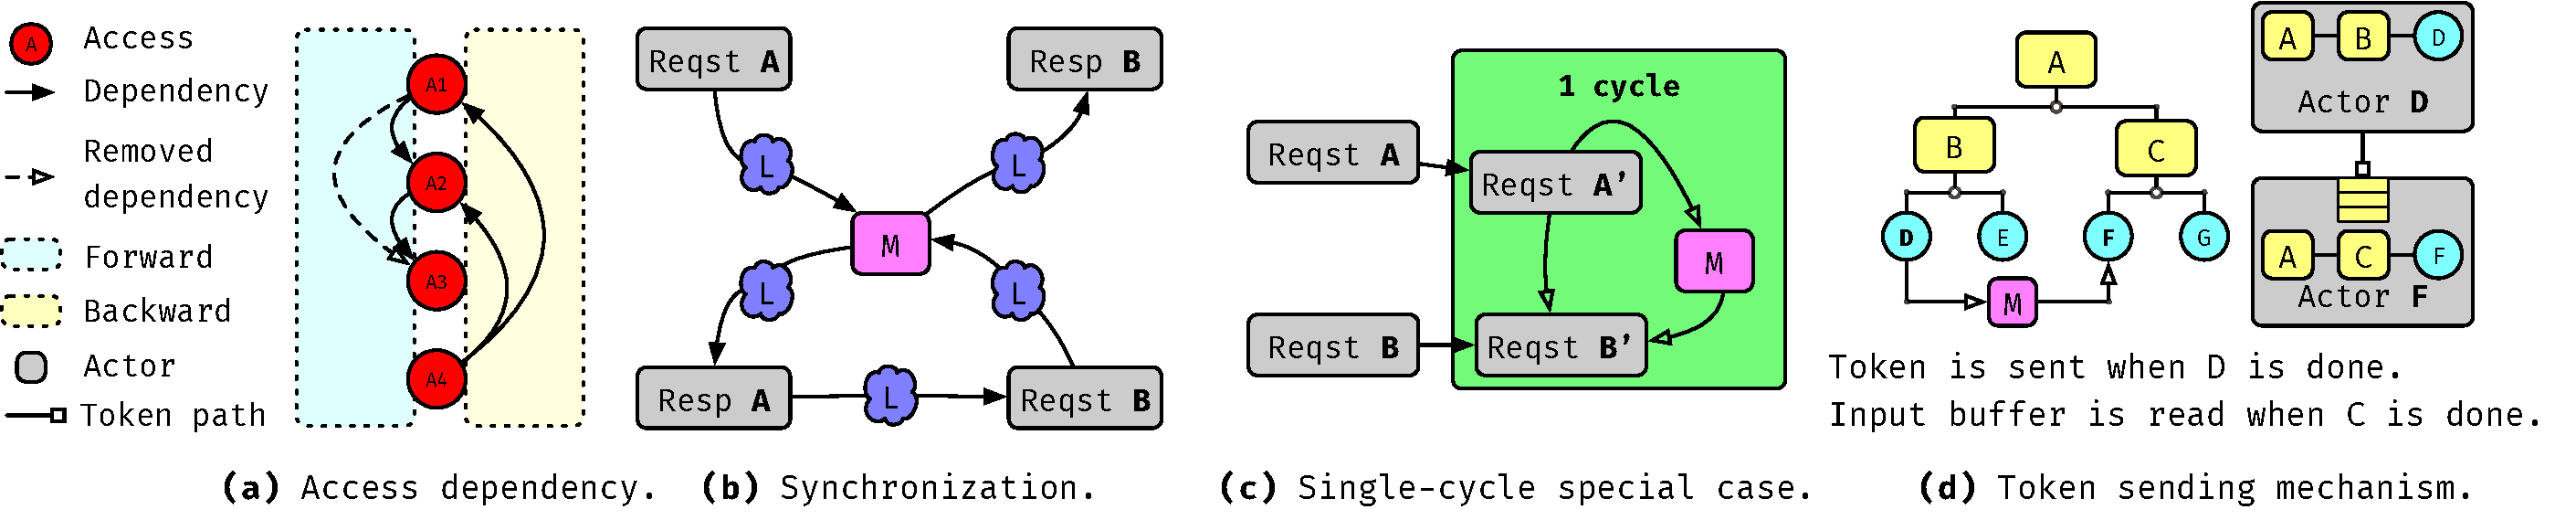
\includegraphics[width=1.0\textwidth]{figs/synch_mech.pdf}
\caption{
    (a) Access dependency graph.
    (b) Synchronization of two accesses on the same memory.
    (c) Single-cycle special case.
    (d) Actors uses local states of controller hierarchy to determine when to send a token.
}\label{fig:depgraph}\label{fig:token}\label{fig:tokentrick}\label{fig:tokenwhen}
\end{figure*}
%\ms{repeated caption, rather give a single caption.}

\paragraph{How.} For each intermediate memory, \name{} builds a dependency graph for all its declared accesses (\Cref{fig:depgraph}(a)).
Enforcing all dependencies in this graph may not be necessary as dependencies between $A_1$ and $A_2$, and $A_2$ and $A_3$ already capture the dependency between $A_1$ and $A_3$.
Therefore, \name{} performs a transitive reduction (TR) on the graph to keep the minimum number of dependency edges that preserve the same ordering \cite{tr}.
Since TR on a cyclic graph is NP-hard, we perform TRs on the forward and backward LCD graphs, separately.
Notice, dependencies between accesses touching different buffers of a multi-buffered memory is less rigid than accesses touching the same buffer.
Therefore, we can only remove an edge if all dependencies on the equivalent path have a stronger or equivalent dependency strength than the strength of the removed edge.

To eliminate the round-trip overhead between the memory and the computation, 
\name{} duplicates the local states and expressions required to generate the requests in a separate actor as the one that handles the responses.
For write accesses, the memory provides an acknowledgment for each request received, used by \name for synchronization.
The request actor generates requests asynchronously as soon as its data-dependencies are cleared, pushing all requests to memory until back-pressured.
To order a declared access A before a declared access B
\name creates a dummy dependency between the actor that accumulates the response of access A ($resp_A$) and the actor that generates requests for access B ($reqst_B$) (\Cref{fig:token}(b)).
To enforce LCD from access B to access A, \name introduces a token from $resp_B$ to $reqst_A$, and initializes the token buffer (input buffer receiving the token) with one element to enable the execution of the first iteration.
If the LCD is on a multi-buffered memory, the LCD token is initialized with the buffer depth number of elements to enable A for multiple iterations before blocked by access B.

These are general schemes we use on any types of memory (including DRAM and on-chip memories) with unpredictable access latency.

\subparagraph{Special Case: Single-Cycle Access}
For a memory with guaranteed {\em single-cycle} access latency, such as registers and statically banked SRAMs that are guaranteed conflict-free, we can simplify the necessary synchronization (\Cref{fig:tokentrick}(c)).
Instead of synchronizing between $resp_A$ and $reqst_B$, we allocate two stateless actors $reqst_A'$ and $reqst_B'$ within {\emph the same} VB as the accessed memory that forwards requests from $reqst_A$ and $reqst_B$, respectively.
Next, we forward the token going from $reqst_A$ to $reqst_B$ to go through $reqst_A'$ to $reqst_B'$ instead, and configure the token buffer in $reqst_B'$ with the depth of one for serialized schedule and depth of M for multi-buffered schedule. 
We no longer need to insert the LCD token, as the stiff back pressure from the token buffer in $reqst_B'$ will enforce the expected behavior.
This optimization only works if the sender and receiver of the token buffer are physically in a single VB where the memory is located.
In this way, when $reqst_B'$ observes $reqst_A'$s token, $reqst_B'$ is guaranteed to observe the memory update from $reqst_A'$ because the memory also has single-cycle access latency.

\subparagraph{Memory Localization}
We perform another specialization on non-indexable memories (registers or FIFOs), whose all accesses have no explicit read enables.
Instead of treating them as shared memories, \name{} duplicates and maps them to local input buffers in all receivers, no longer requiring tokens.
The sender actor pushes to the network when the token is supposed to be sent, and the receiver dequeues one element from the input buffer when the token is supposed to be consumed.
This dramatically reduces the synchronization complexity of non-indexable memory in the common case.

\paragraph{When.}
\name{} configures the actors to generate the token using their local states at runtime.
For FIFOs, the token is generated and consumed every cycle when the producer and receiver actors are active.
For register, SRAM, and DRAM the program order expects that the producer and consumer writes and inspects the memory once per iteration of their LCA controller, respectively.
Since the producer and receiver both have their outer controllers duplicated in their local state, they have independent views for one iteration of the LCA controller, which is when the controller in their ancestors (that is the immediate child of the LCA controller) is completed (\Cref{fig:tokenwhen}(d)).
The {\em done} signals of these controllers are used to produce and consume the token in actors, independently.

\subsection{Data-Dependent Control Flow}
Using the synchronization discussed in \Cref{sec:sync}, we can support control constructs that typically are not supported on most RDAs, such as branch and a while convergence loop.
The controllers in the input graph can also have data dependencies, such as loop ranges. 
The dynamic-loop ranges are handled as data dependencies to actors with \emph{memory localization} described in \Cref{sec:sync}.
The branch condition is also treated as a data-dependent enable signal of controllers under branch clauses.
If the controller is disabled, it is considered {\em done} immediately.
Output tokens depending on the {\em done} signal will be immediately sent out.
For a memory written inside a branch statement and read outside the branch (with a branch miss), the writer actor immediately sends out the token to the receiver
as soon as the branch condition is resolved. 
With a branch hit, the controller waits until its inner controller completes before raising the {\em done} signal.
%This way, the 
A similar scheme is used to implement the while loop, where the while condition is a data-dependency of stop signal of controller X. 
The producer of the while condition also consumes its own output as an LCD. 
The condition is then broadcast to all other actors under the same while loop. 
The {\em done} signal of the while loop is raised when the condition's data-dependency evaluates to true.
At this point, actors accessing memory within the while loop will send the token to access actors outside of the while loop, and enable them to access the intermediate memory.

After all actors and shared resources are allocated and synchronized, we simply put each actor and shared resource into their own VBs.
The actors with single-cycle special case (\Cref{sec:sync}) must be put in the same VB as the shared memory.


\section{Resource Allocation} \label{sec:resalloc}

The output of the imperative to dataflow transformation discussed in \Cref{sec:control} is a VUDFG that 
can execute on a Plasticine with physical units (PUs) that have infinite resources.
The \emph{Resource Allocation} phase enforces and addresses constraint violations given 
the specification of the Plasticine units. 
At the end of this phase, \name assigns each VU in the VUDFG graph to a PU type with required
resources; the placer then takes the type assignments and determines the final placement.

Accelerators often have heterogeneity in compute resources to improve efficiency for common
special operations.
In Plasticine, PMUs and AGs have specialized compute pipelines for address calculation that are 
less capable than the compute pipeline in PCUs.
However, heterogeneity tends to reduce average utilization because different applications, and even the same application with different data sizes, can vary highly in the desired ratio among different
resource~\cite{tz_rnn}.
A compute-bound application, for example, can heavily underutilize the AGs and PMUs.
To address this problem, \name models the virtual to physical assignment as a constraint satisfaction problem; 
each VU consumes a set of resources and can only be assigned to a PU if the PU processes the required resources. 
%Instead of using heuristics to assign certain a type of VU to a type of PU, we
\Cref{tab:resource} shows the types of resources \name models in Plasticine's heterogeneous units.
For example, special connection to off-chip memory interface is
also treated as a type of resource in the AG, which forces virtual contexts accessing DRAM to map to AGs. 
On the other side, regular contexts with non-vectorized fixed-point operations can also be mapped to
spare AGs, which improves utilization.
\begin{table*}
  \centering
\begin{tabular}{lccccc}
  \toprule
  Feature & PCU & PMU & AG & Host Unit & Aggregation Function\\ \midrule
  Vector lane width & 16 & 16 & 1 & 1 & \multirow{2}{*}{MAX}\\
  \# pipeline register (PR) & 8 & 8 & 4 & 0 & \\ \hline
  \# stages & 6 & 10 & 5 & 0 & \multirow{6}{*}{SUM}\\
  Scratchpad banks & 0 & 16 & 0 & 0 &  \\
  Scratchpad capacity & 0 & 256kB & 0 & 0 & \\
  MergeBuffer & 1 & 0 & 0 & 0 & \\
  Splitter & 1 & 0 & 0 & 0 & \\
  Scanner & 1 & 0 & 0 & 0 & \\ \hline
  Operation types & fix $\cup$ float & fix & fix & $\varnothing$ & $\cup$ \\ \hline
  Reduction tree & \cmark & \xmark & \xmark & \xmark & \multirow{3}{*}{OR}\\
  Access to DRAM Interface & \xmark & \xmark & \cmark & \xmark & \\
  Access to Host IO & \xmark & \xmark & \xmark & \cmark & \\ \hline
  \# Vector Input & 6 & 6 & 4 & 0 & \multirow{6}{*}{G}\\
  \# Scalar Inputs & 6 & 6 & 4 & 16 & \\
  \# Control Inputs & 16 & 16 & 4 & 16& \\
  \# Vector Outputs & 6 & 6 & 4 & 0 & \\
  \# Scalar Outputs & 6 & 6 & 4 & 16 & \\
  \# Control Outputs & 8 & 8 & 2 & 16 & \\
 \bottomrule
\end{tabular}
\caption[Resources specification of heterogeneous units and aggregation function]{
  A list of resources \name models in four types of configurable units in Plasticine. The host unit
  models the host registers I/Os.
  MergeBuffer, Splitter, and Scanner are new hardware units introduced in \cite{gorgon} and recent work
  to support database and sparsity in Plasticine.
  The aggregation function indicates how to compute the aggregated resource cost when two contexts are merged
  into a single virtual unit (VU). G indicates the aggreated value is the output of a graph traversal of the
  merged graph. How to count \# I/O is discussed later in \Cref{sec:compsplit}.
  While the aggreation function of \#PR of two merged contexts is MAX, the \#PR of a
  context is the maximum number of live variables of its dataflow graph, which is also an output of
  a topological traversal.
  This table reflects a different Plasticine configuration as the original Plasticine in \cite{plasticine}.
}
\label{tab:resource}
\end{table*}

\begin{algorithm}
  \Fn(\tcc*[h]{Allocation Algorithm}){alloc(V, P, pruners)}{
    \KwData{V: a set of VUs from the VUDFG}
    \KwData{P: a set of all PUs on the hardware}
    \KwData{pruners: a list of constraint pruners to check
    and fixes constraint violations}
    \tcc{Initialize a complete bipartite graph}
    G = \KwNew BipartiteGraph()\;
    G[V] = P\;
    \tcc{Constraint resolution}
    prune(G, pruners)\;
    \tcc{Global merging}
    merge(G)\;
    \tcc{Heuristic check on whether assigning all VUs in V is feasible}
    check(G)\;
    \tcc{Virtual to physical assignment}
    backtracking\_assign(G)\;
  }
  \vspace{0.5cm}
  \Fn(\tcc*[h]{A recursive pruning function}){prune(G, pruners)}{
    \KwData{G: bipartite graph between VUs and PUs}
    \KwData{pruners: a list of constraint pruners to check
    and fixes constraint violations}
    \KwResult{The function update G by removing VU-PU edges that violates constraints guarded by
    pruners. The function may fail and raise an exception.}
    \tcc{All PUs on the hardware}
    P = G.values()\;
    \For{pruner \KwTo pruners}{
      \For{v \KwTo G.keys()}{
        \For{p \KwTo G[v]} {
          \If{pruner.cost(v) > pruner.cost(p)} {
            G[v] -= p\;
          }
        }
        \If{G[v].empty()} {
          \tcc{Partition VU v based on resource constraints registered in pruner. 
          Not all resources can be partitioned and this step may fail.
          If succeeded, the function returns a new set of VUs.}
          V' = pruner.partition(v)\;
          G' = \KwNew BipartiteGraph()\;
          G'[V'] = P\;
          prune(G',pruners)\;
          G -= v\;
          G[V'] = G'[V']\;
        }
      }
    }
  }
  \caption{Resource allocation. The bipartite graph \texttt{G} contains a bi-directional many-to-many
  map. \texttt{G[key]} returns the set of values connecting to the key (dom(key)), and \texttt{G[value]}
  returns the set of keys connecting to the value.
  \texttt{G[key] = value} connects an edge between key and value.
  \texttt{G[KeySet] = ValueSet} creates all-to-all connection between \texttt{KeySet} and
  \texttt{ValueSet}.}
  \label{algo:resalloc}
\end{algorithm}

\begin{algorithm}
  \Fn(\tcc*[h]{Assignment feasibility check}){check(G)}{
    \KwData{G: bipartite graph}
    \KwResult{Whether it is possible to assign all VUs in V with a different PU in P}
    \tcc{For every value set in \texttt{G}}
    \For{V \KwTo G.values().toSet()} {
      K = $\varnothing$\;
      \For{v \KwTo V} {
        \For{k \KwTo G[v]} {
          \If{G[k] $\subset$ V} {
            K += k\;
          }
        }
      }
      \If{|K| > |V|} {
        \KwRet{failure()}\;
      }
    }
    \KwRet{success()}\;
  }
  \caption{Heuristic check on whether it is possible to assign all key with an value in a bipartite
  graph. Given there are only a few types of hardware tiles, $G.values().toSet()$ is
  relatively small. This algorithm roughly runs in $O(|G.keys()|\times|G.values()|)$, which is
  still much faster than the backtracking assignment with exponential runtime.}
  \label{algo:check}
\end{algorithm}
 
%% backtracking_assignment(vu, dom)
As shown in \Cref{algo:resalloc}, the \emph{resource allocation} phase contains three steps:
\emph{constraint resolution}, \emph{global merging}, and \emph{virtual to physical assignment}.
\name uses a VU-PU bipartite graph (\emph{G}) to keep track of potential valid assignments between the two.
Initially, \emph{G} is initialized to a complete bipartite graph, i.e., all VUs can be assigned to
all PUs.
We refer to all PUs connected to a VU \emph{v} as the domain of \emph{v} in G, i.e. \emph{dom(v)}.

\paragraph{Constraint Resolution}
A list of constraint pruners, each considering a set of on-chip resources, 
incrementally remove the VU-PU edges that violate the resource constraints.
If a VU \emph{v} has an empty domain after pruning, the pruner attempts to fix the violation by
decomposing the VU into multiple VUs. 
Not all resources are composable, and the partitioning transformation may fail.
If succeeded, the partitioner generates a new set of VUs \emph{V'}. \name starts a new complete bipartite
graph between \emph{V'} and all resources \emph{P}, and recursively prune on \emph{V'}.
If succeeded, the original graph \emph{G} is updated with \emph{V'} and their pruned resources.

\paragraph{Global Merging}
After all VUs have at least one PU in the bipartite graph, \name triggers a global optimization that merges 
small VUs into a larger VU to reduce fragmentation in allocation.
Each type of resource has an aggregation rule to compute how the resource cost changes if two VUs are merged
together, as shown in \Cref{tab:resource}. 
Most aggregation rules are simple, such as addition, logical or, max, or union.
The in- and out-degree costs are tricker and will be detailed in \Cref{sec:compsplit}.

\paragraph{Virtual to Physical Assignment}
Next, \name performs a quick heuristic check on the bipartite graph to see if there exists a
possible assignment for all VUs with sufficient PUs (\Cref{algo:check}), and provide feedback on the limiting resources, otherwise.
Finally, \name assigns each VU to a PU type with a backtracking search on the pruned bipartite
graph.

This approach can be easily extended to handle new heterogeneous tiles in the architecture by registering
the tile with existing or new types of resources with aggregation and partitioning rules.
The rest of this section goes over two types of partitioning transformations--compute
partitioning in \Cref{sec:compsplit} and memory partitioning in \Cref{sec:memsplit}.
%We have another partitioner encoding valid rule to decompose a BlackBox IP block available on the RDA.

\subsection{Compute Partitioning} 
\label{sec:compsplit}

The {\em compute-partitioning} phase addresses VUs using more compute resources than any PU can provide. 
If a VU contains multiple contexts, \name{} first moves the contexts into separate VUs.
If a single context exceeds the resource limit, \name breaks down the dataflow graph in the context into multiple contexts and puts them in separate VUs.
During partitioning, \name maps each subgraph of the large dataflow graph into a new context, mirrors the control states of the original context, and streams live variables in between.
We can formulate the problem of how to partition in the dataflow graph as an optimization problem, shown in
\Cref{tab:partprob}.
The partitioner ``fixes'' the VU \emph{v} based on a single PU specification, albeit there are many potential PUs 
the decomposed VU can be mapped to.
Currently, we use a heuristic to select a PU type from \emph{dom(v)} right before the compute pruning 
as a guiding constraint for partitioning.

\begin{table*}
  \centering
\begin{tabular}{lp{12cm}}
  \toprule
  \textbf{Problem} & Partition the dataflow graph into subgraphs such that all subgraphs satisfy the constraints of a
  hardware unit. \\[0.9cm]
  \textbf{Objective }& Minimize the number of partitions and connectivity across partitions. \\[0.5cm]
  \textbf{Constraints} & 
  \begin{minipage}{12cm}
  \begin{outline}
  \0 Each partition must not exceeds the limit on the number of \vspace{-0.2cm}
    \1 live in/out variables (I/O ports) \vspace{-0.2cm}
    \1 operations (pipeline stages), \vspace{-0.2cm}
    \1 and live variables across operations (pipeline registers), etc.\vspace{-0.2cm}
  \0 No \emph{new} cycles can form across partitions other than the cycles in the original
  dataflow graph.
  \end{outline}
  \end{minipage}
  \\
 \bottomrule
\end{tabular}
\caption[Formulation of the compute partitioning problem]{
Formulation of the compute partitioning problem
}
\label{tab:partprob}
\end{table*}

Because the global network is specialized to handle efficient broadcasts, 
the in/out-degree of a partition counts the number of unique live-in/out variables, as supposed to
the number of edges across partitions.
In addition, the partitioned subgraphs cannot form {\em new} cycles; contexts waits for all
input dependencies and therefore cycles across contexts cause deadlock. 
Nonetheless, the original graph might contain cycles representing loop-carried dependencies, such as
accumulation. For these cycles, \name initializes the back edge of the cycle with dummy data to
enable execution.
\Cref{fig:parteg} shows examples of valid and invalid partitioning solutions.
\Cref{fig:partcycleeg} shows another partitioning example of a dataflow graph with cycles.

\begin{figure}
  \centering
  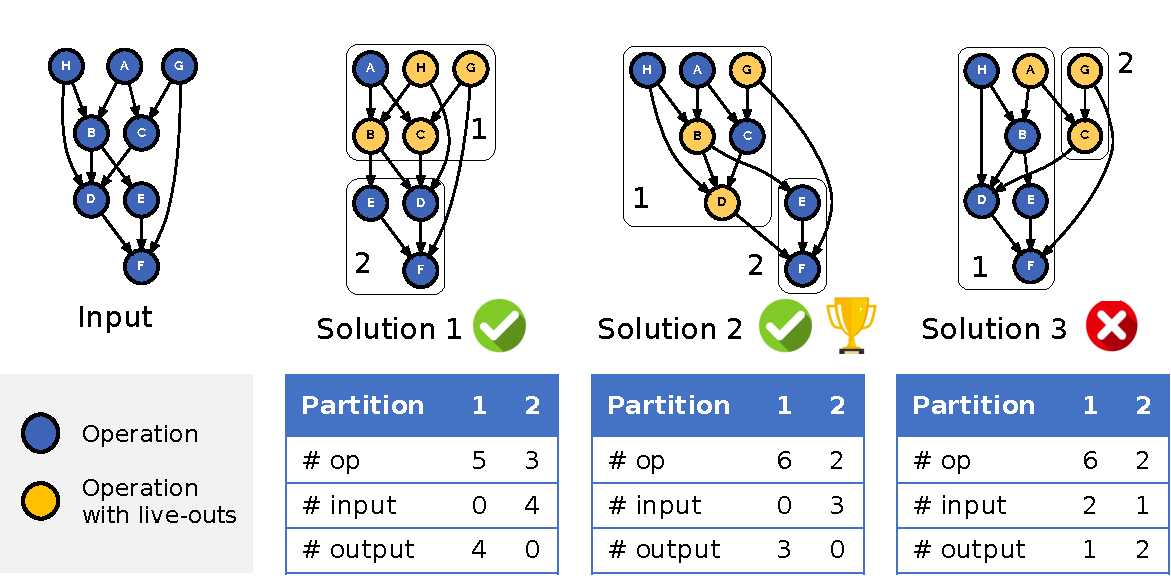
\includegraphics[width=1\columnwidth]{figs/parteg.pdf}
  \caption[Compute partitioning examples]{
    Compute partitioning examples. Solution 1 and 2 are both valid. Solution 2 is
    better because it has less number of broadcast edges across partitions (3 as supposed to 4 in Solution 1). 
    Solution 3 is an illegal partitioning due to the cycle between partition 1 and 2.
  }
  \label{fig:parteg}

  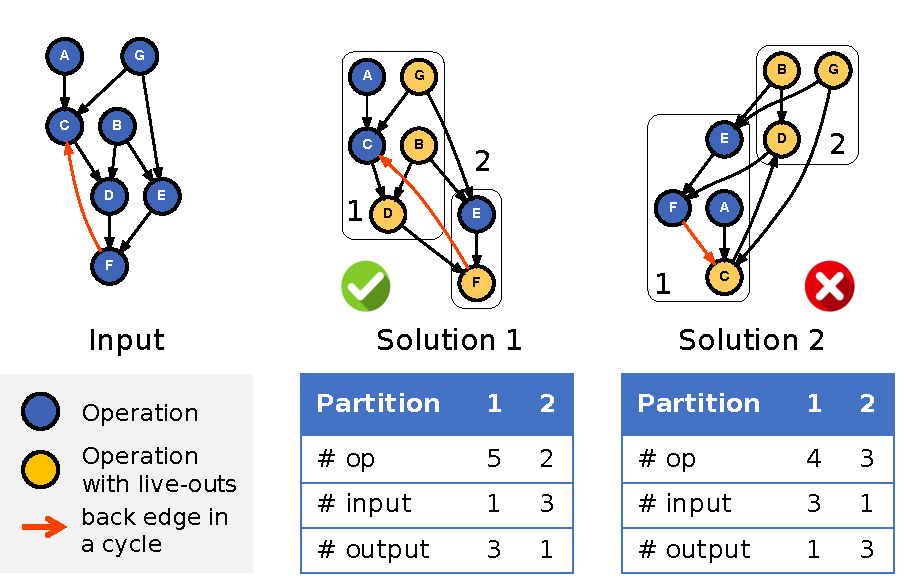
\includegraphics[width=0.8\columnwidth]{figs/partcycleeg.pdf}
  \caption[Compute partitioning examples with cycle]{
    Compute partitioning examples with cycle in the dataflow graph.
    Solution 1 is valid because there is no 
    cycle between partitions after removing the back edge in
    the original graph.
    Solution 2 is invalid because there is still cycle between partition 1 and 2 after
    removing the back edge.
  }
  \label{fig:partcycleeg}
\end{figure}

\paragraph{Community Detection}
The formulation of compute partitioning is similar to the community detection
problem\cite{community} that has a similar objective. 
The major difference is that the latter often takes the number of output partitions as an
input to the algorithm, whereas our problem partitions until all subgraphs satisfy all constraints.
Moreover, community detection algorithms do not enforce the cycle constraints. 
Finally, the edge connectivity in community detection counts the number of edges across partitions, 
as supposed to broadcast edges as in our problem.

\paragraph{Retiming}
Imbalanced data paths across partitions can cause pipeline stalls at runtime if the long-live path is not
sufficiently buffered.
To ensure full-throughput pipelining, \name needs to insert retiming buffers along the imbalanced data path across
partitions.
Retiming introduces new VUs in addition to the partitioned VUs, which attributes to the cost in
\Cref{tab:partprob}'s objective.

In the following sections, we present two algorithms to resolve the problem described in
\Cref{tab:partprob}:
a fast traversal-based algorithm providing a decent solution, and a slow convex
optimization-based algorithm providing an optimal solution.

\subsubsection{Traversal-based Solution}
To address the cycle constraint, the traversal-based algorithm performs a topological sort of the dataflow graph.
The topological sort ignores the back edges of the cycles during traversal. 
Starting from one end of the sorted list, the algorithm iteratively adds nodes into a partition
until it fits no more nodes. The algorithm then repeats the process with a new partition.
This approach guarantees that no cycle is introduced with $O(V+E)$ complexity, 
where $V$ and $E$ are the numbers of vertices and edges in the dataflow graph.

The partitioning result is a function of the traversal order.
We experienced with depth-first search (DFS) and breadth-first search (BFS) with forward and
backward dataflow traversal orders.
For DFS, we re-sort the remaining list each time starting with a new partition.

\subsubsection{Solver-based Solution}
The convex optimization solution models the problem as a node-to-partition assignment problem.
\Cref{tab:solver-eqns} gives our formulation and \Cref{tab:solver-variables} explains the notations
used in \Cref{tab:solver-eqns}.

\begin{table*}
  \centering
	\begin{tabular}{c | c | c | c}
		\textbf{Name} & \textbf{Type} & \textbf{Description} & \textbf{Definition / Default}\\\hline
		$\mathcal{N}$ & Constant & Enumeration of nodes to partition, numbered $\{n_i\}_i$ & - \\
		N & Constant, $\nnint$ & Number of operations to partition & $N = |\mathcal{N}|$\\
		P & Constant, $\nnint$ & Number of partitions to consider & $N$, or from heuristic \\
		$\mathcal{E}$ & Constant, $\{n_i \to n_j\}$& Directed edges representing dependence & - \\
		B & Variable, $\{0, 1\}^{N \times P}$ & Boolean Partitioning Matrix& - \\
		%p & Variable, $\nnint^N$ & Vector of mappings from node to assigned partition& $p = B \begin{bmatrix} 0 & 1 & \cdots & P-1\end{bmatrix}^T$\\
		$\projb{\cdot}$ & $\nnint \to \mathbb{B}$ & Function to convert a positive integer into a boolean& Supplemental Materials\\
		$\andf(\cdot, \cdot)$ & $\{0, 1\} \times \{0, 1\} \to \{0, 1\}$ & Boolean and of binary variables & Supplemental Materials \\ 
		$d_p$ & Variable, $\nnint^P$ & Vector of partition delays & - \\
		$d_n$ & Variable, $\nnint^N$ & Vector of node delays & - \\
		$\dest(n)$ & $\mathcal{N} \to \mathcal{P}(\mathcal{N})$& The set of nodes which depend on $n$& $\{n' | n' \in \mathcal{N}\ s.t.\ (n \to n') \in \mathcal{E}\}$\\
		$c_o$ & Constant, $\nnint$ & Maximum output arity of a partition & HW Spec \\
		$c_i$ & Constant, $\nnint$ & Maximum input arity of a partition & HW Spec \\
		$b_d$ & Constant, $\nnint$ & Maximum input buffer depth & HW Spec \\
		$K$ & Constant, $\mathbb{R}_+$ & Very Large Constant, used for constraint activation & $P \times N$ \\
		$\alpha_d$ & Hyperparameter, $\mathbb{R}_+$ & Retime merging probability multiplier& $\frac{1}{\max\{c_o, c_i\}}$ \\
	\end{tabular}
	\caption{Names and definitions used in the solver-based partitioning.}
	\label{tab:solver-variables}
\end{table*}

\begin{table*}
  \centering
  \newcommand\cola{1.6cm}
  \newcommand\colb{3.8cm}
  \newcommand\colc{9cm}
  \newcommand{\gcell}[2]{\Gape[#1cm][0cm]{\makecell[l]{#2}}}
  \begin{tabularx}{\textwidth}{cp{\colb}X}
    \toprule
		\textbf{Type} & \textbf{Description} & \textbf{Expression}\\\midrule
    \multirow{3}{*}{\makecell[l]{Cost\\Function}} & Allocated Partitions & $\Sigma_i \projb{\Sigma_j B_{i, j}}$\\

    & \makecell[l]{Additional Retiming\\Partitions}
    & $\alpha_d \Sigma_{n_i \to n_j \in \mathcal{E}} \projb{\max\{d_n(j) - d_n(i) - b_d, 0\}}$\\[0.3cm]
		\hline

    \multirow{12}{\cola}{\makecell[l]{\\\\Constraint}} & Partition Assignment & $ \forall n_i \in \mathcal{N}:\ \Sigma_j B_{i, j} = 1$\\[0.1cm]

    &\makecell[l]{Dependency\\Constraint} & $\forall n_i \to n_j \in \mathcal{E}:\ d_n(i) + 1[p_i \ne p_j] \le d_n(j)$\\[0.1cm]

    &\makecell[l]{Output Arity\\ Constraint} 
    &\makecell[l]{
      $\forall p \in [0, P):$ \\
      $\Sigma_{n_s \in \mathcal{N}} \andf(B_{s, p}, \projb{\max\{(\Sigma_{n_d \in \dest(n_s)} B_{d, p}) -$ \\
      $K \times B_{s, p}, 0\}}) \le c_o$
    }\\[0.7cm]

    &\makecell[l]{Input Arity Constraint\\ (vectorized)} & $\Sigma_{n_i \in \mathcal{N}} \max\{\projb{\Sigma_{n_j \in \dest(n_i)} B_{j, :}} - B_{i, :}, 0\} \le c_i \times \vec{1}$\\

		&Delay Consistency& 
    \makecell[l]{
    $\forall n_i \in \mathcal{N}:\ d_n(i) \le \min_j (d_p(j) + K - B_{i, j} \times K)$ \\
		$\forall n_i \in \mathcal{N}:\ d_n(i) \ge \max_j (d_p(j) + B_{i, j} \times K - K)$
    }\\[0.5cm]

		&Constant Validity& 
    \makecell[l]{
      $\forall n_i \in \mathcal{N}:\ d_n(i) \le K$\\
		  $\forall i \in [0, P):\ d_p(i) \le K$
    } \\
    \bottomrule
	\end{tabularx}
  \caption{Solver formulation for partitioning*.}
	\label{tab:solver-eqns}
\end{table*}

\begin{table*}
	\begin{tabular}{c | c | c | c}
		\textbf{Name} & \textbf{Type} & \textbf{Description} & \textbf{Definition / Default}\\\hline
		$\mathcal{C}_r$& $[\mathcal{N} \to \mathbb{R}_+,\mathbb{R}_+, [\mathbb{R}_+] \to \mathbb{R}_+]$ & List of per-node values, limits, and reduction& Supplemental Materials\\&& functions for reducible constraints& \\
		F & $\{0, 1\}^{N \times P}$ & Feasibility matrix, whether a partition can support a node& HW Spec \\ 
	\end{tabular}
	\caption{\Cref{tab:solver-variables} extension for solver-based merging, which is a generalization of the partitioning problem.}
	\label{tab:merging-variables}

	\begin{tabular}{c | c | c}
		\textbf{Type} & \textbf{Description} & \textbf{Expression}\\\hline
		Constraint & Feasibility Constraint & $ \forall i, j \in [0, N) \times [0, P):\ B_{i, j} \le F_{i, j}$\\
		& Reducible Constraints & $\forall j \in [0, P).\ \forall (c(\cdot), c_v, r(\cdot)) \in \mathcal{C}:\ r([c(n_i) \times B_{i, j}]_{n_i \in \mathcal{N}}) \le c_v$\\
	\end{tabular}
  \caption{\Cref{tab:solver-eqns} extension for solver-based merging*. The Retiming Partition objective is not used for merging.}
	\label{tab:merge-eqns}
  \scriptsize
  \raggedright
  \vspace{-0.3cm}
  *Expressions are presented using the Disciplined Convex Programming ruleset \cite{DCP, DCP-online}. Explanations for selected expressions can be found in the supplemental material.
\end{table*}



At a high-level, we use a boolean matrix $B$ to keep track of the assignment. 
$B$ has dimension equals to the number of nodes in the dataflow graph by the maximum number of partitions, where$B[i,j]=1$ 
indicates node $i$ is assigned to partition $j$.
In \Cref{tab:solver-eqns}, \emph{partition assignment} restricts each node to have a single partition assignment.
The \emph{input and output arity constraints} show the formulations that limit the number of input
and output for a subgraph.
These are the two most challenging constraints as we need to identify broadcast edges across partitions.
To address the cycle constraint, we introduce a delay vector $d_n$ with a size equivalent to the number of nodes. 
The delay vector encodes a time schedule to execute each node, whose values are selected by the solver.
The \emph{dependency constraint} enforces a node can be scheduled no earlier than its input dependencies and
no later than its output dependents.
Since the operations within a partition have to be triggered atomically, there is another delay
vector $d_p$ for partitions. The \emph{delay consistency} enforces the schedule of a node equals to the
schedule of its assigned partition.
Finally, \emph{constant validity} limits the range of values the delay vectors can be chosen from.
In addition to enforcing the cycle constraint, 
these delay variables are also used to calculate where retiming is required and project the amount of introduced retiming VUs. 
Finally, we use the traversal-based solution to warm start the assignment matrix
$B$ and the delay vectors to reduce the solver runtime.

\subsubsection{Comparison}

\begin{figure*}
\centering
\hfill
\begin{subfigure}[b]{0.35\textwidth}
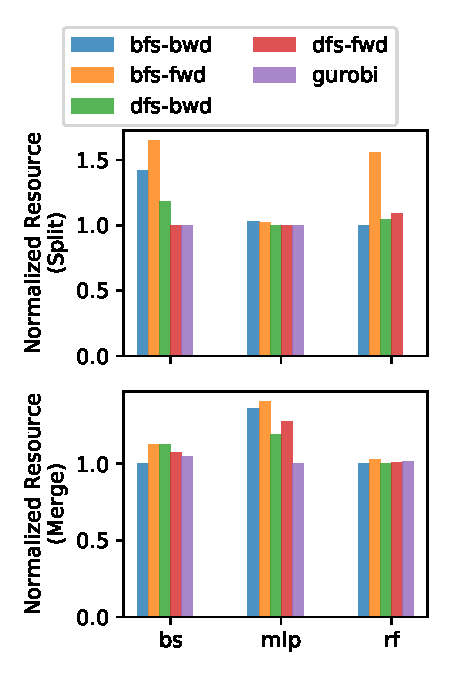
\includegraphics[width=1\textwidth]{figs/algo2.pdf}
\caption{Resource Comparison}
\end{subfigure}
\hfill
\begin{subfigure}[b]{0.64\textwidth}
\centering
\begin{tabular}{lccccc}
  \toprule
  Apps &bfs-bwd & bfs-fwd & dfs-bwd & dfs-fwd & gurobi \\ \midrule 
bs & 3s & 3s & 2s & 2s & 2h4m \\ 
mlp & <1s & <1s & <1s & <1s & 4s \\ 
rf & 1m37s & 1m7s & 29s & 27s & - \\ 

 \bottomrule
\end{tabular}
\caption{
  Compile time for spltting
}
\vspace{0.1cm}
\begin{tabular}{lccccc}
  \toprule
  Apps &bfs-bwd & bfs-fwd & dfs-bwd & dfs-fwd & gurobi \\ \midrule 
bs & 1s & 2s & 5s & 3s & 1m4s \\ 
mlp & 5s & 5s & 6s & 11s & 31m16s \\ 
rf & 11s & 10s & 2m7s & 1m0s & 14h27m \\ 

 \bottomrule
\end{tabular}
\caption{
  Compile time for merging
}
\vspace{0.65cm}
\end{subfigure}
\hfill
\caption[Partitioning and merging algorithm comparisons]{
  Partitioning and merging algorithm comparisons. (a) shows the normalized resource usage between
  different algorithms (the lower the better). (b) and (c) shows the compile time of each algorithm.
  Benchmarks include BlackScholes (bs), multi-layer perceptron (mlp), and random forests (rf).
}
\label{fig:split}
\end{figure*}

\Cref{fig:split} shows the comparison between the traversal-based and the solver-based solutions for both
compute partitioning and global merging.
Global merging is a global optimization merging small VUs into a large VU that can still fit in
a PU. 
The merging algorithm is very similar to the compute partitioning algorithm, where nodes in the
dataflow graph corresponds to the VUs in a VUDFG. 
The traversal and solver-based algorithms for partitioning can be extended to handle the merging
problem.
\Cref{sec:opt} will discuss merging problem in more detail.

We use a commercial solver, Gurobi~\cite{gurobi}, for the solver-based algorithm. 
The evaluation is performed on an Intel Xeon E7-8890 CPU at 2.5GHz with 1TB DDR4 RAM. 
Gurobi is parallelized across ten threads for each application.
To speed up convergence, we configure Gurobi with a 15\% optimality gap, i.e., 
the solver is allowed to early stop after the current solution is less than 15\% worse than the optimum
solution. 
%To speed up convergence, we use a 15\% optimality gap that stops the solver at a reasonable solution.
The solving time increases dramatically as getting close to 100\% optimum.

\Cref{fig:split} (a) shows the normalized resources in the number of VUs after partitioning and merging.
We can see that Gurobi provides almost the best solution for all applications when it can derive
an answer in a reasonable amount of time. The missing solver bar in random forest (\emph{rf}) partitioning
is due to timeout after a few days.
The traversal-based algorithms can sometimes match or even outperform the solver slightly.
However, because the partitioning result is a function of the traversal order, 
each traversal order has adversarial cases, where they can be up to 1.7x worse in resource than the best possible solution.
We found the forward (\emph{fwd}) traversal order schedules nodes as earlier as possible, reducing the number of
external live variables; the backward traversal minimizes the number of internal live variables
across partitions.
The depth-first-search (DFS) traversal order minimizes the number of live variables between partitions, 
albeit producing more imbalanced paths between partitions. 
On the other hand, breath-first-search (BFS) produces more balanced partitioning with more live variables and partitions.

There are two common graph patterns in the applications that require partitioning. 
The first is a dataflow graph from a large basic block, which contains a small set of external
live-in and -out variables and many intermediate temporary variables.
Such graphs typically end up with long-live variables across partitions that require retiming.
%\todo{show example and discuss the other pattern.}
The second is a balanced tree structure as the result of partitioning
a logical memory across PUs discussed later in \Cref{sec:memsplit}.
The first structure favors the DFS traversal order, minimizing the number of partitions. The second
structure favors the BFS traversal order, creating balanced partitions without additional
retiming VUs.

\Cref{fig:split} (b) and (c) shows the compile time for these algorithms. The single-threaded
the traversal-based algorithm runs in minutes, which is significantly faster than the parallelized solver that takes hours to days.
In general, the solver runtime becomes quickly unbounded with a large amount of VUs.
%\todo{show solver time with an increasing number of VBs}.

In summary, the solver solution provides a guaranteed close-to-optimum solution at an expensive
compile time. Nonetheless, the solver-solution treats the retiming and partitioning as a joint optimization,
whereas the traversal-based solution solves these two problems in two separate passes,
generating less optimal solutions.
Moreover, the solver-based solution tends to produce a better result for PUs with a tight I/O
bound (small number of I/Os and large number of stages).
The traversal-based solutions, on the other hand, can produce a decent solution in a short amount of
time.
However, the solution is a function of the traversal order; hence, the quality of the partitioning
is highly sensitive to the graph structures.
In practice, we can combine the two approaches and invoke the expensive solver only when the
traversal-based solution is insufficient. The quality of the traversal-based solution can be easily
estimated with the resource utilization of a partition.

\subsection{Memory Partitioning} \label{sec:memsplit}
The memory pruner addresses virtual on-chip memory exceeding the capacity and bandwidth limit of a
single PMU.
As we parallelize the computation, the on-chip memory must provide higher address bandwidth to sustain the
compute throughput.
On a processor-based architecture, this is often achieved with a separate first-level
cache for each processor core, as shown in \Cref{fig:memmodel} (a).
The cache implements a hardware coherence protocol that synchronizes the different copies of data
behind the scenes,
providing the abstraction of a shared memory.

\begin{figure}
  \begin{subfigure}[b]{0.35\textwidth}
  \centering
  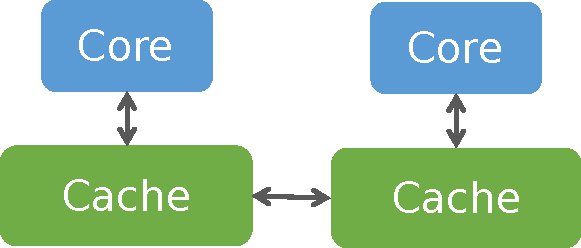
\includegraphics[width=1\columnwidth]{figs/cpumemmodel.pdf}
  \caption{Processor Architecture}
  \end{subfigure}
  \hfill
  \begin{subfigure}[b]{0.45\textwidth}
  \centering
  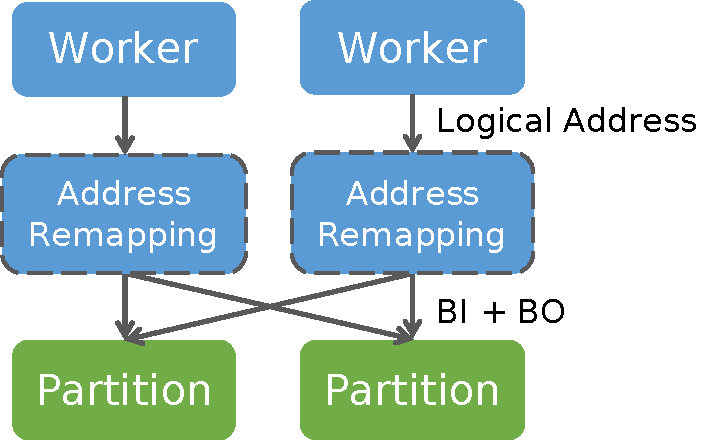
\includegraphics[width=1\columnwidth]{figs/spatialmemmodel.pdf}
  \caption{Reconfigurable Spatial Architecture}
  \end{subfigure}
  \caption[Memory model of different architectures]{Memory model of different architectures}
  \label{fig:memmodel}
\end{figure}
\begin{figure}
  \centering
  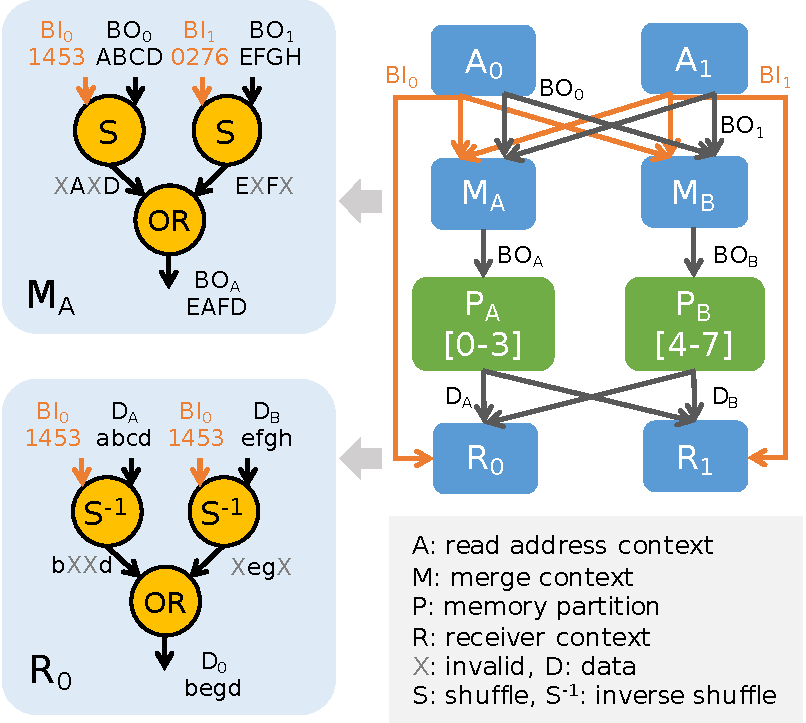
\includegraphics[width=0.6\columnwidth]{figs/memsplit2.pdf}
  \caption[Memory partitioning]{Example of memory partitioning across physical units. In this example, the program parallelizes the outer loop by two and vectorizes the inner loop by 4, which generates two vectorized access lanes. We need eight scratchpad banks to sustain the read bandwidth. 
  \name groups the 8 banks in two virtual memory partitions, $P_A$ (bank 0-3) and $P_B$ (bank 4-7). The address generation contexts $A_0$ and $A_1$ contains the computation for logical address and address remapping, which output $BA$s and $BO$s. \name allocates one merge context per memory partition
  ($M_A$ and $M_B$),
  merging requests from all access lanes. Inside the merge context, the shuffle operator converts the BO from access-aligned to bank-aligned. $A_0$, for example, requests offsets 
  A, B, C, and D ($BO_0$) from banks 1,4,5,and 3 ($BA_0$). The shuffle operator picks the requests belonging to partition A and outputs a BO aligned with bank 0-3. If the bank $i$ in the partition has no request, the $i$th element in the output is marked as invalid.
  The merge context contains one shuffle operator per request lane, and uses a tree of $OR$
  operators to combine all bank-aligned BOs into the final $BO_A$.
  On the receiver side, the memory broadcasts its response to all receiver lanes.
  The receiver context uses an inverse shuffle operator to convert the response from bank-aligned back to access-aligned, using the $BA$ forwarded from the address context. The response is then merged with another OR tree. 
  }
  \label{fig:memsplit}
\end{figure}

The coherence protocol is both expensive in hardware complexity and hard to scale in bandwidth for
streaming pipelined execution.
Instead of making redundant copies of the data, we can partition the data across different memory
partitions to get additional address port on a reconfigurable accelerator, as shown in
\Cref{fig:memmodel} (b).
Each parallel worker broadcasts the requests to all memory partitions.
If the data accessed by two parallel workers live in the same bank, the bandwidth will be halved.
To avoid bank conflicts, an important static analysis often used on reconfigurable accelerators is called static partitioning, or static banking~\cite{poly_cong}.
For most address patterns, the compiler can derive a partitioning scheme such that every partition is accessed by a
single worker at any time, which guarantees bandwidth at runtime.
The output of the analysis is an expression for bank address (BA) and bank offset (BO), both are
functions of the requested logical address.
BA determines which partition each request is going to, and BO is the offset within the
partition.

\Cref{fig:memsplit} shows how static banking is achieved on the Plasticine architecture.
Banking analysis from Spatial specifies the number of banks required to sustain bandwidth for the
current parallelization factors, and expressions for BAs and BOs. 
\name groups the banks into virtual memories, with group size limited by the number of banks in a PMU.
For each access lane, \name allocates a context to compute the logical and remapped address, which
outputs a vectorized BA and BO for each access lane. BAs and BOs are broadcasted to all memory partitions.
For each memory partition, \name allocates a merge context, merging BOs from all requesting lanes.
The merge context uses a shuffle operator to transform the vectorized BO from bank order specified by BA
(access-aligned) to bank order assigned to the current partition (bank-aligned).
Because the static banking analysis guarantees no bank conflicts for all banks,
\name can use a OR tree to merge the bank-aligned BOs into the final BO that gets send to
banks in the partition. On the receiver side, \name uses an inverse shuffle to convert responses from
partitions from bank-aligned back to access-aligned.
\name uses another OR tree to merge the access-aligned responses, which produces the final data
vector requested by the access lane.
With large parallelization, both the request OR tree and the respond OR tree can be
partitioned across VUs if running out of stages in a VU, scaling in the network bandwidth of the
crossbar connection by burning more VUs.

\Cref{sec:banking_arch} discusses the architectural changes to Plasticine to support this general
banking scheme.

\subsection{Register Allocation} \label{sec:regalloc}

After a VU is assigned to a PU, \name setups the configuration within a PU.
One of the configuration is assigning live variables in the dataflow graph to pipeline registers
across stages, shown in \Cref{fig:contexta}.

%\subsubsection{Blackbox IP Pruning} \label{sec:bbsplit}
%\yz{Cut this if out of the space}
%This step illustrates an example of integrating a customized partitioner for composable IP available on
%the architecture.
%The cost metrics and partition rule are specific to each IP.
%The example IP is a merge buffer, which can merge two sorted vector streams into a single stream with
%one vector per cycle throughput.
%The merge buffer pruner uses a tree of 2-way merge buffers across PUs to compose a multi-way merge buffer declared in the program.

\section{Optimizations}\label{sec:opt}
\name performs many of the standard compiler optimizations,
such as Dead Code Elimination and Constant Propagation.
Some of them, however, plays a much more important rule for reconfigurable accelerator because they
have direct impact on the resource usage.
Other optimizations can be counter-intuitive, as they introduce redundant computation that
reduces resource without necessarily impacting performance.
In this discussion, we focus our primary objective on performance.
Resource is an indirect objective as resource reduction enable larger parallelization factors,
, which in turn improves performance.

\subparagraph{Memory strength reduction (msr).} Like traditional strength reduction on arithmetics, \name{} replaces expensive on-chip memories with cheaper memories whenever possible.
%We map register accumulation in the program with single-cycle initiation interval to pipeline registers.
For example, \name{} replaces a scratchpad with constant address in all accesses to a un-indexable memory, such as a FIFO.
This commonly happens when producer and consumer loops of the memory are fully unrolled.

\subparagraph{Route-Through Elimination (rtelm).} For patterns where the content of a non-indexable memory  (M1) is read and written to another memory (M2), \name{} eliminates the intermediate access if the read of M1 and the write of M2 operates in lock-step.

\begin{figure*}
\centering
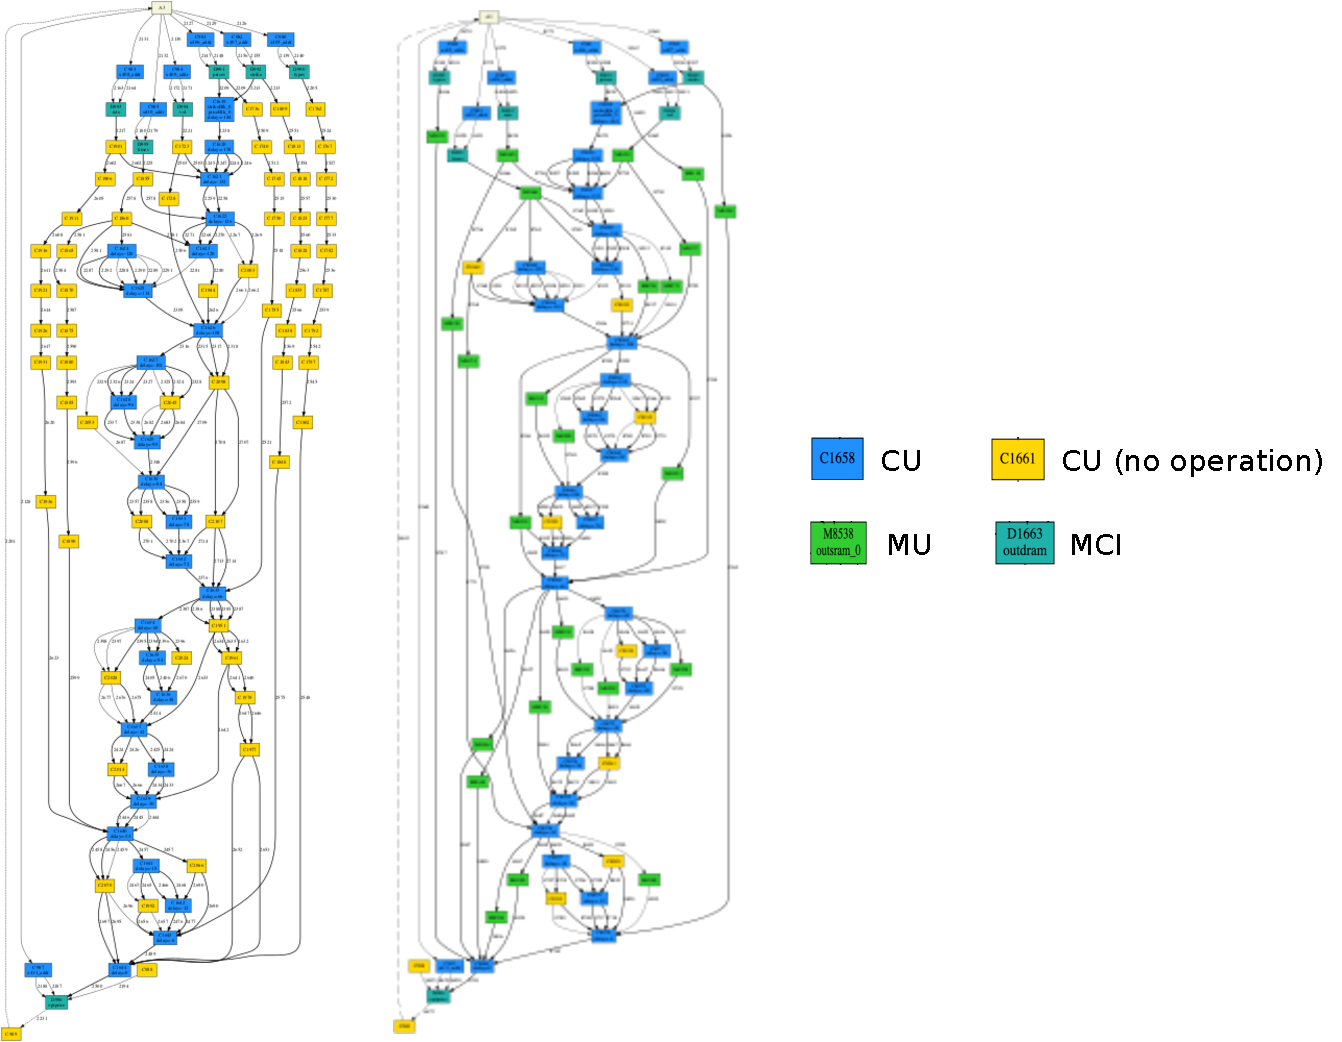
\includegraphics[width=0.7\textwidth]{figs/retiming.pdf}
\caption[Retiming]{
  Left: retiming with input buffer only. Right: retiming with either input buffer or scratchpad.
}
\label{fig:mlp}
\end{figure*}
\subparagraph{Retiming with scratchpad (retime-mem).} By default, \name{} uses PB input buffers for retiming purpose. 
This option enables \name{} to use scratchpad memory for retiming that requires large buffer depth.

\subparagraph{Crossbar datapath elimination (xbar-elm).}
Although, crossbars between accessors and memory partitions (\Cref{sec:memsplit}) are very expensive in the general case, the BI sometimes can be statically resolvable with certain combinations of parallelization on memory accesses. 
When BI is a constant, \name{} can use this information to intelligently assign virtual banks to partitions that reduce the crossbar data path to a partial or a point-to-point connection.

\subparagraph{Read request duplication (dupra).} During memory partitioning (\Cref{sec:memsplit}), instead of forwarding BI from the requester to receiver, \name{} can also duplicate the BI with local state on receiver side, which
eliminates the unbalanced data path at the cost of extra computation.

\begin{figure*}
\centering
\begin{subfigure}[b]{0.6\textwidth}
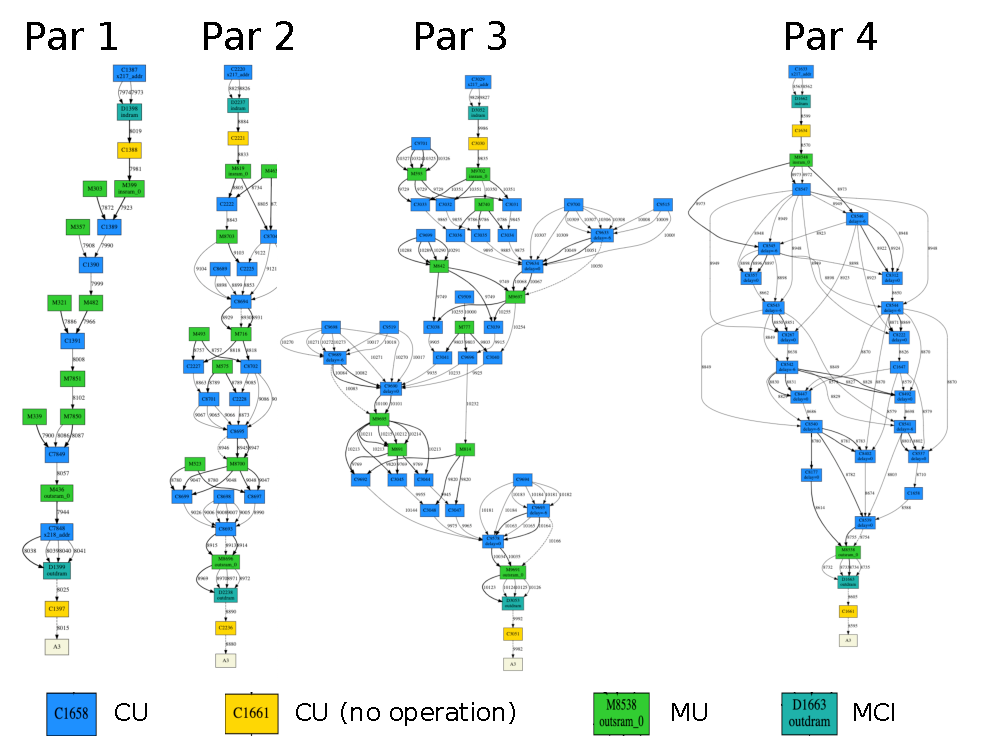
\includegraphics[width=1\textwidth]{figs/mlpunroll.pdf}
\caption{VUDFGs with different parallelization factors}
\end{subfigure}
\hfill
\begin{subfigure}[b]{0.39\textwidth}
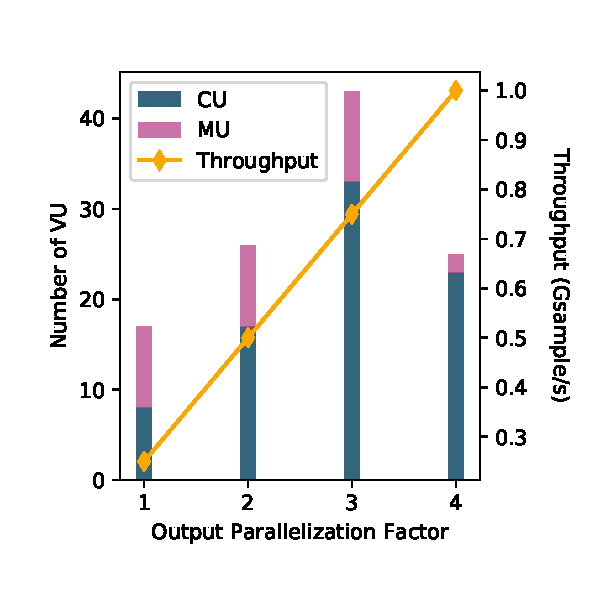
\includegraphics[width=1\textwidth]{figs/mlp.pdf}
\caption{Throughput and resource as a function of parallelization factor}
\end{subfigure}
\caption[MLP case study]{
  MLP case study
}
\label{fig:mlp}
\end{figure*}

\subparagraph{Global Merging (merge).}
After all VBs satisfy the hardware constraint, we perform a global optimization to compact small VBs into  larger VBs. 
Merging has very similar problem statement as compute partitioning (\Cref{sec:compsplit}) except with more constraints.
The traversal-based algorithm requires a reference cost for PB to check if the merged VB still satisfy the hardware constraint.
At each step of merging, we take the union of the domains of VBs within the current partition, and intersect with the domain of the merging VB.
The caveat is that even with a non-empty intersection, the bipartite graph might not have a possible assignment, as merged VB might fit in a larger PB with insufficient quantity.
Therefore, we perform a heuristic checking on feasibility of the bipartite assignment at each step of merging.
The solver-based solution combines partition assignment with PB type assignment as a joint problem. 
The output of merging gives both partition assignment as well as a PB type assignment, which eliminates the risk of un-mappable bipartite graph due to merging in the traversal-based solution.

\subparagraph{Memory Localization}
We perform another specialization on non-indexable memories (registers or FIFOs), whose all accesses have no explicit read enables.
Instead of treating them as shared memories, \name{} duplicates and maps them to local input buffers in all receivers, no longer requiring tokens.
The sender actor pushes to the network when the token is supposed to be sent, and the receiver dequeues one element from the input buffer when the token is supposed to be consumed.
This dramatically reduces the synchronization complexity of non-indexable memory in the common case.

\subparagraph{Reverse Loop Invariant Hoisting}
A common loop optimizations is to move loop invariant expressions outside of the loop body to reduce
computation. This optimizations, however, might introduce more basic blocks in the program.
For Plasticine, number of basic blocks have a strong correlation with number of contexts and
physical units. \Cref{fig:reversehoisting} shows an example where moving instructions into the loop
body reduces number compute units. Because instructions within basic blocks and basic blocks
themselves are pipelined, doing so does not have performance impact on the application.
Currently, we rely on the user to perform manually perform this optimization.

\begin{figure*}
\centering
\hfill
\begin{subfigure}[b]{0.4\textwidth}
\inputminted{python}{code/hoisting.py}
\caption{Input program}
\end{subfigure}
\hfill
\begin{subfigure}[b]{0.4\textwidth}
\inputminted{python}{code/reversehoisting.py}
\caption{Reverse Loop Invariant Hoisting}
\end{subfigure}
\hfill
\caption[Reverse Loop Invariant Hoisting]{
  The original program requires at least two contexts to execute Block 1 and Block 2.
  By moving the invariant instruction \texttt{c = a + b} into the loop body, (b) only needs a single
  context instead. Because instructions within \texttt{Block 2} are pipelined across loop
  iterations, adding instructions in the loop body introduce minimum performance impact.
  This transformation is beneficial until \texttt{Block 2} exceeds six operations, at which point
  both version consume the same amount of resources.
}
\label{fig:reversehoisting}
\end{figure*}

\begin{figure*}
\centering
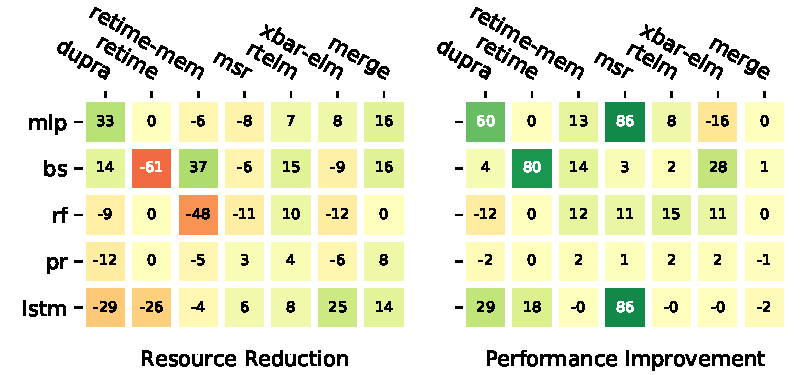
\includegraphics[width=0.7\textwidth]{figs/heat.pdf}
\caption[Optimization Effectiveness]{
  Optimization Effectiveness. Percentage resource reduction or performance improvement from each
  optimization. The heat map shows the maximum differences when turning on/off the optimization, 
  while keeping other optimizations the same.
  For a single application, the improvement is taking the geometric mean across different application parameters.
}
\label{fig:reversehoisting}
\end{figure*}

\begin{figure*}
\centering
\hfill
\begin{subfigure}[b]{0.35\textwidth}
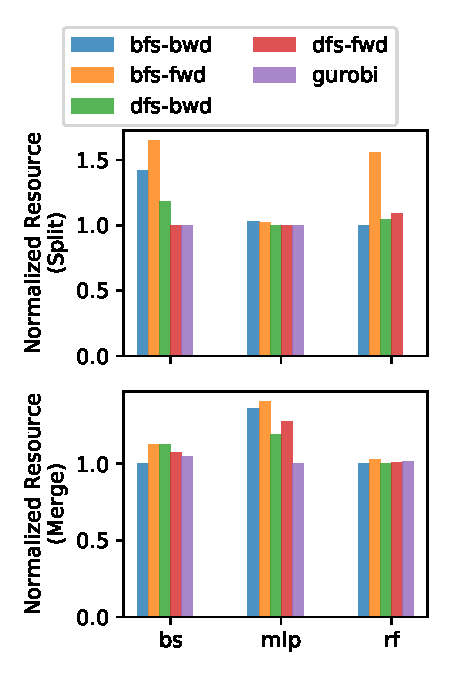
\includegraphics[width=1\textwidth]{figs/algo2.pdf}
\caption{Resource Comparison}
\end{subfigure}
\hfill
\begin{subfigure}[b]{0.64\textwidth}
\centering
\begin{tabular}{lccccc}
  \toprule
  Apps &bfs-bwd & bfs-fwd & dfs-bwd & dfs-fwd & gurobi \\ \midrule 
bs & 3s & 3s & 2s & 2s & 2h4m \\ 
mlp & <1s & <1s & <1s & <1s & 4s \\ 
rf & 1m37s & 1m7s & 29s & 27s & - \\ 

 \bottomrule
\end{tabular}
\caption{
  Compile time for spltting
}
\vspace{0.1cm}
\begin{tabular}{lccccc}
  \toprule
  Apps &bfs-bwd & bfs-fwd & dfs-bwd & dfs-fwd & gurobi \\ \midrule 
bs & 1s & 2s & 5s & 3s & 1m4s \\ 
mlp & 5s & 5s & 6s & 11s & 31m16s \\ 
rf & 11s & 10s & 2m7s & 1m0s & 14h27m \\ 

 \bottomrule
\end{tabular}
\caption{
  Compile time for merging
}
\vspace{0.65cm}
\end{subfigure}
\hfill
\caption[Partitioning and merging algorithm comparison]{
  Partitioning and merging algorithm comparison. (a) shows the normalized resource usage between
  different algorithms (the lower the better). (b) and (c) shows the compile time of each algorithm.
}
\label{fig:split}
\end{figure*}
%\subparagraph{Dead Code Elimination (DCE)} 
%We perform aggressive DCE on the VBDFG and only keeps computation that gets materialized to accelerator I/O and DRAM.
%\subparagraph{Constant Propagation}
%Aside from regular constant propagation on arithmetics, we also eliminates crossbar datapath when bank ID 
%can be statically resolved described later in \Cref{sec:memsplit}.
%During loop unrolling, address of indexable memory sometimes can be resolved to static constant.
%For a read-only RAM with constant address, we lookup their content at compile time and embed its content into registers.
%For \emph{route-through} pattern, where content of a non-indexable memory M1 is read and written to another memory M2,
%we can eliminate the intermediate write and forward the data directly to the final memory if the compiler
%can prove the read M1 and write of M2 operates in lock-step.
%We also perform constant propagation on control signals with loop-range analysis. 
%Eliminates the control signals can expose more lock-step accesses and \emph{route-through} opportunities.
%\subparagraph{Strength Reduction}
%In addition to traditional strength reduction on arithmetics, we also replace expensive memories
%with cheaper memory whenever possible.
%We map register accumulation in the program with single-cycle initiation interval to pipeline registers.
%Banked-SRAM with constant bank IDs and offsets in all accessors can also be replaced with FIFOs,
%which is happens when producer and consumer loops are fully unrolled.

%Accesses statically banked in the input graph can operates concurrently 
%without bank conflicts, as explained in \Cref{sec:background}.
%These accesses are usually from a unrolled loops. For banked accesses from the same pre-unrolled access, 
%\name first merge all requests before sending to the memory (details in \Cref{sec:memsplit}). 
%Because these accesses are from loop unrolling, they have the same program order and same dependency with other accesses.
%So the synchronization can be performed on the merged access, which prevents the amount of synchronization
%to increase with parallelism on a banked memory, as shown in \Cref{fig:mergetoken}

%\subsubsection{Blackbox IP Pruning} \label{sec:bbsplit}
%\yz{Cut this if out of the space}
%This step illustrates an example of integrating a customized partitioner for composable IP available on
%the architecture.
%The cost metrics and partition rule is specific to each IP.
%The example IP is a merge buffer, which can merge two sorted vector streams into a single stream with
%one vector per cycle throughput.
%The merge buffer pruner uses a tree of 2-way merge buffers across PBs to compose a multi-way merge buffer declared in the program.



\section{Placement and Routing} \label{sec:par}
The input to the \emph{placement and routing (PaR)} phase is a VUDFG, with each VU tagged to a PU
type.
Before PaR, \name also performs a runtime analysis of the program, annotating each edge in the VUDFG
with a link priority. The link priority is used to determine the routing order during PaR.
PaR then iteratively places VUs and route edges in VUDFG onto the global network.

In addition to the original static network in Plasticine, we introduce a dynamic network in
parallel to the static network, forming a dynamic-static hybrid network.
Both purely static and purely dynamic networks are instances of the parameterized hybrid network.
\Cref{sec:network} will discuss the details about the hybrid network.
The PaR algorithm needs to handle both network types and multiple network granularity (vector,
scalar, control) at the same time.

The major difference between the static and the dynamic network is that each physical link in the static network is dedicated to a logical edge in the VUDFG for the entire duration of the execution
(circuit-switching\footnote{Technically, our static network is more restrictive than
circuit-switching because circuit-switching allows deallocation after the connection is terminated.
Our static network, on the other hand, cannot be reconfigured until the application terminates.}), whereas 
the physical link in the dynamic network can be time-shared by multiple logical edges
(packet-switching).
Both static and dynamic networks are statically routed by the PaR algorithm. 
For a dynamic network, PaR also needs to assign virtual channels (VCs) to prevent network deadlock.
The PaR algorithm configures the lookup table in each router that maps the packet header to the
destination port and VC.

In the rest of this section, \Cref{sec:place} and \Cref{sec:route} discusses the placement 
and the routing algorithm. 
\Cref{sec:vc} explains the need for VC allocation. 
Lastly, \Cref{sec:heuristic} describes how \name generates link priority.

\subsection{Iterative Placement} \label{sec:place}

At high-level, the PaR algorithm works very similarly to the FPGA PaR using
simulated annealing~\cite{simanneal}. 
For the initial placement, the algorithm places VUs in VUDFG in topological order.
Each VU is placed to the next available PU with minimum Manhattan distance to the placed
neighbors of that VU.
Next, the algorithm routes all edges in the VUDFG, starting from edges with the highest link
priority. If no routes are available on the static network, the route will be moved onto the dynamic
network. For purely static networks, there is an ``imaginary'' dynamic network for this step.
If there are still routes on the fake dynamic network at the end of the PaR, PaR is considered
failed for the purely static network.
After all routes are routed, either on the static or dynamic network, the PaR evaluates the
congestion cost of the current placement.
Then, a genetic algorithm shuffles the VUs whose edges contribute most to congestion, 
and keeps the new position if it improves the route assignment.
By iteratively re-placing and re-routing, the mapping process eventually converges to a good placement.

The PaR uses a heuristic cost model to rapidly evaluate placements: a 
penalty score is assigned as a linear function of several subscores.
These include projected congestion on dynamic links, projected congestion at network injection and ejection ports, the average route length, and the length of the longest route.
\name provides a static estimate of the number of packets sent on each logical link.
The PaR algorithm estimates congestion by normalizing the number of packets on each link to the program link with the highest total packet count.
The most active program link sets a lower bound on the program runtime (the highest bandwidth physical link can still only send one packet per cycle), which translates to an upper bound on congestion for other links.

%The {\sc Unplace} function randomly decides between unplacing a random node, and unplacing one or several nodes based on heuristics.
%For the heuristic-based unplacement, a node's contribution to global route congestion is calculated by adding an estimate of all connected routes' contributions to the global penalty score; the node(s) with the highest scores are unplaced.
%Similarly, {\sc Place} also can either randomly place an unplaced node, or place it to minimize the Manhattan distance to its logical neighbors. {\sc Score} calculates the heuristics for each node, and {\sc Filter} duplicates the best candidate placements to fill the pool. Because the unplacement and replacement steps can make a placement worse, the best performing placements are frozen in each iteration to ensure that no good placements are thrown away.

\subsection{Congestion-Aware Routing} \label{sec:route}
%\info{Somewhere we should mention that placement and routing running interchangeably}
To achieve optimal performance, we use a routing algorithm that projects congestion and routes around it. 
Routing starts with the highest-priority routes, as determined by fanout of the broadcast edge and
estimated packet count; broadcast edge with higher fanout is harder to route and hence are routed
first.
Using the packet count as a priority makes sure that the static network is used most efficiently.
Our scheme searches a large space of routes for each link, using Dijkstra's algorithm \cite{dijkstra} and a hop weighting function.
To ensure maximum link reuse in broadcast edges, we can augment the hop weight in Dijkstra's
algorithm by a multiplication factor between zero and one. 
When finding the shortest path between each source-destination pair, the weight of the hop is
multiplied by the factor each time the hop is reused for the same broadcast edge.
In other words, the reused path has a lower hop cost compared to other paths.
This trick provides a balance between the shortest path and link reuse: a smaller factor encourages link
reuse, even though individual source-destination pairs are not the shortest path; a factor equals to 1 ensure all source-destination pairs are routed with the shortest path.
The second objective for routing broadcast links is balancing the hop counts between all
destinations. This is because the shorter path will back pressure the sender before packets reaching to the longer path, causing pipeline stalls.
To achieve this, we start with the source-destination pair with the longest Manhattan distance, ensuring
the most far apart source-destination pair is routed on the shortest path.
The consecutive source-destination pairs will try sharing the link on this path and slightly detour from
their shortest path, which balances the hop count.
%Routes are not analyzed on the basis of a single source-destination pair, which would be inadequate for broadcasts: instead, a directed graph is built from the source and all destinations in the route, with edge weights corresponding to the minimal route between each pair of VUs in the broadcast.
%For example, if the broadcast is from VU-1 to VU-2 and VU-3, four total potential routes are analyzed for congestion: VU-1 to VU-2, VU-1 to VU-3, VU-2 to VU-3, and VU-3 to VU-2.
%The routes are weighted so that routes mapped on the static network are preferable to those mapped to the dynamic network; within these categories, routes are weighted based on length. 

%\info{does the nodes refer to only source and destinations or including all nodes on the path between source and destination. How does the weights represent the minimum routes? Is it capturing the cost of the minimum route?}
%Then, a search algorithm based on Prim's algorithm for minimum spanning trees \cite{prim1957shortest} is run to build a tree for the broadcast, starting with only the source being reached.
%At every step, the most-preferable route (from the graph built using Dijkstra's algorithm) that adds a new destination VU to the reached set is chosen and added to the broadcast, until all destination VUs are reached. 
%This route can start from either the source of the broadcast tree or any destination currently in the reached set.
%The algorithm will find a fully static broadcast tree, if one exists, and will only add a non-static route to the broadcast (moving the entire broadcast to the dynamic network) when there are VUs in the tree that cannot be reached from the source VU by \emph{any} static route.
%\info{does the algorithm routes links from high priority to low from all nodes or it does one node at a time?}

\subsection{VC Allocation for Deadlock Avoidance} \label{sec:vc}
Deadlock is a system pathology in dynamic routing where multiple flits form a cyclic holds on/waits for dependency on each others' buffers and prevent forward progress.
Most dataflow accelerators use a streaming model, where outputs of a producer are sent over the network to one or more consumers
without an explicit request; the producer is backpressure when there is insufficient buffer space. 
While this paradigm improves accelerator throughout by avoiding the round-trip delay of a request-response protocol, it introduces an additional source of deadlock \cite{hansson2007avoiding}. 

\Cref{fig:deadlock}(a) shows a sample VUDFG graph, which is statically placed and routed on a $2\times3$ network in (b). 
Logical edges B and C share a physical link in the network. If C fills the buffer shared with B, VU-3 will never receive any packets from B and will not make forward progress.
%For y-z dimension-order routing, the only valid routes from VU-1 to VU-3 is through $\[0,1\], \[0,0\], \[1,0\], \[2,0\]$. 
%Dimension-order routing prevents deadlock by eliminating cycles in network routes.
%On traditional NoCs, deadlock can be solved with dimension-order routing, which routes all traffic on one dimension before another.
%\yaqi{
  With streaming computation, the program graph must be considered as part of the network dependency graph, which must be cycle-free to guarantee deadlock freedom. However, this is infeasible because cycles can exist in a valid VU dataflow graph when the original program has a loop-carried dependency. Therefore, deadlock avoidance using cycle-free routing, such as dimension-order routing, does not work in our scenario. 
Allocating VCs to prevent multiple logical links from sharing the same physical buffer is consequently the most practical option for deadlock avoidance on streaming accelerators.
%Because the entire program is connected through these streaming dependencies, any two links can conflict and result in a deadlock.
%\yaqi{However, cycles are permitted in the programming paradigms since loop-carried dependencies can be mapped across the network.
%Therefore, we perform VC allocation at each router to prevent multiple logical links from sharing the same physical buffer.
\if 0
Virtual channel (VC) allocation is another common approach to avoid deadlock. We can statically assign conflicting streams B and C with different
virtual channels at router $[2,0]$, which prevents them to share physical buffers. 
Notice indirect inputs of a VU, such as A and D with eventual consumer VU-3,
also need distinct VCs to ensure deadlock-free. To minimize the number of VCs required, we perform per-hop VC allocation--statically
assign conflicting links at each input of each router with distinct VCs. The VCs can be looked up at runtime based on link ID.
Distinct links from the same source VU, such as A and C, can share the same VC because VU-1 ensures the number of flits sent over A and C remains
to a ratio that the receiver expects, which permits data to drain in the network.
\fi

\begin{figure}
\centering
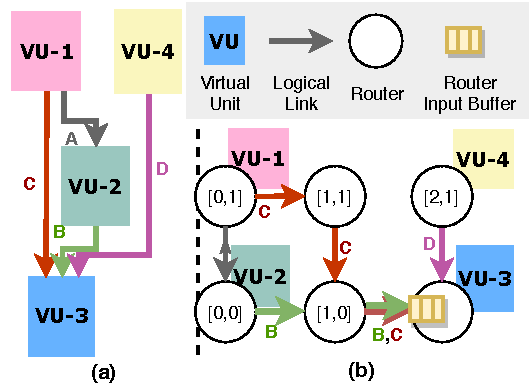
\includegraphics[width=0.4\columnwidth]{figs/deadlock.pdf}
  \caption[Network deadlock in streaming accelerators]{An example of deadlock in a streaming accelerator, showing the (a) VU data-flow graph and (b) physical placement and routes on a $2\times3$ network. There are input buffers at all router inputs, but only the buffer of interest is shown.}\small\textsuperscript{}\label{fig:deadlock}
\end{figure}

\subsection{Runtime Analysis for Heuristic Generation} \label{sec:heuristic}

In Spatial, users can annotate the value of runtime variables to assist compiler analysis.  
We use these programmer annotations to compute the expected number of iterations each basic block
will execute. 
The execution count on the basic block can further be used to derive the packet counts produced
by these basic blocks.
For a loop with data-dependent bounds, the user can annotate an estimate of the bound value.
For a branch statement, the user can annotate a percentage distribute between the if and else clauses.
The runtime of a streaming program is a function of the number of packets received on the incoming
stream. 
Static runtime analysis can identify potential application-level deadlock due to stream mismatching, as shown
in \Cref{fig:runtime}.

The derived packet counts based on these annotations can help the placer to evenly spread out the traffic.
The placer prioritizes highly used links on the static network and leaves infrequently used links on the dynamic network. 
However, we do not require exact annotations for efficient placement---rough estimates of these runtime values are sufficient to determine the relative importance of links.
When no annotation is provided, the compiler estimates
loop iteration counts based on the nesting depth: packets generated by the innermost loops are 
the more likely to be frequent.
This heuristic provides a reasonable estimate of links' priorities for routing purposes.

\begin{figure*}
\centering
\begin{subfigure}[b]{0.8\textwidth}
\inputminted{python}{code/runtime.py}
\caption{Example program}
\end{subfigure}
\caption[Runtime analysis]{
  Example of a streaming program whose runtime depends on the number of packets received on
  \texttt{stream}. We use a \texttt{queue} to model a stream receiving the packets from the
  network.
  Loop \emph{A} is a forever loop whose runtime is determined by its child controllers.
  With user annotation on number of packets from \texttt{stream}, 
  we know the runtime of loop \emph{B} is $T(B) = N$.
  As a result, we can derive the runtime of loop \emph{B}'s and parent \emph{A}, 
  i.e. $T(A) = \lceil\frac{N}{B}\rceil$. 
  With runtime for $A$, the runtime for $C$,$D$,and $E$ can be computed as
  $T(C) = \lceil\frac{N}{B}\rceil\cdot C$,
  $T(D) = \lceil\frac{N}{B}\rceil\cdot C \cdot R$, 
  and $T(E) = \lceil\frac{N}{B}\rceil\cdot C \cdot R \cdot E$.
  The runtime for \emph{E} also depends on \texttt{q}, which gives $T(E) = T(B) = N$. 
  If $\lceil\frac{N}{B}\rceil\cdot C \cdot R \cdot E \neq N$, \name gives an warnning for the
  inconsistency that potentially triggers an undesired deadlock.
}
\label{fig:runtime}
\end{figure*}

%\section{Debugging and Instrumentation Support (WIP)}
%\subsubsection{Deadlock in Streaming Reconfigurable Architecture}

%\subsubsection{Debugging Support and Performance Instrumentation}

\section{Evaluation (WIP)} \label{sec:eval}

\begin{figure*}
\centering
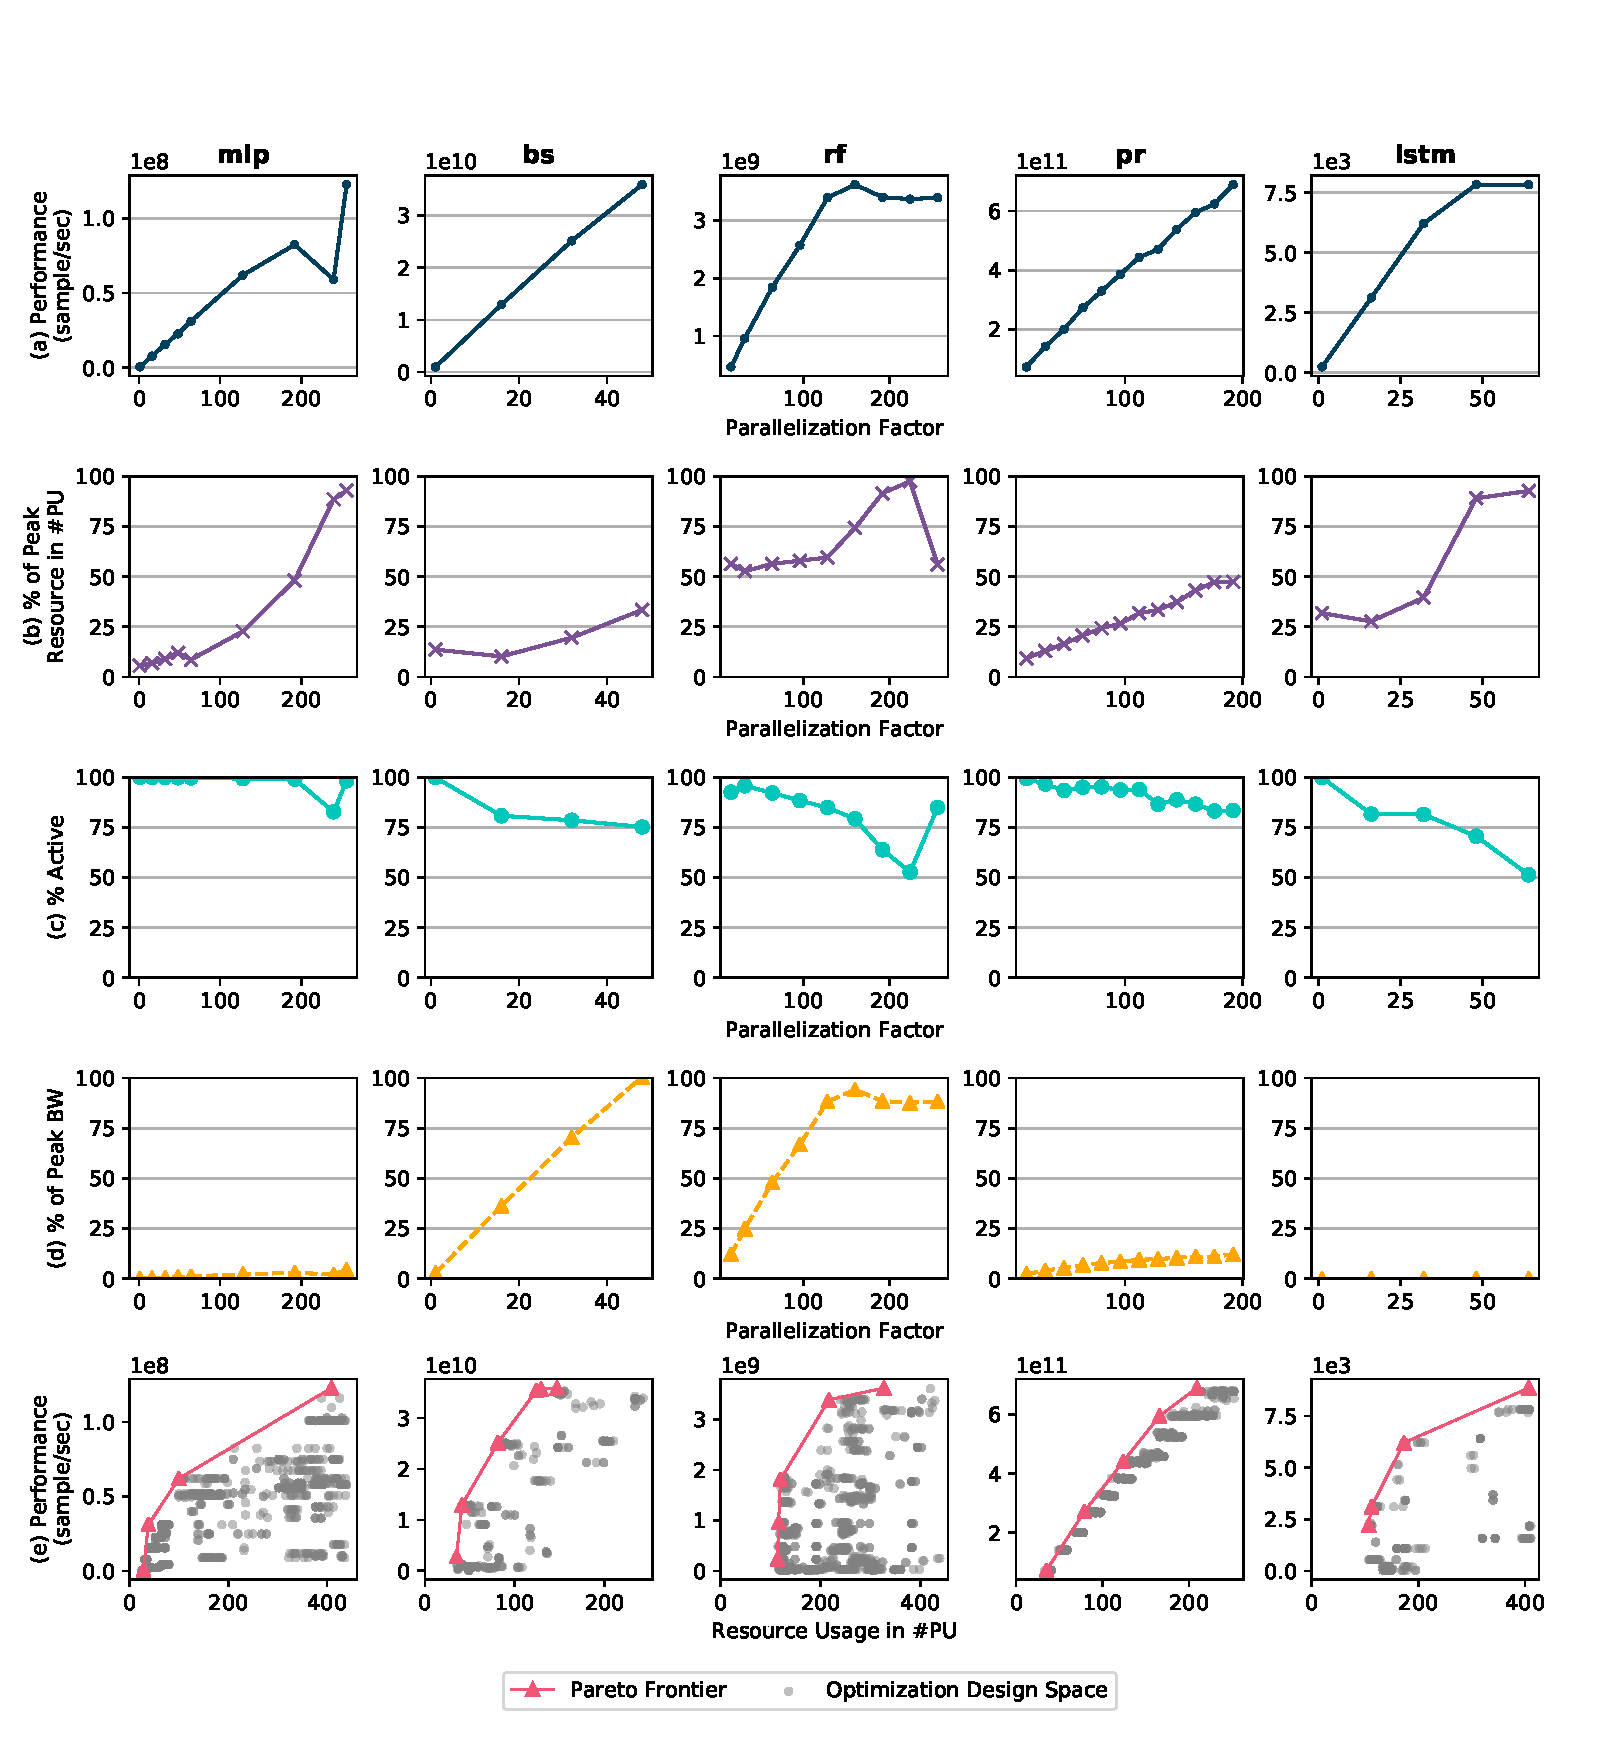
\includegraphics[width=1\textwidth]{/Users/yaqiz/pldi20/paper/figures/par_thesis.pdf}
\caption[Scalability Evaluation]{
  Scalability Evaluation. 
  The first four charts show the scaling of
  (a) throughput, 
  (b) resource usage, 
  (c) runtime activation rate of PUs on the critical path of the compute pipeline, 
  and (d) achieved HBM bandwidth, as the program gets parallelized.
  (e) shows the combined design space of compiler optimizations and parallelization factors on a
  throughput-resource curve. 
  The pareto frontier presents the throughput shown in (a) as a function of resource increase in
  (b).
}
\label{fig:par}
\end{figure*}

%\begin{figure*}
%\centering
%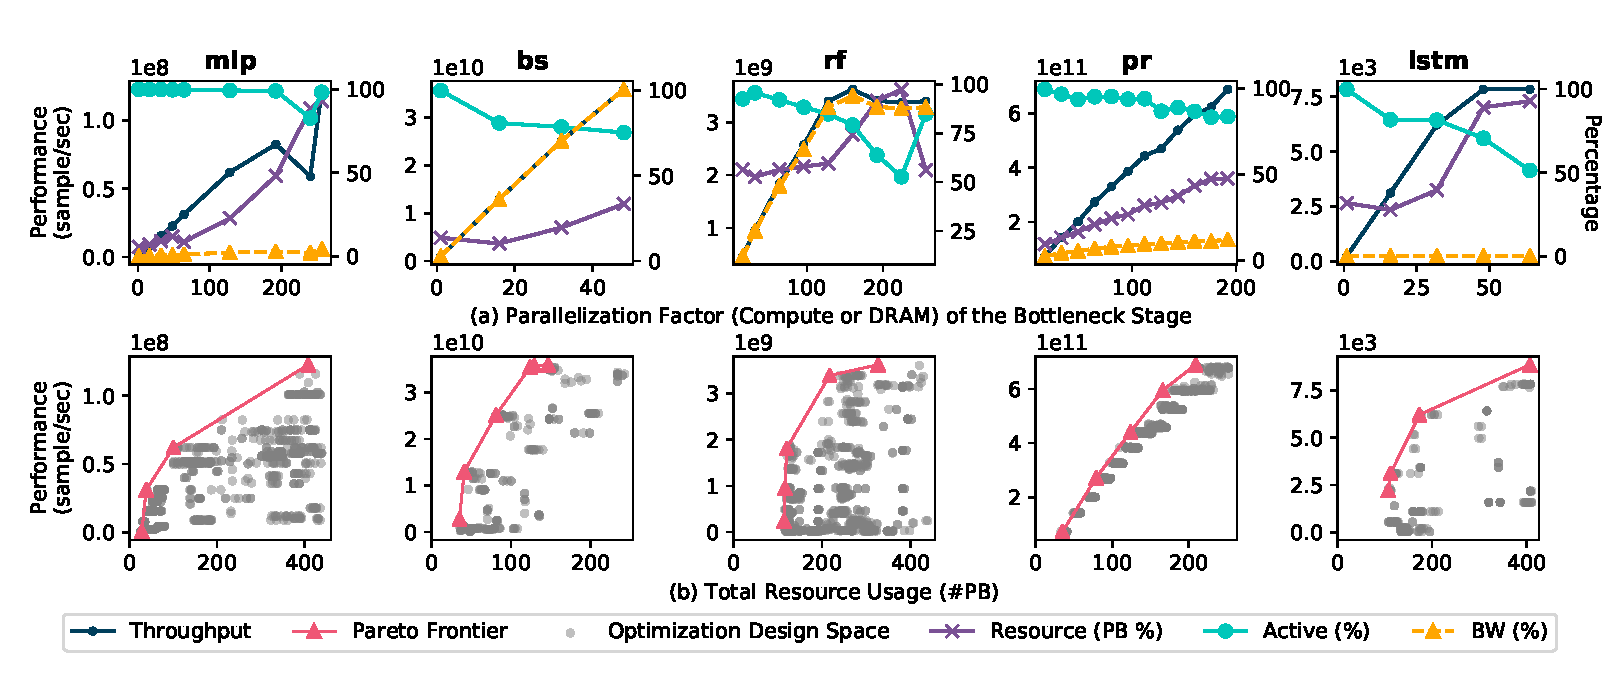
\includegraphics[width=1\textwidth]{/Users/yaqiz/pldi20/paper/figures/par.pdf}
%\caption[Performance comparison with V100 GPU]{
%}
%\label{fig:par}
%\end{figure*}

\begin{table}[t]
  \centering
    \footnotesize
    \begin{tabular}{lcccccc}
    \toprule
      \multirow{2}{*}{\textbf{Benchmark}} &
      \multirow{2}{*}{\makecell[c]{\bf Throughout\\\bf Unit}} &
      \multirow{2}{*}{\makecell[c]{\bf GPU\\\bf Compiler}} & \multicolumn{2}{c}{\textbf{Latency} (ms)} &
      \multicolumn{2}{c}{\textbf{Throughput} (Unit/s)} \\
                                & & & \name & GPU & \name & GPU     \\
      \midrule
        SqueezeNet (batch-1) & {\em kFrames}   & TF+cuDNN & 49.13  & 70.10  & 0.12 (1.1) & 0.4   \\ \addlinespace
        LSTM (batch-32)      & {\em kSamples}  & TF+cuDNN & 3.61   & 6.81   & 8.8 (79.2) & 4.7   \\ \addlinespace
        PageRank             & {\em MEdges}    & GunRock & 128.27 & 829.39 & 49         & 7.5   \\ \addlinespace
        BlackScholes         & {\em GOptions}  & CUDA & 0.09   & 0.10   & 88.88      & 80.02 \\ \addlinespace
        Random Forest        & {\em MSamples}  & CUDA & 0.10   & 0.32   & 1.04       & 0.32  \\ \addlinespace
        Merge Sort           & {\em GElements} & CUDA & 0.63   & 2.14   & 6.65       & 1.96  \\
      \bottomrule
    \end{tabular}
  \caption{Performance comparison of Plasticine with Tesla's V100 GPU (Normalized throughput to transistor count in parentheses).}
  \label{tab:gpu-comparison}
\end{table}
\begin{figure*}
\centering
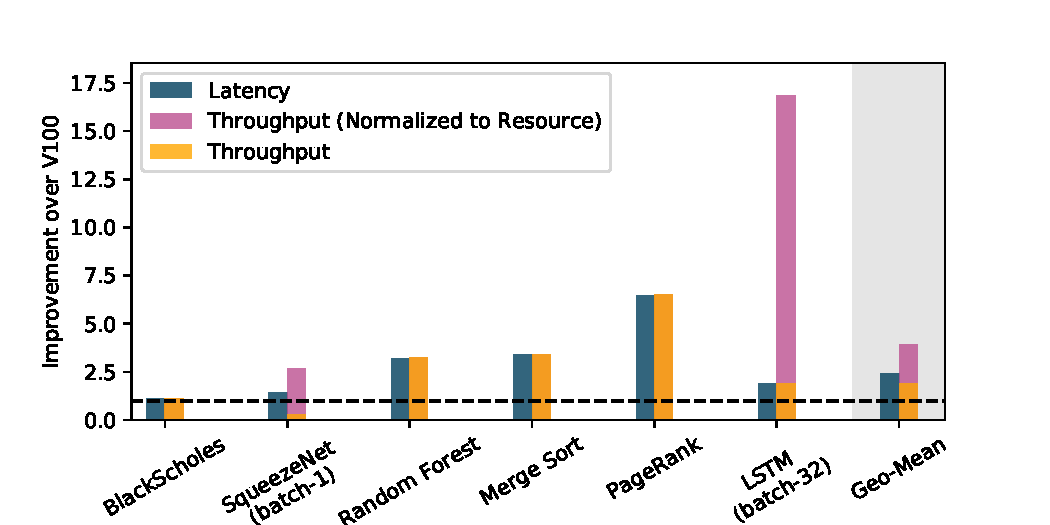
\includegraphics[width=1\textwidth]{figs/slide_gpu.pdf}
\caption[Performance comparison with V100 GPU]{
  Plasticine's latency and throughout improvement over V100 GPU.
  The evaluated Plasticine architecture has area footprint of 352$mm^2$ at 28nm.
  V100 GPU has area footprint of 815$mm^2$ at 12nm.
  Both platforms have the same off-chip bandwidth at 1TB/s with HBM technology.
  Yellow and blue bars show the raw measured speedup in throughput and latency, respectively.
  To account for the resource discrepancy, the pink bar shows the normalized throughput
  for compute-bound application--SqueezeNet and LSTM, which scales performance with additionally
  on-chip resources.
}
\label{fig:peakutil}
\end{figure*}



%\chapter{Architecture} \label{sec:arch}

In this section, we discuss the architectural advancement on top of the original Plasticine architecture
introduced in~\cite{plasticine}. These architectural additions help increase the application
coverage or improve the mapping strategies of existing applications by supporting new language
constructs, data types, and improves the utilization of the hardware. 
Specifically, \Cref{sec:banking_arch} layouts the datapath changes in order to support more
flexible banking schemes required by general access patterns supported in Spatial; 
\Cref{sec:rnn_arch} discusses the hardware specialization and architectural sizing for machine
learning applications; \Cref{network} provides an extensive study on on-chip network selection 
reconfigurable spatial architectures.

\begin{figure*}
\centering
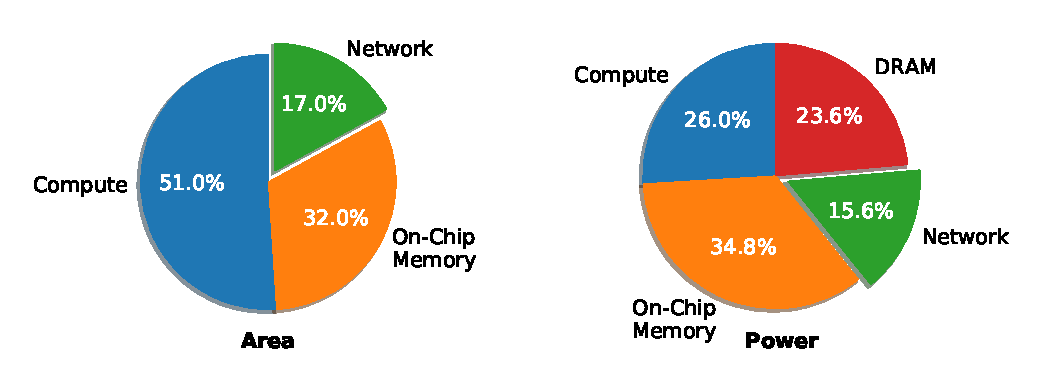
\includegraphics[width=1\textwidth]{figs/pie.pdf}
\caption[Area and power breakdown of Plasticine]{
  Area and power breakdown of Plasticine
}
\label{fig:breakdown}
\end{figure*}

\section{On-chip Network} \label{sec:network}

Achieving scalable performance using spatial architectures while supporting diverse applications requires a flexible, high-bandwidth interconnect.
  %Unfortunately, bandwidth and flexibility are often conflicting goals; static interconnects guarantee bandwidth but lack flexibility due to poor sharing.
  %Dynamic interconnects provide flexibility with better resource sharing but can cause bandwidth bottlenecks due to congestion while requiring more area and power.
 Because modern RDAs support vector units with wide datapaths, designing an interconnect that balances dynamism, communication granularity, and programmability is a challenging task.

On-chip interconnects can be classified into two broad categories: \emph{static} and \emph{dynamic.}
 {Static interconnects} use switches programmed at compile time to reserve high-bandwidth links between communicating units for the lifetime of the application.
RDAs traditionally employ static interconnects~\cite{cgraSurvey1, cgraSurvey2}.
In contrast, {dynamic interconnects}, or NoCs, contain routers that allow links to be shared between more than one pair of communicating units.
NoC communication is typically packet-switched, and routers use allocators to fairly share links between multiple competing packets.
Although static networks are fast, they require over-provision in bandwidth and can be underutilized
when a dedicated static link is reserved for a logical link that is not frequently active. 
While dynamic networks allow link sharing, the area and energy cost to transmit the same amount of data is higher for routers than for switches, making bandwidth scaling more expensive in dynamic networks than in static networks.

In this section, we explore the space of spatial architecture interconnect dynamism, granularity, and programmability.
We start by characterizing several benchmarks' communication patterns and showing links' imbalanced
bandwidth requirements, fanout, and data width in \Cref{sec:appchar}. 
Using these insights, we describe a hybrid network with both static and dynamic capabilities to enable both high bandwidth traffic and high resource sharing.
\Cref{sec:networkds} identifies a space of interconnection networks with static and dynamic capabilities, at multiple granularities. 
Next, We explain our methodology on performance, area, and power modeling in \Cref{sec:net_char}.
Finally, \Cref{sec:net_dse} perform a detailed evaluation of the identified design space for a variety of benchmarks.

Because RDAs encompass a broad range of architectures, we narrow our study on tile-based RDAs with
a streaming dataflow execution model, like Plasticine.
At high-level, the architecture may contain a pool of heterogeneous compute and memory tiles (we referring as 
physical units (PUs)) with a global network.
The network guarantees exactly-once, in-order delivery with variable latency, and communication 
between PUs can have varying granularities (e.g., 512-bit vector or 32-bit scalar).

To generalize the study, we introduce a variance in the style of processing engine (PE) in addition
to Plasticine's SIMD pipeline unit (pipelined RDA architecture).
The alternative style is a small vector processor that can execute a small loop of instructions repeatedly in
time (scheduled RDA architecture).
The scheduling window is small enough that instructions are stored as part of the configuration fabric, 
without dynamic instruction fetching overhead. 
Compared to the pipelined architecture, 
this execution model creates more interleaved pipelining across PUs with communication that is
tolerant of lower network throughput, which creates an opportunity for link sharing.

\subsection{Application Characteristics} \label{sec:appchar}
The requirements of an interconnection network are a function of the applications' communication
pattern, underlying RDA architecture, and compilation process.
We identify the following key characteristics of spatially mapped applications:

\paragraph{Vectorized communication}
Recent hardware accelerators use large-granularity compute tiles (e.g., vectorized compute units and SIMD pipelines) for
SIMD parallelism~\cite{plasticine, xilinx-acap}, which improves compute density while minimizing control and configuration overhead. 
Coarser-grained computation typically increases the size of communication, but glue logic, reductions, and loops with carried dependencies (i.e., non-parallelizable loops) contribute to scalar communications. 
This variation in communication motivates specialization for the optimal area- and energy-efficiency: separate networks for different communication granularities.

\paragraph{Broadcast and incast communication} 
A key optimization to achieve good performance on RDA is to explore multiple levels
of parallelization and pipelining, within and across PUs.
By default, pipeline parallelism across PUs introduces high-bandwidth one-to-one communication between dependent stages.
To balance the pipeline throughput, we often need to parallelize the pipeline stage with the most
computation, resulting in one-to-many communication when the receiver stage is parallelized, and
many-to-one communication when the producer stage is parallelized.
When both the producer and the consumer are parallelized, 
the worst case is many-to-many communication, as illustrated in \Cref{sec:memsplit}.
These broadcast and incast patterns introduce challenges in high-performance on-chip networks, as
their bandwidth demands scale quadratically with their chip size in the worst case.

\paragraph{Compute to memory communication}
To encourage better sharing of on-chip memory capacity, many accelerators have shared scratchpads, either distributed throughout the chip or on its periphery~\cite{plasticine, brainwave, streamdataflow}.
Because the compute unit has no local memory to buffer temporary results, the results of all computations are sent to memory through the network.
This differs from the NoCs used in multi-processors, where each core has a local cache to buffer intermediate results.
Studies have shown that for large-scale multiprocessor systems, network latency---not throughput---is the primary performance limiter~\cite{noc}.
For spatial accelerators, however, compute performance is limited by network throughput, and latency is comparatively less important.

\begin{figure}
\centering
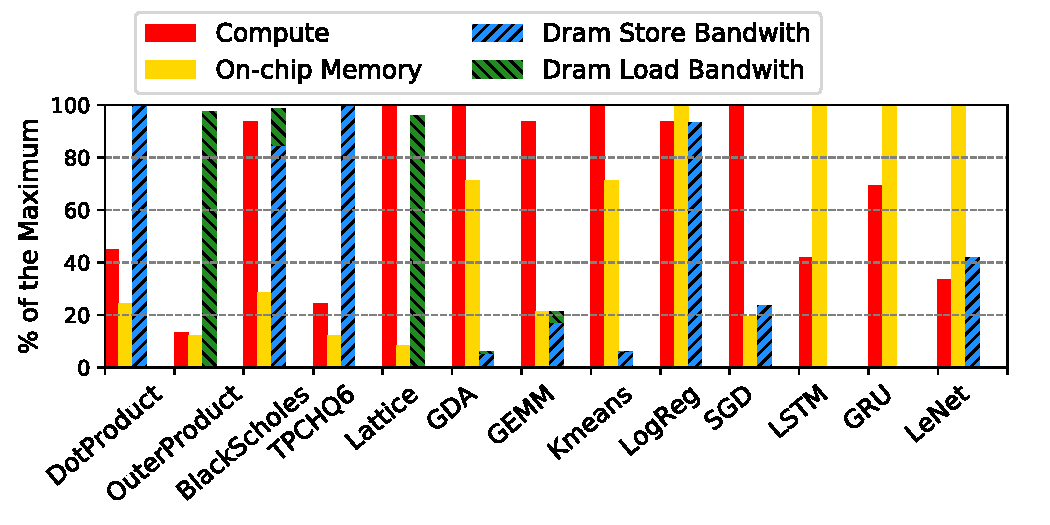
\includegraphics[width=0.8\columnwidth]{network/figs/util_bw2.pdf}
\caption[Resource and bandwidth utilization]{
  Physical resource and bandwidth utilization for various applications.}\label{fig:util_bw}
\centering
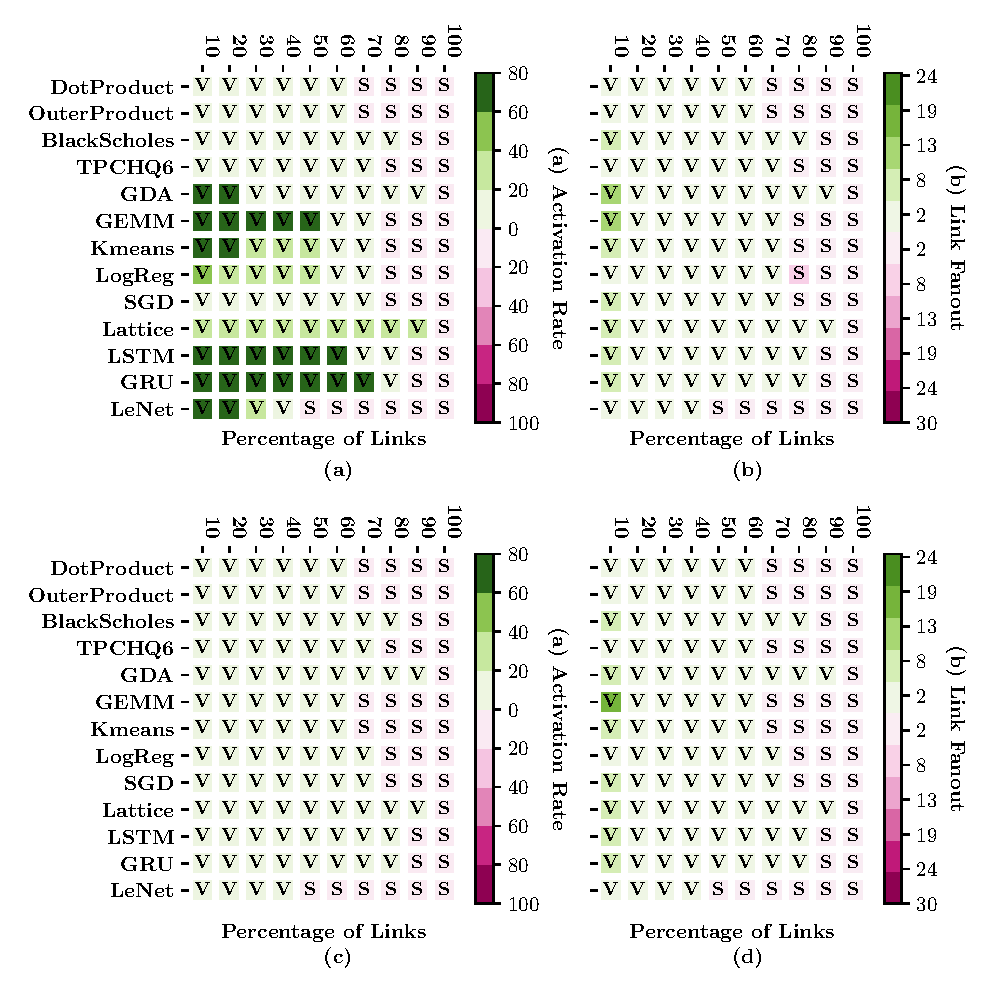
\includegraphics[width=0.8\columnwidth]{network/figs/link7.pdf}
  \caption[Application communication patterns]{Application communication patterns on pipelined (a,b) and scheduled (c,d) RDA architectures.
  (a) and (c) show the activation rate distribution of logical links at runtime. 
  Links sorted by granularity, then rate; darker boxes indicate higher rates.
  The split between green and pink shows the ratio of logical vector to scalar links. (b) and (d) show the distribution of broadcast link fanouts.
 }\label{fig:link}
\end{figure}

\begin{table*}
\centering
  \footnotesize
  \begin{tabular*}{6.25in}{p{0.75in} p{3in} p{2.5in}}
    \bottomrule
    \textbf{Benchmark} & \textbf{Description} & \textbf{Data Size} \\ \midrule
    DotProduct & Inner product & $1048576$ \\ \midrule
    OuterProduct & Outer product &$1024$ \\ \midrule
    BlackScholes & Option pricing &$1048576$ \\ \midrule
    TPCHQ6 & TPC-H query 6 &$1048576$ \\ \midrule
    Lattice & Lattice regression~\cite{garcia2009lattice} &$1048576$\\ \midrule
    GDA & Gaussian discriminant analysis &$127\times1024$ \\ \midrule
    GEMM & General matrix multiply &$256\times256\times256$ \\ \midrule
    Kmeans & K-means clustering &k=64, dim=64, n=8192, iter=2 \\ \midrule
    LogReg & Logistic regression &$8192\times128$, iter=4\\ \midrule
    SGD & Stochastic gradient descent for a single layer neural network &$16384\times64$, epoch=10 \\ \midrule
    LSTM & Long short term memory recurrent neural network &1 layer, 1024 hidden units, 10 time steps \\ \midrule
    GRU & Gated recurrent unit recurrent neural network &1 layer, 1024 hidden units, 10 time steps \\ \midrule
    LeNet & Convolutional neural network for character recognition& 1 image\\ \midrule
  \end{tabular*}
  \caption{Benchmark summary}
  \label{tab:benchmark}
\end{table*}

To study the communication patterns, 
we select a mix of applications from domains where hardware accelerators have shown promising performance and energy-efficiency benefits, such as linear algebra, databases, and machine learning.
Table~\ref{tab:benchmark} lists the applications and their data size.
Figure~\ref{fig:util_bw} shows, for each design, which resource limits performance: compute, on-chip memory, or DRAM bandwidth. 
DotProduct, TPCHQ6, OuterProduct, and BlackScholes are DRAM bandwidth-bound applications. 
These applications use few on-chip resources to achieve maximum performance, resulting in minimal communication.
Lattice (a fast inference model for low-dimensional regression~\cite{garcia2009lattice}), GDA, Kmeans, SGD, and LogReg are compute-intensive applications; for these, maximum performance requires using as much parallelization as possible. 
Finally, LSTM, GRU, and LeNet are applications that are limited by on-chip memory bandwidth or capacity. 
For compute- and memory-intensive applications, high utilization translates to a large interconnection network bandwidth requirement to sustain application throughput. 

Figure~\ref{fig:link}(a,b) shows the communication pattern of applications
characterized on the pipelined RDA architecture, including the variation in communication granularity. 
Compute and on-chip memory-bound applications show a significant amount of high-bandwidth communication (links with almost 100\% activity). 
A few of these high-bandwidth links also exhibit a high broadcast fanout. 
Therefore, a network architecture must provide sufficient bandwidth and efficient broadcasts to sustain program throughput.
On the contrary, time-scheduled architectures, shown in Figure~\ref{fig:link}(c,d), exhibit
lower bandwidth requirements due to the lower throughput of individual compute PUs. 
Even applications limited by on-chip resources have less than a 30\% firing rate on the busiest logical links; this reveals an opportunity for link sharing without sacrificing performance.

\begin{figure}
\centering
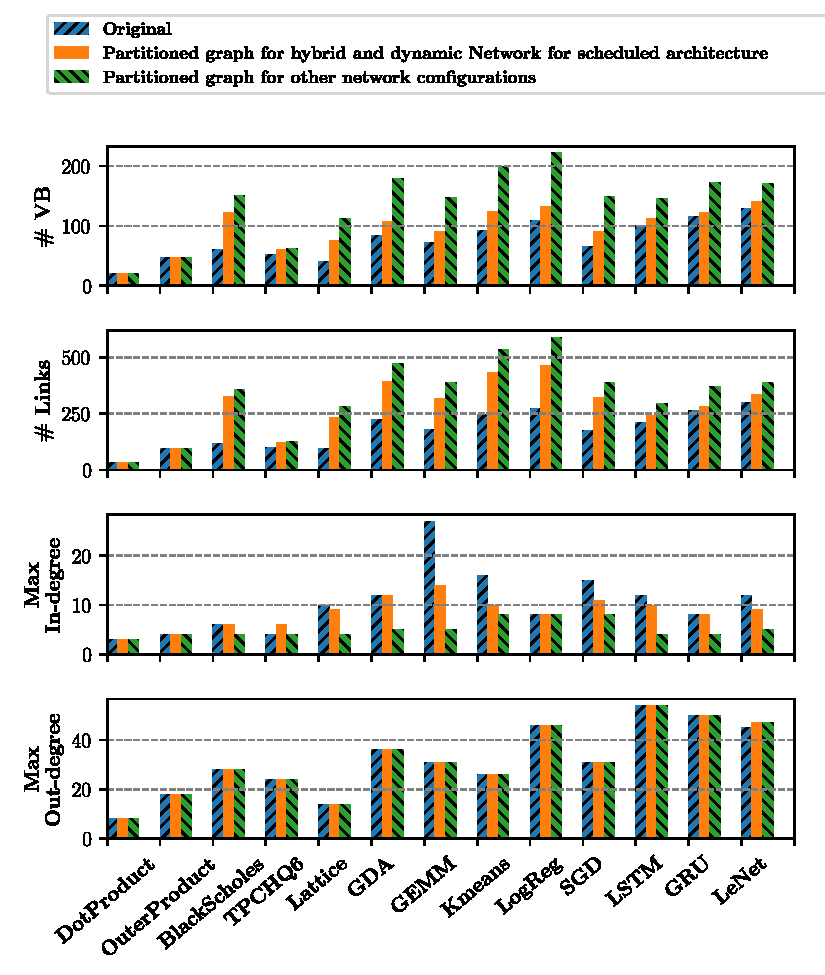
\includegraphics[width=0.9\columnwidth]{network/figs/graph.pdf}
\caption{Characteristics of program graphs.}\label{fig:graph}
\end{figure}

Figure~\ref{fig:graph} shows statistics describing the VU dataflow graph (VGDFG) before and after
the partitioning described in \Cref{sec:resalloc}. 
The blue bars show the number of VUs, number of logical links, and maximum VU input/output degrees in the original parallelized program; the yellow and green bars show the same statistics after partitioning. 
Fewer VUs are partitioned for hybrid networks and dynamic networks with the time-scheduled
architecture.
When a VU in a pipelined RDA consumes too many inputs or produces too many \emph{distinct} outputs,
\name partitions it to reduce its degree and meet the input/output bandwidth constraints of a purely static network. 
For dynamic and hybrid networks, partitioning is not strictly necessary, but it improves performance
by decreasing congestion at the network ejection port associated with a PU.
We do not partition broadcasts with high output degrees because they are handled natively within the network. 
Finally, the output degree does not change with partitioning because most outputs with a large degree are from broadcast links.

\subsection{Design Space for Network Architectures} \label{sec:networkds}

We start with several statically allocated network designs, where each SIMD pipeline connects to several switches, and vary flow control strategies and network bisection bandwidth.
In these designs, each switch output connects to exactly one switch input for the duration of the program.
We then explore a dynamic network, which sends program data as packets through an NoC.
The NoC uses a table-based routing scheme at each router to allow for arbitrary routes and tree-based broadcast routing.
Finally, we explore the benefits of specialization by evaluating design points that combine several of these networks to leverage the best features of each.

\subsubsection{Static networks}
We explore static network design points along three axes. 
First, we study the impact of flow-control schemes in static switches. 
In credit-based flow control~\cite{wang2013avoiding}, the source and destination PUs coordinate to ensure that the destination buffer does not overflow.
For this design point, switches only have a single register at each input, and there is no backpressure between switches.
The alternate design point uses a skid-buffered queue with two entries at each switch; using two entries enables per-hop backpressure and accounts for a one-cycle delay in stalling the upstream switch.
At full throughput, the receiver will consume data as it is sent and no queue will ever fill up.

The second axis studied is the bandwidth, and therefore routability, of the static network. 
We vary the number of connections between switches in each direction, which trades off area and energy for bandwidth.
Finally, we explore specializing static links: using a separate scalar network to improve routability at a low cost.

\subsubsection{Dynamic networks}
Our primary alternate design is a dynamic NoC using per-hop virtual channel flow control. 
Routing and Virtual Channel (VC) assignment are table-based: the compiler performs static routing and VC allocation, 
and results are loaded as a part of the routers' configurations at runtime.
The router has a separable, input-first VC and switch allocator with a single iteration and speculative switch allocation~\cite{dallytowles}.
Input buffers are sized just large enough (3 entries) to avoid credit stalls at full throughput.
Broadcasts are handled in the network with duplication occurring at the last router possible to minimize energy and congestion.
To respect the switch allocator's constraints, each router sends broadcasts to output ports sequentially and in a fixed order.
This is because the switch allocator can only grant one output port per input port in every cycle, and the RTL router's allocator does not have sufficient timing slack to add additional functionality.
We also explore different flit widths on the dynamic network, with a smaller bus taking multiple cycles to transmit a packet.

Because RDA networks are streaming---each PU pushes the result to the next PU(s) without explicit request---the network cannot handle routing schemes that may drop packets; otherwise, application data would be lost.
Because packet ordering corresponds directly to control flow, it is also imperative that all packets arrive in the order they were sent; this further eliminates adaptive or oblivious routing from consideration.
We limit our study of dynamic networks to statically placed and routed source routing due to these architectural constraints.
PUs propagate backpressure signals from their outputs to their inputs, so they must be considered as part of the network graph for deadlock purposes~\cite{hansson2007avoiding}.
Furthermore, each PU has fixed-size input buffers; these are far too small to perform high-throughput, end-to-end credit-based flow control in the dynamic network for the entire program \cite{wang2013avoiding}.
Practically, this means that no two logical paths may be allowed to conflict at \emph{any} point in the network; to meet this guarantee, VC allocation is performed to ensure that all logical paths traversing the same physical link are placed into separate buffers.

\subsubsection{Hybrid networks}
Finally, we explore hybrids between static and dynamic networks that run each network in parallel. 
During static place and route, the highest-bandwidth logical links from the program graph are mapped onto the static network; once the static network is full, further links are mapped to the dynamic network.
By using compiler knowledge to identify the relative importance of links---the link fanout and activation factor---hybrid networks can sustain the throughput requirement of most high-activation links while using the dynamic network for low-activation links.

\subsection{Performance, Area, and Energy Modeling} \label{sec:net_char}

Next section gives a quantitative analysis of the performance, area, and energy trade-offs involved 
in choosing a RDA network, using benchmarks showing in \Cref{tab:benchmark}.
This section outlines our methodology on how we capture the network performance, area, and energy in our evaluations.
\Cref{tab:notation} gives our notation for various network parameters discussed
in~\Cref{sec:networkds}.

\begin{table}
\footnotesize
  \centering
\begin{tabular*}{0.65\textwidth}{c l}
  \bottomrule
  \textbf{Notation} & \textbf{Description} \\\midrule
  $[$S,H,D$]$ & Static, hybrid, and dynamic network \\\midrule
  x<\#> & Static bandwidth on vector network (\#links between switches) \\\midrule
  %$s\#$ & Number of links between switches on static scalar network \\\midrule
  f<\#> & Flit width of a router or vector width of a switch \\\midrule
  v<\#> & Number of VC in router \\\midrule
  b<\#> & Number of buffers per VC in router \\\midrule
  $[$db,cd$]$ & Buffered vs. credit-based flow control in switch \\\midrule
  %$[Scheduled, Pipelined]$ & Time scheduled vs deep pipelined accelerator architectures \\\midrule
\end{tabular*}
\caption{Network design parameter summary.}
\label{tab:notation}
\end{table}

\subsubsection{Simulation}
We use a cycle-accurate simulator to model the pipeline and scheduling delay for the two types of architectures,
 integrated with DRAMSim \cite{dramsim} to model DRAM access latency. For static networks, we model
a distance-based delay for both credit-based and per-hop flow control. 
For dynamic networks, we integrate
our simulator with Booksim \cite{jiang2013detailed}, adding support for arbitrary source routing using look-up tables. 
Finally, to support efficient multi-casting in the dynamic network, we modify Booksim to duplicate broadcast packets at the router where their paths diverge.
At the divergence point, the router sends the same flit to multiple output ports over multiple cycles.
We assume each packet carries a unique ID that is used to look up the output port and next VC in a statically generated routing table, and that the ID is roughly the same size as an address.
When the packet size is greater than the flit size, the transmission of a single packet takes multiple cycles.

\subsubsection{Area and power}
To efficiently evaluate large networks, we start by characterizing the area and power consumption of individual routers and switches
used in various network configurations. 
The total area and energy are then aggregated over all switches and routers in a particular network.
We use router RTL from the Stanford open-source NoC router \cite{becker2012efficient} and our own parameterized switch implementation.
We synthesize using Synopsys Design Compiler with a \SI{28}{nm} technology library and clock-gating enabled, meeting timing at a 1 GHz clock frequency.
Finally, we use Synopsys PrimeTime to back-annotate RTL signal activity to the post-synthesis switch and router designs to estimate gate-level power.

We found that power consumption can be broken into two types: 
inactive power consumed when switches and routers are at zero-load ($P_{\text{inactive}}$, which includes both dynamic and static power),
and active power. The active power, as shown in Section~\ref{sec:net_char}, is proportional to the amount of
data transmitted. 
Because power scales linearly with the amount of data movement, we model the marginal energy to transmit a single flit of data (flit energy, $E_{\text{flit}}$) by dividing active energy by the number flits transmitted in the testbench:
\begin{equation}
  E_{\text{flit}} = \frac{\left(P-P_{\text{inactive}}\right) T_{\text{testbench}}}{\#\text{flit}} 
\end{equation}
While simulating an end-to-end application, we track the number of flits transmitted at each switch and router in the network, as well as the number of switches and routers allocated by place and route. 
We assume unallocated switches and routers are perfectly power-gated and do not consume energy.
The total network energy for an application on a given network ($E_{\text{net}}$) can be computed as:
\begin{equation}
  E_{\text{net}} = \sum_{\text{allocated}} P_{\text{inactive}} T_{\text{sim}}
  + E_{\text{flit}}  \#\text{flit},
\end{equation}
where $P_{\text{inactive}},$ $E_{\text{flit}},$ and $\#\text{flit}$ are tabulated separately for each network resource.

\begin{figure}
\centering
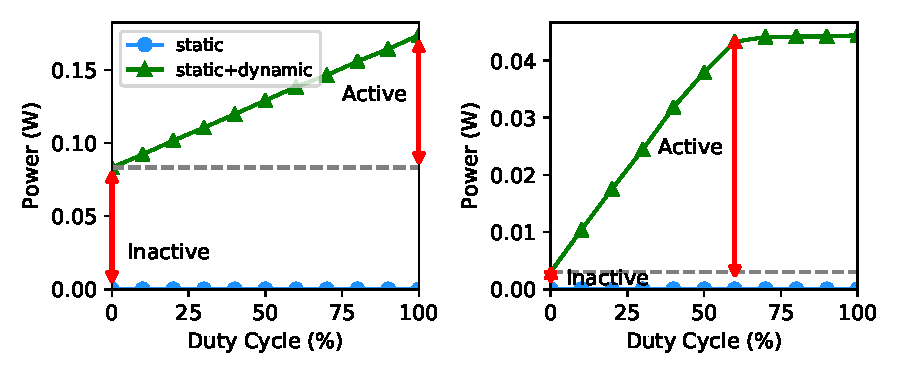
\includegraphics[width=0.8\columnwidth]{network/figs/sweep.pdf}
  \caption{Switch and router power with varying duty cycle.}\label{fig:sweep}
\end{figure}


Figure~\ref{fig:sweep} shows that switch and router power scale linearly with the rate of data transmission, but that there is non-zero power at zero-load. 
For simulation, the duty cycle refers to the amount of offered traffic, not accepted traffic.
Because our router uses a crossbar without speedup \cite{dallytowles}, the testbench saturates the router at 60\% duty cycle when providing uniform random traffic. 
Nonetheless, router power still scales linearly with accepted traffic.

A sweep of different switch and router parameters is shown in Figure~\ref{fig:char}. Subplots (d,e,f) show the energy necessary to transmit a single bit through a switch or router.
Subplot (a) shows the roughly quadratic scaling of switch area with the number of links between adjacent switches.
Vector switches scale worse with increasing bandwidth than scalar switches, mostly due to increased crossbar wire load. 
At the same granularity, a router consumes more energy a switch to transmit a single bit of data, even though the overall router consumes less power (as shown in Figure~\ref{fig:sweep}); 
this is because the switch has a higher throughput than the router.
The vector router has lower per-bit energy relative to the scalar router because it can amortize the cost of allocation logic, whereas the vector switch has higher per-bit energy relative to the scalar switch due to increased capacitance in the large crossbar. 
Increasing the number of VCs or buffer depth per VC also significantly increases router area and energy, but reducing the router flit width can significantly reduce the router area. 

\begin{figure}
\centering
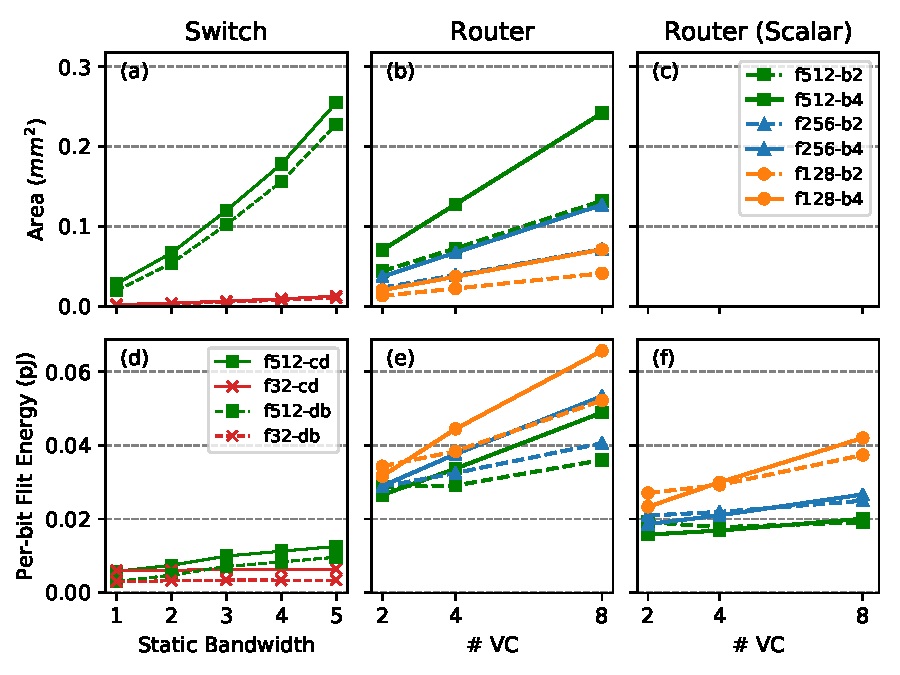
\includegraphics[width=0.8\columnwidth]{network/figs/char.pdf}
  \caption{Area and per-bit energy for (a,d) switches and (b,c,f) routers. 
  The router only has a vector granularity and can be partially clock-gated when sending scalar packets.
  Subplots (f) show the energy of the vector router when used for scalar values (32-bit).}\label{fig:char}
\end{figure}

Overall, these results show that scaling static bandwidth is cheaper than scaling dynamic bandwidth, and a dynamic network with small routers can be used to improve link sharing for low bandwidth communication.  
We also see that a specialized scalar network, built with switches, adds a negligible area compared to and is more energy-efficient than the vector network. 
Therefore, we use a static scalar network with a bandwidth of 4 for the remainder of our evaluation, except when evaluating the pure dynamic network.
The dynamic network is also optimized for the rare instances when the static scalar network is insufficient. 
When routers transmit scalar data, the high bits of data buffers are clock-gated, reducing energy as shown in (f).
Figure~\ref{fig:area} summarizes the area breakdown of all the network configurations that we evaluate.

\begin{figure}
\centering
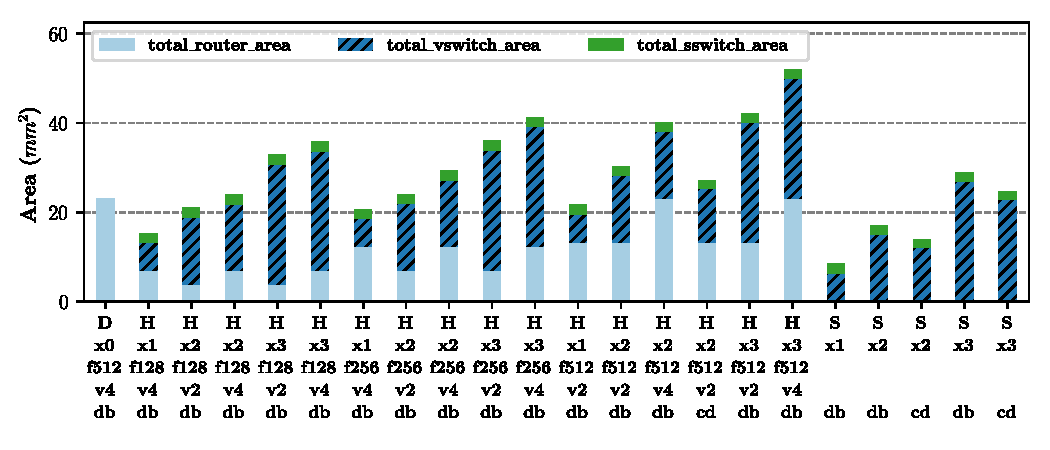
\includegraphics[width=1\columnwidth]{network/figs/area.pdf}
  \caption{Area breakdown for all network configurations.}\label{fig:area}
\end{figure}

\subsection{Network Architecture Evaluation} \label{sec:net_dse}

We evaluate our network configurations in five dimensions: performance (perf), performance per network area (perf/area), performance per network
power (perf/watt), network area efficiency (1/area), and network power efficiency (1/power). 
Among these metrics, performance is the most important: networks only consume a small fraction of the overall accelerator area and energy (roughly 10-20\%). 
Because the two key advantages of hardware accelerators are high throughput and low latency, 
we filter out a network design point if it introduces
more than 10\% performance overhead.
This is calculated by comparing to an ideal network with infinite bandwidth and zero latency.

For metrics that are calculated per application, such as performance, performance/watt, and power efficiency, we first normalize the metric with respect to the 
worst network configuration for that application. 
For each network configuration, we present a geometric mean normalized across all applications. 
For all of our experiments, except Section~\ref{sec:scale}, we use a network
size of $14\times14$ end-point PUs. All vector networks use a vectorization factor of 16 (\SI{512}{bit} messages).

\begin{figure}
\centering
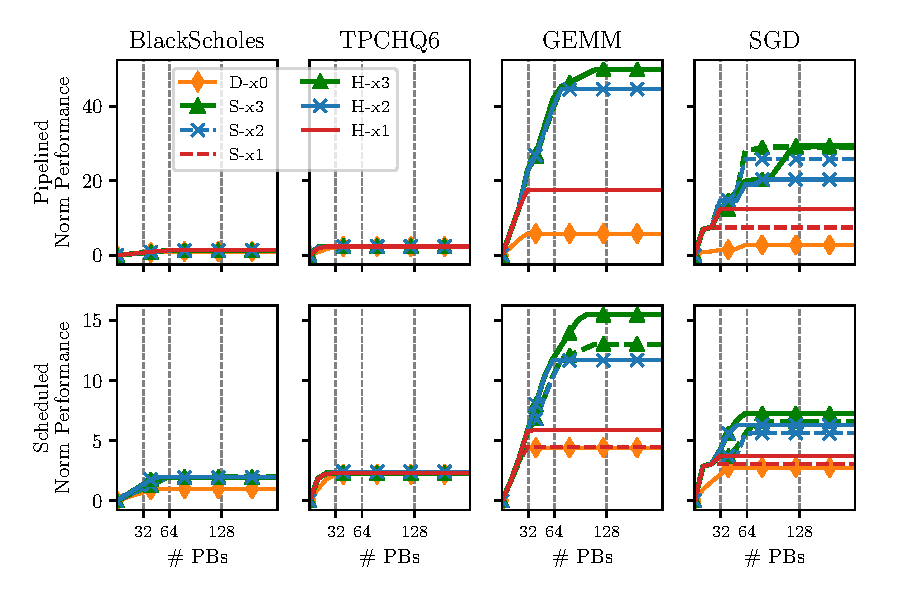
\includegraphics[width=0.8\columnwidth]{network/figs/scale.pdf}
\caption{Performance scaling with increased RDA grid size for different networks.}\label{fig:scale}
\end{figure}
\subsubsection{Bandwidth scaling with network size}\label{sec:scale}
Figure~\ref{fig:scale} shows how different networks allow several applications to scale to different numbers of PUs.
For IO-bound applications (BlackScholes and TPCHQ6), performance does not scale with additional compute and on-chip memory resources.
However, the performance of compute-bound applications (GEMM and SGD) improves with increased resources, but plateaus at a level that is determined by on-chip network bandwidth. 
This creates a trade-off in accelerator design between highly vectorized compute PUs with a small network---which would be underutilized for non-vectorized problems---and smaller compute PUs with limited performance due to network overhead. 
For more finely grained compute PUs, both more switches and more costly (higher-radix) switches must be employed to meet application requirements.

The scaling of time-scheduled accelerators (bottom row) is much less dramatic than that of deeply pipelined architectures (top row). 
Although communication between PUs in these architectures is less frequent, the scheduled architecture must use additional parallelization to match the throughput of the pipelined architecture; this translates to larger network sizes. 

For pipelined architectures, both hybrid and static networks provide similar scaling with the same static bandwidth:
the additional bandwidth from the dynamic network in hybrid networks does not provide additional scaling. 
This is mostly due to a bandwidth bottleneck between a PU and its router, which prevents the PU from requesting multiple elements per cycle.
Hybrid networks tend to provide better scaling for time-scheduled architectures; multiple streams can be time-multiplexed at each ejection port without losing performance.

\subsubsection{Bandwidth and flow control in switches}

\begin{figure}
  \centering
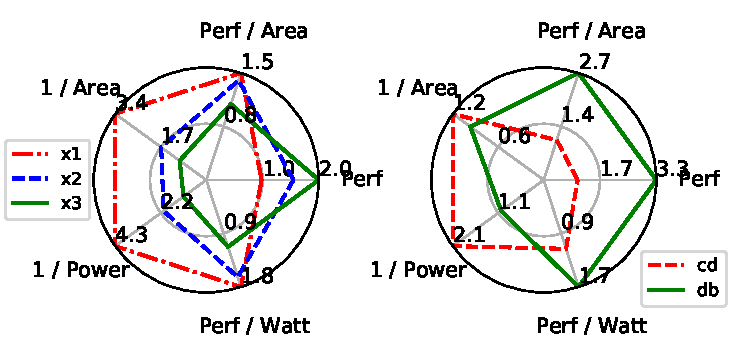
\includegraphics[width=0.7\textwidth]{network/figs/radar_switch.pdf}
  \caption{
    Impact of bandwidth and flow control strategies in switches.}\label{fig:radar_switch}
\end{figure}

In this section, we study the impact of static network bandwidth and flow control mechanisms (per-hop vs. end-to-end credit-based). 
On the left side of Figure~\ref{fig:radar_switch}, we show that increased static bandwidth results in a linear performance increase and a superlinear increase in area and power. 
As shown in Section~\ref{sec:scale}, any increase in accelerator size must be coupled with increased network bandwidth to effectively scale performance. 
This indicates that network overhead will increase with the size of an accelerator.

The right side of Figure~\ref{fig:radar_switch} shows that, although credit-based flow control reduces the amount of buffering in switches and decreases network area and energy, application performance is significantly impacted. 
This is the result of imbalanced data-flow pipelines in the program: when there are parallel long and short paths over the network, there must be sufficient buffer space on the short path equal to the product of throughput and the difference in latency. 
Because performance is our most important metric, credit-based flow control is not feasible, especially because the impact of bubbles increases with communication distance, and therefore network size.

\subsubsection{VC count and reduced flit width in routers}
\begin{figure}
  \centering
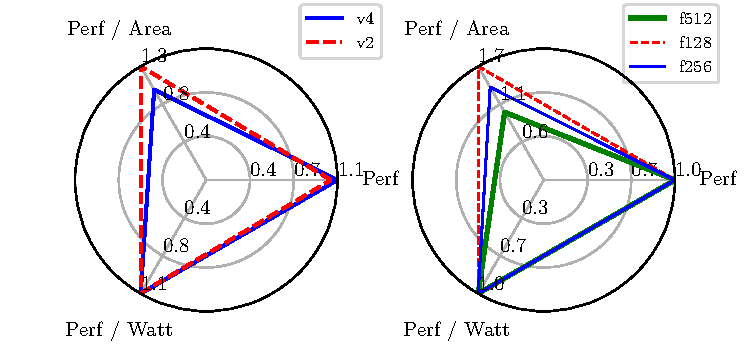
\includegraphics[width=0.7\textwidth]{network/figs/radar_router.pdf}
  \caption{Impact of VC count and flit widths in routers.}\label{fig:radar_router}
\end{figure}
In this experiment, we study the area-energy-performance trade-off between routers with different VC counts. As shown
in Section~\ref{sec:net_char}, using many VCs increases both network area and energy.
However, using too few VCs may force roundabout routing on the dynamic network or result in VC allocation failure when the network is heavily utilized.
Nonetheless, the left side of Figure~\ref{fig:radar_router} shows minimal performance improvement from using more VCs. 

Therefore, for each network design, we use a VC count equal to the maximum number of VCs required to map all applications to that network. 
Figure~\ref{fig:vc} shows that the best hybrid network configurations with 2x and 3x static bandwidth require at most 2 VCs, whereas the pure dynamic network requires 4 VCs to map all applications.
Because dynamic network communication is infrequent, hybrid networks with fewer VCs provide both better energy and area efficiency than networks with more VCs, even though this constrains routing on the dynamic network.

\begin{figure}
\centering
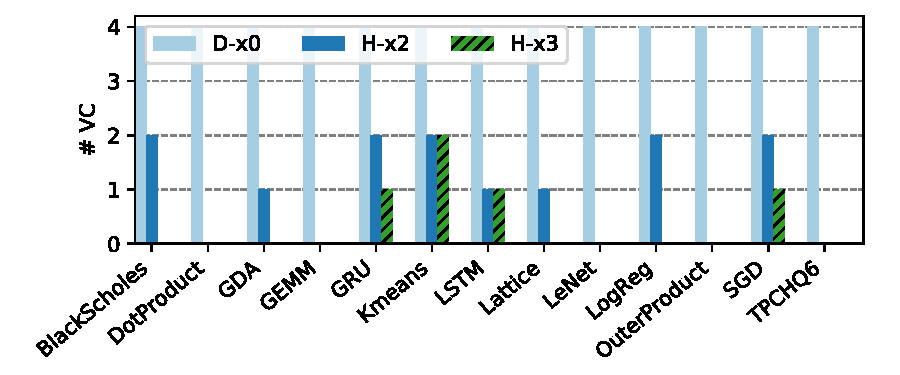
\includegraphics[width=0.75\textwidth]{network/figs/vc.pdf}
  \caption{Number of VCs required for dynamic and hybrid networks. (No VCs indicates that all traffic is mapped to the static network.)}\label{fig:vc}
\end{figure}

We also explore the effects of reducing dynamic network bandwidth by using smaller routers;
as shown in Section~\ref{sec:net_char}, routers with smaller flits have a much smaller area.
Ideally, we could scale static network bandwidth while using a low-bandwidth router to provide an escape path and reduce overall area and energy overhead. 
The right side of Figure~\ref{fig:radar_router} shows that, for a hybrid network, reducing flit width improves area efficiency with minimal performance loss. 

\subsubsection{Static vs. hybrid vs. dynamic networks}

\begin{figure*}
\centering
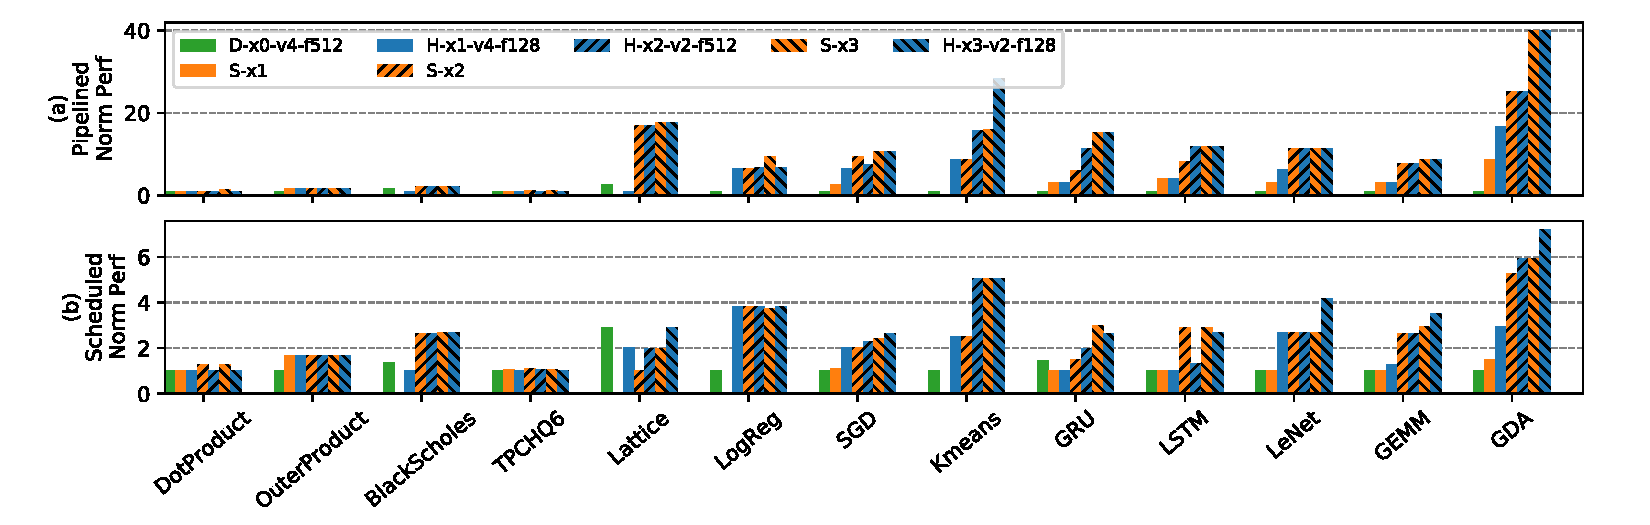
\includegraphics[width=1\linewidth]{network/figs/perf.pdf}
  \caption{Normalized performance for different network configurations.}\label{fig:perf}
\end{figure*}

Figure~\ref{fig:perf} shows the normalized performance for each application running on several network configurations.
For some applications, the bar for S-x1 is missing; this indicates that place and route failed for all unrolling factors.
For DRAM-bound applications, the performance variation between different networks is trivial because only a small fraction of the network is being used. 
In a few cases (Kmeans and GDA), hybrid networks provide better performance due to slightly increased bandwidth.
For compute-bound applications, performance primarily correlates with network bandwidth because more bandwidth permits a higher parallelization factor. 

\begin{figure}
\centering
  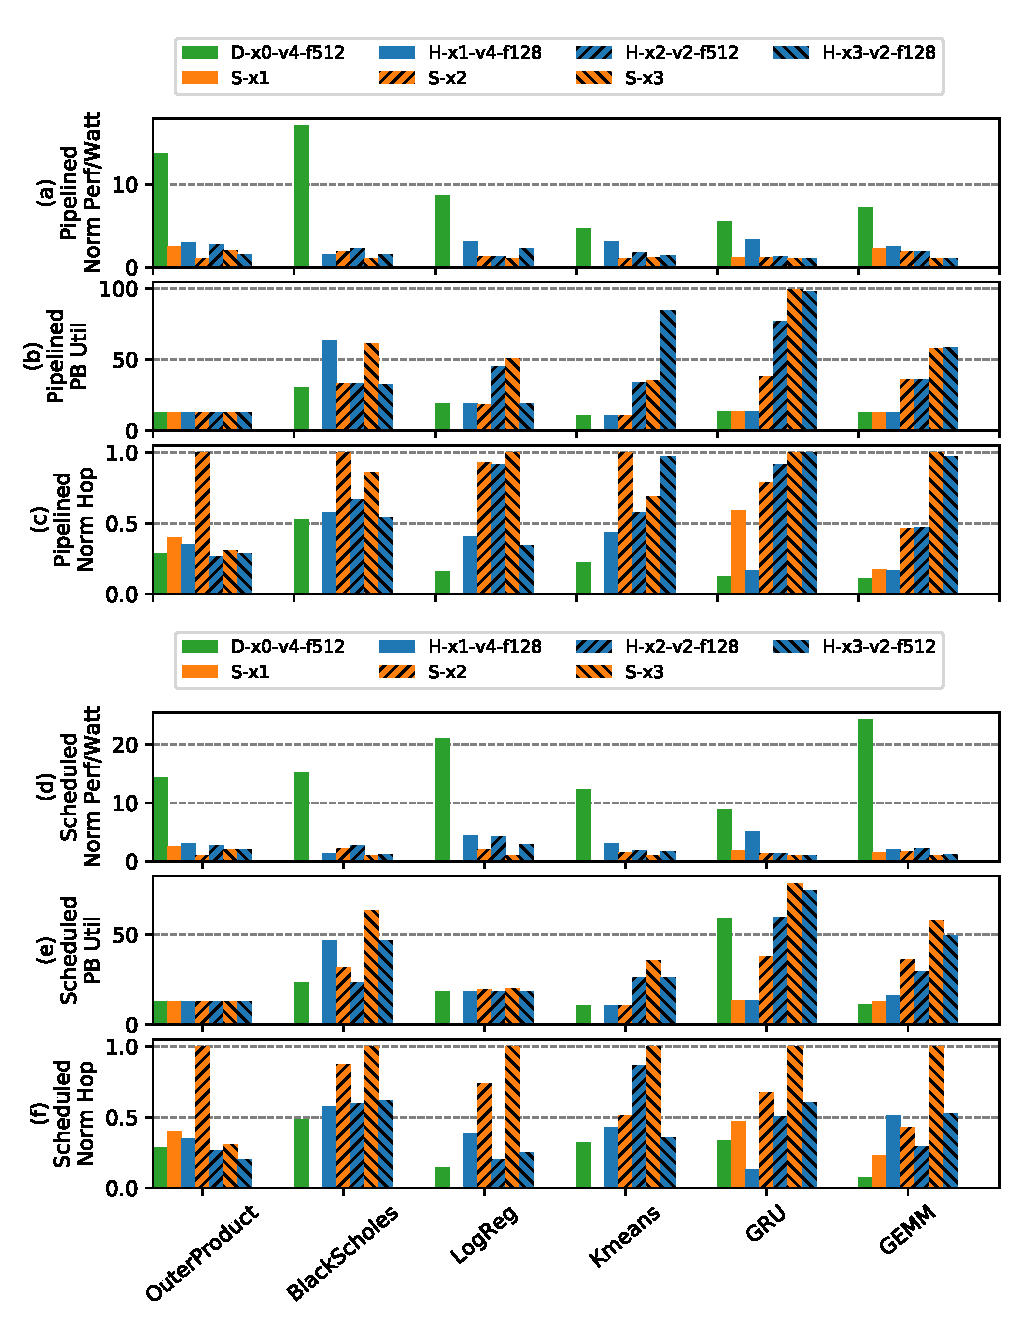
\includegraphics[width=0.9\textwidth]{network/figs/energy.pdf} 
\caption{(a,d): Normalized performance/watt. (b,e): Percentage of compute and memory PUs utilized for each network configuration. 
  (c,f): Total data movement (hop count).}
\label{fig:energy}
\end{figure}

The highest bandwidth static network uses the most PUs, as shown in Figures~\ref{fig:energy}(b,e), because it permits more parallelization. 
It also has more data movement, as shown in (c,f), because PUs can be distributed farther apart. 
Due to bandwidth limitations, low-bandwidth networks perform best with small unrolling factors---they are unable to support the bisection bandwidth of larger program graphs.
This is evident in Figures~\ref{fig:energy}(b,e), where networks D-x0-v4-f512 and S-x2 have small PU utilizations.

With the same static bandwidth, most hybrid networks have better energy efficiency than the corresponding pure static networks, even though routers take more energy than switches to transmit the same amount of data.
This is a result of allowing a small amount of traffic to escape onto the dynamic network: with the dynamic network as a safety net, static PaR tends to converge to better placements with less overall communication.
This can be seen in Figures~\ref{fig:energy}(c,f), where most static networks have larger hop counts than the corresponding hybrid network; hop count is the sum of all runtime link traversals, normalized per-application to the network configuration with the most hops.
Subplots (e,f) show that more PUs are utilized with static networks than hybrid networks.
This is because the compiler imposes less stringent IO constraints on PUs when partitioning for the hybrid network (as explained in Section~\ref{sec:partition}), which results in fewer PUs, less data movement, and greater energy efficiency for hybrid networks.

\begin{figure}
  \centering
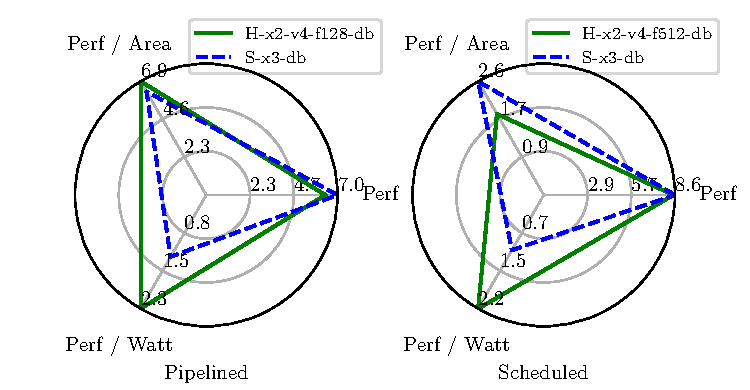
\includegraphics[width=0.7\textwidth]{network/figs/radar_best.pdf}
  \caption{Geometric mean improvement for the best network configurations, relative to the worst configuration.}\label{fig:radar_best}
\end{figure}
\begin{figure*}
\centering
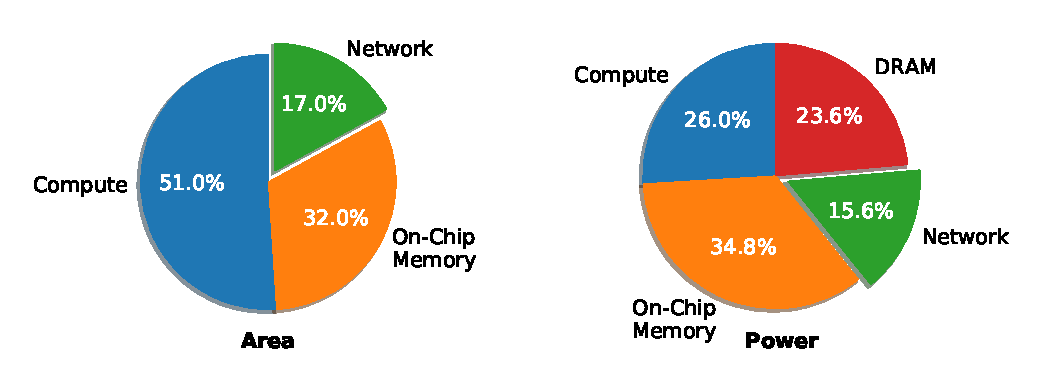
\includegraphics[width=0.8\textwidth]{figs/pie.pdf}
\caption[Area and power breakdown of Plasticine]{
  Area and power breakdown of Plasticine using a static-dynamic hybrid network.
}
\label{fig:breakdown}
\end{figure*}

In Figure~\ref{fig:radar_best}, we summarize the best perf/watt and perf/area (among network configurations with <10\% performance overhead) for pipelined and scheduled RDA architectures. 
Pure dynamic networks are not shown because they perform poorly due to insufficient bandwidth.
On the pipelined RDA, the best hybrid network provides a 6.4x performance increase, 2.3x better energy efficiency, and a 6.9x perf/area increase over the worst network configuration. 
The best static network provides 7x better performance, 1.2x better energy efficiency, and 6.3x better perf/area. 
The hybrid network gives the best perf/area and perf/watt, with a small degradation in performance when compared to the static network. 
On the time-scheduled RDA, both static and hybrid networks have an 8.6x performance improvement. 
The hybrid network gives a higher perf/watt improvement at 2.2x, whereas the static network gives a higher perf/area improvement at 2.6x.
Overall, the hybrid networks deliver better energy efficiency with shorter routing distances by allowing an escape path on the dynamic network.

\section{Plasticine Specialization for RNN Serving} \label{sec:rnn_arch}
To show efficient execution of the loop and parallel pattern constructs,
  we map our implementation onto a spatial architecture, Plasticine.
\textbf{Foreach} at Line $17, 19$ and \textbf{Reduce} at Line $22, 23$
  are mapped to PCUs on Plasticine.
When the application size is small,
  these constructs are executed using pipelined SIMD lanes within a single PCU.
When the application size is large,
  multiple PCUs can be used to parallelize and pipeline the dot
  product across PCUs. Element-wise operations can be executed in a deep pipeline
  formed by chaining multiple PCUs.

To fit an RNN's weights on-chip,
  we execute our application with low-precision arithmetics.
In this section,
  we propose the necessary micro-architectural changes to
  support low-precision arithmetics on Plasticine.
We also discuss architectural parameter selection for Plasticine
  to serve RNN applications efficiently.

\subsection{Mixed-Precision Support}
\label{sec:arch:varprec}
Previous works \cite{fowers2018configurable, jouppi2017datacenter}
  have shown that low-precision inference can deliver promising performance
  improvements without sacrificing accuracy.
In the context of reconfigurable architectures such as FPGAs,
  low-precision inference not only increases compute density,
  but also reduces required on-chip capacity for
  storing weights and intermediate data.

To support low-precision arithmetics without sacrificing coarse-grained reconfigurability,
we introduce two low-precision struct types in Spatial: a tuple of 4 8-bit and 2 16-bit floating-point 
numbers, \texttt{4-float8} and \texttt{2-float16} respectively.
Both types packs multiple low-precision values into a single precision storage.
We support only 8 and 16-bit precisions, which are commonly seen in deep learning inference hardwares.
Users can only access values that are 32-bit aligned.
This constraint guarantees that the microarchitectual change is only local to the PCU.
Banking and DRAM access granularity remains intact from the original design.

\begin{figure}
  \centering
  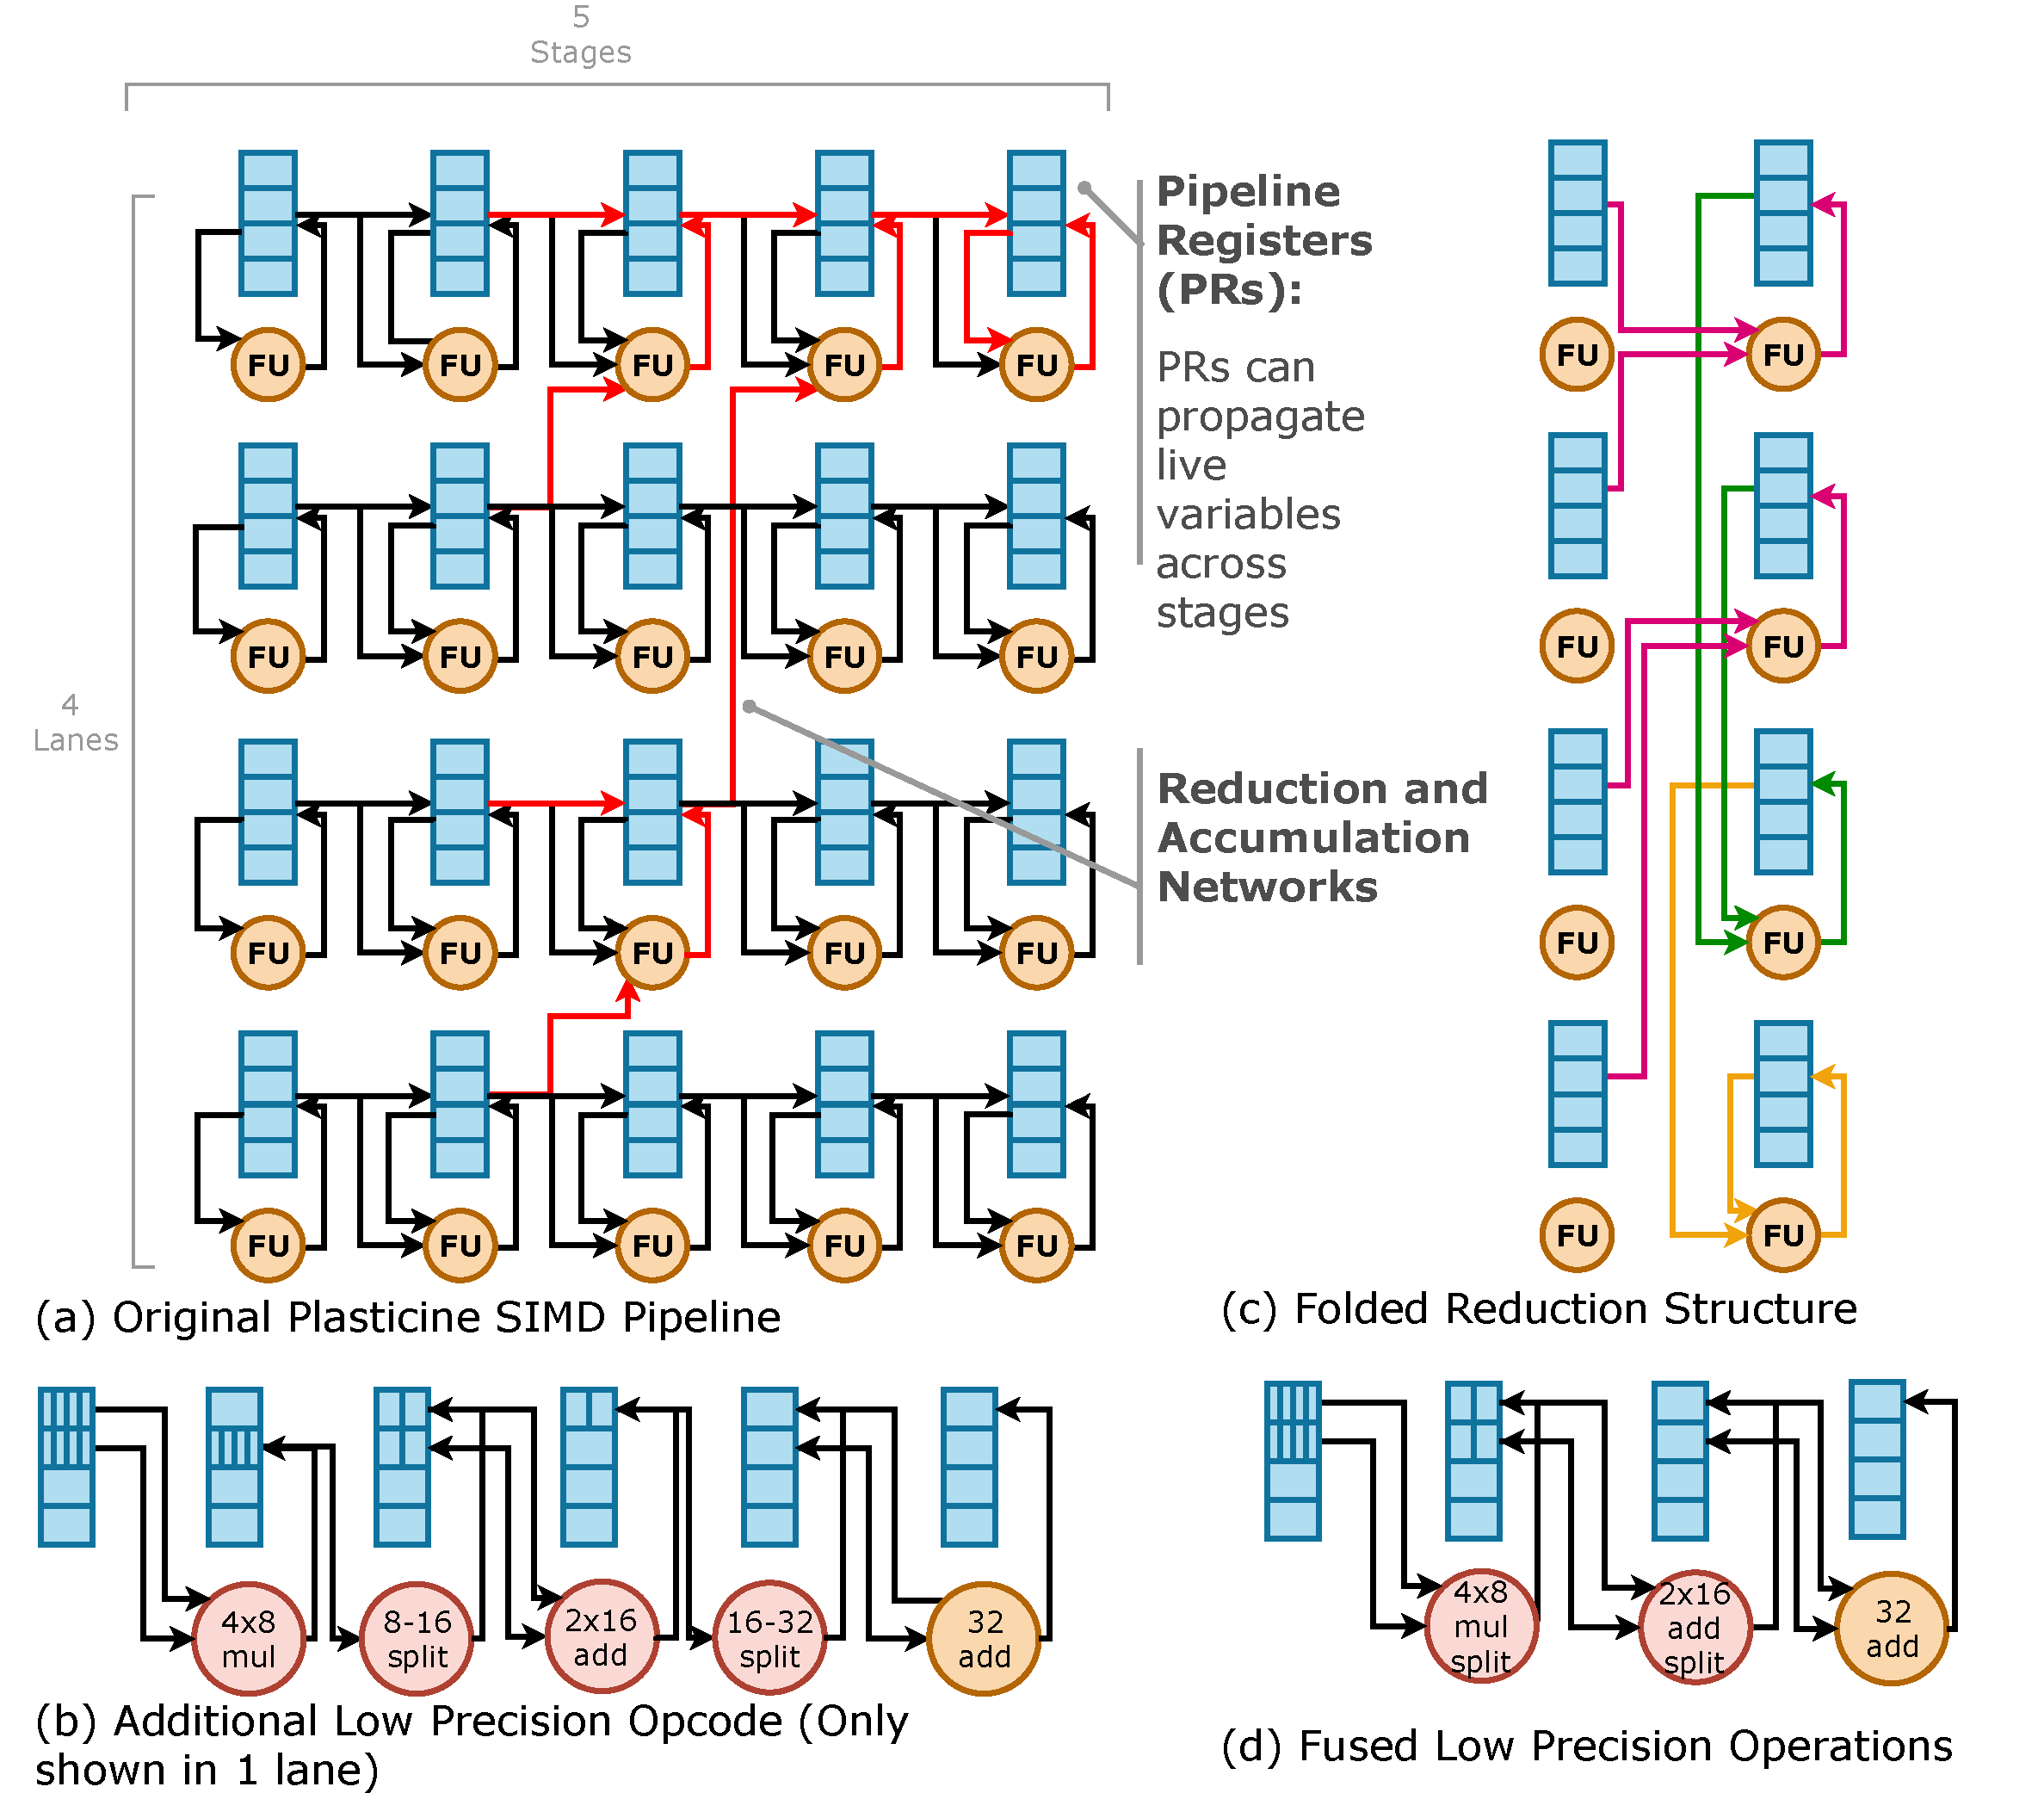
\includegraphics[width=1\columnwidth]{figs/lowprec.pdf}
  \caption{Plasticine PCU SIMD pipeline and low-precision support.
  Red circles are the new operations. Yellow circles are the original opertaions in Plasticine.
  In (d) the first stage is fused $1^{st}, 2^{nd}$ stages, and the second stage is fused
  $3^{nd}$, $4^{th}$ stages of (b).
   }
  \label{fig:lowprec}
  \vspace*{-0.3in}
\end{figure}
Figure \ref{fig:lowprec} (a) shows the original SIMD pipeline in a Plasticine PCU.
Each FU supports both floating-point and fix-point operations.
When mapping applications on Plasticine,
  the inner most loop body is vectorized across the lanes of the
SIMD pipeline, and different operations of the loop body are mapped to different stages.
Each pipeline stage contains a few pipeline registers (PRs)
  that allow propagation of live variables across stages.
%The PRs are accessible as both inputs and outputs of the FU.
%An FU can also read previous stage's PRs
%as its input value.
Special cross-lane connections as shown in red in Figure \ref{fig:lowprec} enable reduction operations.
To support 8-bit element-wise multiplication and 16-bit reduction, we add 4 opcodes to the FU, shown in
Figure \ref{fig:lowprec} (b).
The $1^{st}$ and $3^{rd}$ stages are element-wise, low-precision operations
  that multiply and add 4 8-bit and 2 16-bit values, respectively.
The $2^{nd}$ and $4^{th}$ stages rearrange low-precision values into two registers,
  and then pad them to higher precisions.
The $5^{th}$ stage reduces the two 32-bit value to a single 32-bit value using the existing add operation. 
From here, we can use the original
reduction network shown in Figure \ref{fig:lowprec} (a) to complete the remaining reduction and accumulates
in 32-bit connection.

With 4 lanes and 5 stages,
  a PCU first reads 16 8-bit values,
  performs 8-bit multiplication followed by rearrangement and padding,
  and then produce 16 16-bit values after the second stage.
The intermediate values are stored in 2 PRs per lane.
Next, 16 16-bit values are reduced to 8 16-bit values
  and then rearranged to 8 32-bit value in 2 PRs per lane.
Then, the element-wise addition in 32-bit value
  reduces the two registers in each line into 4 32-bit values.
These values are fed through the
  reduction network that completes the remaining
  reduction and accumulation in two plus one stages.

In a more aggressive specialization,
  we can fuse the multiply and rearange into the same stage.
We also fuse the first low-precision reduction with the next rearange as shown in Figure \ref{fig:lowprec} (d).
In this way, we can perform the entire low-precision map-reduce in 2 stages
  in addition to the original full precision reduction.
In order to maximize hardware reuse,
  we assume that it is possible to construct a full precision FU
  using low-precision FUs.
In addition, we observe that the original reduction network in the SIMD lanes
  could lead to low FU utilization.
To improve FU utilization, we fold the entire tree structure in a single stage.
Figure \ref{fig:lowprec} (c) shows the folded reduction accumulation structure.
Specifically, latter reductions in the tree are mapped to earlier stages in the pipeline.
In this setup, the entire reduction plus accumulation
  is still fully pipelined in $\log_2(\#_{LANE})+1$ cycles
  with no structural hazard.
With fused reduced-precision multiplication and reduction, and folded reduction tree,
  a PCU is able to perform all map-reduce that accumulates $4 \#_{LANE}$
  8-bit values using 4 stages.
All the operations are completed in $2+\log_2(\#_{LANE})+1$ cycles.

\subsection{Sizing Plasticine for RNN Serving}
Evaluating an RNN cell containing $N$ hidden units and $N$ input features
  requires $2N^2$ computations and $N^2+N$ memory reads.
With large $N$, the compute to memory ratio is 2:1.
The original Plasticine architecture uses a checkerboard layout
  with 1 to 1 ratio between PCU and PMU.
A PCU has 6 stages and 16 lanes, and a PMU has 16 banks.
This provides a 6:1 ratio between
  compute resource and on-chip memory read bandwidth.
As a result of this layout,
  on-chip memory read bandwidth becomes the bottleneck for accelerating RNN serving applications.
Given that RNNs cover a wide range of important applications,
  we select a Plasticine configuration tailored for RNN serving.
Specifically, we choose a 2 to 1 PMU-PCU ratio with 4 stages in each PCU.
Figure \ref{fig:arch} shows the layout of this Plasticine variant.
\begin{figure}
  \centering
  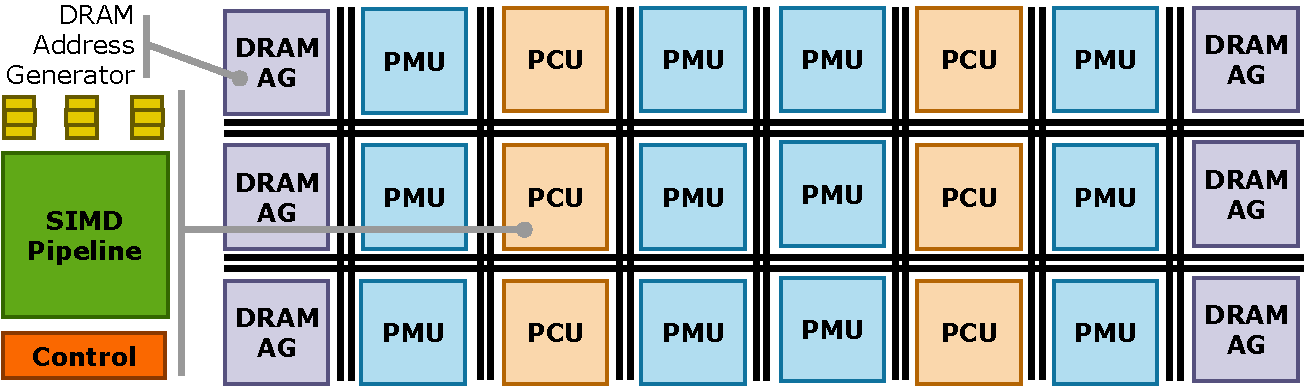
\includegraphics[width=\columnwidth]{figs/arch.pdf}
  \caption{Variant configuration of Plasticine for serving RNN.}
  \label{fig:arch}
  \vspace*{-0.2in}
\end{figure}

\section{Generic Banknig Support (Ready)} \label{sec:banking_arch}

To support Spatial's generic banking scheme for on-chip SRAM mentioned in \Cref{sec:memsplit}, 
we need to introduce a few microarchitectural changes to Plasticine's datapath.
As a background, the static banking analysis searches an address remapping scheme, which we refer as
banking scheme, that remaps the logical address space into partitions, such that addresses accessed
in parallel belongs to different partitions. 
Each partition corresponds to a physical memory bank that comes with an additional address port.
If the compiler can find a way to partition the data such that all parallel workers are sent to
different physical banks, the memory is guaranteed to feed all workers at full-throughput, which
scales performance with parallelism.
To search for the banking schemes, the compiler analyzes the access patterns of the memory.
An access pattern refers to groups of address expressions that can be queried concurrently.
For each access pattern, there can be multiple banking schemes that can sustain the access bandwidth.
However, not all schemes cost the same amount of resources; some are more expensive in logic, and
others are more expensive in memory.

The partitioning logic are two parametrizable equations for the bank address (BA) and the bank offset (BO),
both are functions of the original user-requested logical addresses.
BA is an expression that selects the partition for each request, and BO is the offset within the partition.
The banking analyzer searches the parameters in the equation and injects these computations to
memory accesses in the program. 
The first addition to Plasticine is the ability to compute independent BI and BO for each vector
lanes. 
We introduce vectorized address pipelines in PMUs, which was originally a scalar pipeline.

The generic banking scheme also requires a full crossbar datapath between all access lanes (workers) and
physical banks. To support this, we introduce the shuffle operator shown in \Cref{fig:memsplit}.
The shuffle operator takes three vectorized operands: a from address $\overrightarrow{FA}$, a to address
$\overrightarrow{TA}$, and a base $\overrightarrow{B}$.
The output $O$ equals to $B$ shuffled from the order specified in $\overrightarrow{FA}$ to the order in
$\overrightarrow{BA}$. 
Specifically,
\begin{align}
\forall i \in [1,|\overrightarrow{O}|],
O_i &= \begin{cases}
B_j, \text{if $\exists$ $TA_i = FA_j$}\\
0
\end{cases} \\
|\overrightarrow{FA}| &= |\overrightarrow{B}| \\
|\overrightarrow{TA}| &= |\overrightarrow{O}|
\end{align}
\Cref{fig:memsplit} gives concrete examples of inputs and outputs of the shuffle operator.
On the requester side, $BA$ is the $FA$, a vector constant corresponding to the banks statically
assigned to the partition is the $TA$, and $BO$ is the base.
On the receiver side, the vector constant is the $FA$, the $BA$ is the $TA$, and the data response
$D$ is the base.
If a lane in the $TA$ is not in the $FA$, the corresponding lane is marked as invalid with value
$0$. As a result, an invalid vector ORed with a valid vector is still the valid vector.
For address going to the scratchpad, we use the first bit of the 32-bit address as the predication
bit of the access; if the predicate bit equals zero, the request will be dropped by the memory.
Therefore, a valid address zero would be xF0000000 to distinguish with an invalid address 0.

The shuffle operator can be expensive, requiring a $16\times16$ 32-bit crossbar with parallel
integer comparators for equality. We expect to add one or two shuffle operators per SIMD pipeline,
and the operator can be pipelined across multiple stages to meet timing.

%\section{On-chip Network} \label{sec:network}

Achieving scalable performance using spatial architectures while supporting diverse applications requires a flexible, high-bandwidth interconnect.
  %Unfortunately, bandwidth and flexibility are often conflicting goals; static interconnects guarantee bandwidth but lack flexibility due to poor sharing.
  %Dynamic interconnects provide flexibility with better resource sharing but can cause bandwidth bottlenecks due to congestion while requiring more area and power.
 Because modern RDAs support vector units with wide datapaths, designing an interconnect that balances dynamism, communication granularity, and programmability is a challenging task.

On-chip interconnects can be classified into two broad categories: \emph{static} and \emph{dynamic.}
 {Static interconnects} use switches programmed at compile time to reserve high-bandwidth links between communicating units for the lifetime of the application.
RDAs traditionally employ static interconnects~\cite{cgraSurvey1, cgraSurvey2}.
In contrast, {dynamic interconnects}, or NoCs, contain routers that allow links to be shared between more than one pair of communicating units.
NoC communication is typically packet-switched, and routers use allocators to fairly share links between multiple competing packets.
Although static networks are fast, they require over-provision in bandwidth and can be underutilized
when a dedicated static link is reserved for a logical link that is not frequently active. 
While dynamic networks allow link sharing, the area and energy cost to transmit the same amount of data is higher for routers than for switches, making bandwidth scaling more expensive in dynamic networks than in static networks.

In this section, we explore the space of spatial architecture interconnect dynamism, granularity, and programmability.
We start by characterizing several benchmarks' communication patterns and showing links' imbalanced
bandwidth requirements, fanout, and data width in \Cref{sec:appchar}. 
Using these insights, we describe a hybrid network with both static and dynamic capabilities to enable both high bandwidth traffic and high resource sharing.
\Cref{sec:networkds} identifies a space of interconnection networks with static and dynamic capabilities, at multiple granularities. 
Next, We explain our methodology on performance, area, and power modeling in \Cref{sec:net_char}.
Finally, \Cref{sec:net_dse} perform a detailed evaluation of the identified design space for a variety of benchmarks.

Because RDAs encompass a broad range of architectures, we narrow our study on tile-based RDAs with
a streaming dataflow execution model, like Plasticine.
At high-level, the architecture may contain a pool of heterogeneous compute and memory tiles (we referring as 
physical units (PUs)) with a global network.
The network guarantees exactly-once, in-order delivery with variable latency, and communication 
between PUs can have varying granularities (e.g., 512-bit vector or 32-bit scalar).

To generalize the study, we introduce a variance in the style of processing engine (PE) in addition
to Plasticine's SIMD pipeline unit (pipelined RDA architecture).
The alternative style is a small vector processor that can execute a small loop of instructions repeatedly in
time (scheduled RDA architecture).
The scheduling window is small enough that instructions are stored as part of the configuration fabric, 
without dynamic instruction fetching overhead. 
Compared to the pipelined architecture, 
this execution model creates more interleaved pipelining across PUs with communication that is
tolerant of lower network throughput, which creates an opportunity for link sharing.

\subsection{Application Characteristics} \label{sec:appchar}
The requirements of an interconnection network are a function of the applications' communication
pattern, underlying RDA architecture, and compilation process.
We identify the following key characteristics of spatially mapped applications:

\paragraph{Vectorized communication}
Recent hardware accelerators use large-granularity compute tiles (e.g., vectorized compute units and SIMD pipelines) for
SIMD parallelism~\cite{plasticine, xilinx-acap}, which improves compute density while minimizing control and configuration overhead. 
Coarser-grained computation typically increases the size of communication, but glue logic, reductions, and loops with carried dependencies (i.e., non-parallelizable loops) contribute to scalar communications. 
This variation in communication motivates specialization for the optimal area- and energy-efficiency: separate networks for different communication granularities.

\paragraph{Broadcast and incast communication} 
A key optimization to achieve good performance on RDA is to explore multiple levels
of parallelization and pipelining, within and across PUs.
By default, pipeline parallelism across PUs introduces high-bandwidth one-to-one communication between dependent stages.
To balance the pipeline throughput, we often need to parallelize the pipeline stage with the most
computation, resulting in one-to-many communication when the receiver stage is parallelized, and
many-to-one communication when the producer stage is parallelized.
When both the producer and the consumer are parallelized, 
the worst case is many-to-many communication, as illustrated in \Cref{sec:memsplit}.
These broadcast and incast patterns introduce challenges in high-performance on-chip networks, as
their bandwidth demands scale quadratically with their chip size in the worst case.

\paragraph{Compute to memory communication}
To encourage better sharing of on-chip memory capacity, many accelerators have shared scratchpads, either distributed throughout the chip or on its periphery~\cite{plasticine, brainwave, streamdataflow}.
Because the compute unit has no local memory to buffer temporary results, the results of all computations are sent to memory through the network.
This differs from the NoCs used in multi-processors, where each core has a local cache to buffer intermediate results.
Studies have shown that for large-scale multiprocessor systems, network latency---not throughput---is the primary performance limiter~\cite{noc}.
For spatial accelerators, however, compute performance is limited by network throughput, and latency is comparatively less important.

\begin{figure}
\centering
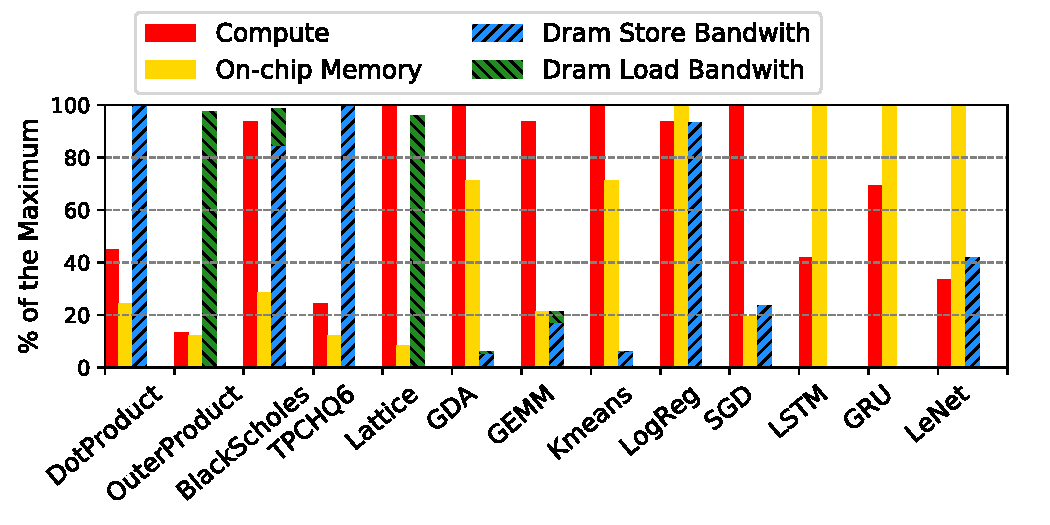
\includegraphics[width=0.8\columnwidth]{network/figs/util_bw2.pdf}
\caption[Resource and bandwidth utilization]{
  Physical resource and bandwidth utilization for various applications.}\label{fig:util_bw}
\centering
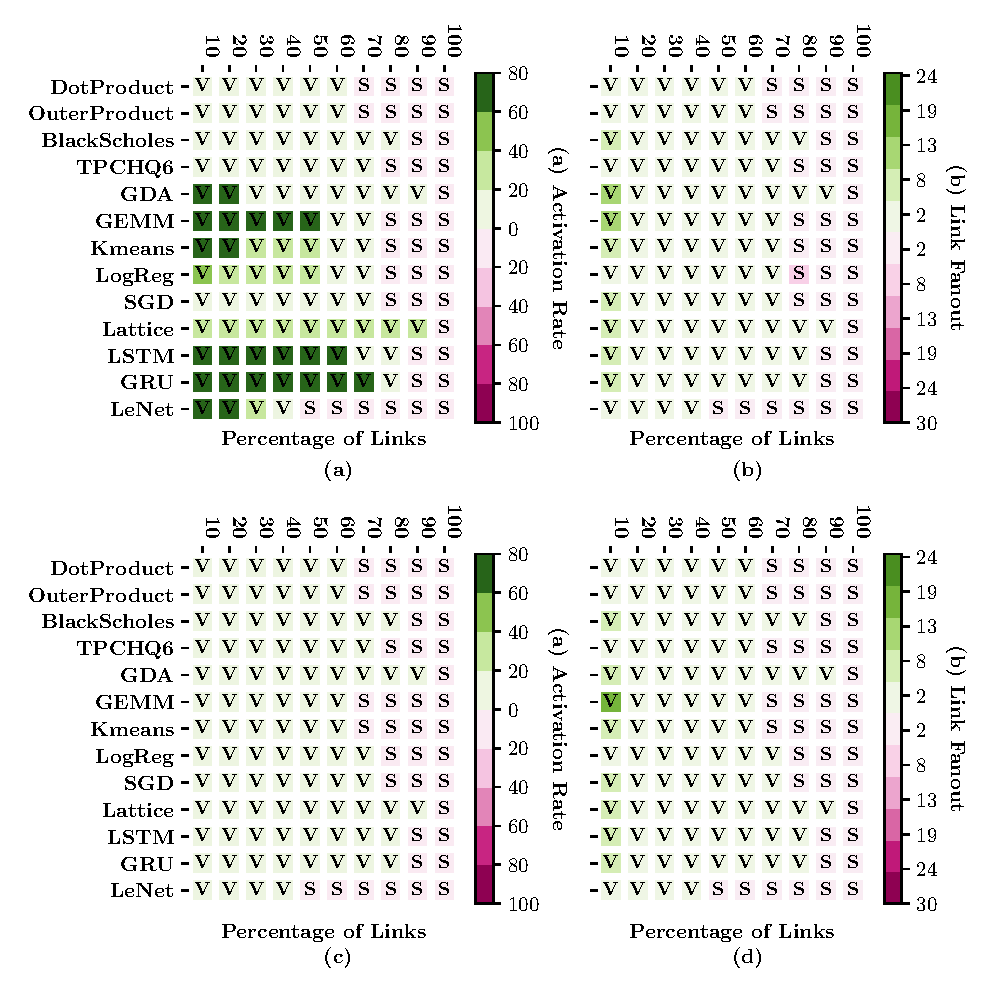
\includegraphics[width=0.8\columnwidth]{network/figs/link7.pdf}
  \caption[Application communication patterns]{Application communication patterns on pipelined (a,b) and scheduled (c,d) RDA architectures.
  (a) and (c) show the activation rate distribution of logical links at runtime. 
  Links sorted by granularity, then rate; darker boxes indicate higher rates.
  The split between green and pink shows the ratio of logical vector to scalar links. (b) and (d) show the distribution of broadcast link fanouts.
 }\label{fig:link}
\end{figure}

\begin{table*}
\centering
  \footnotesize
  \begin{tabular*}{6.25in}{p{0.75in} p{3in} p{2.5in}}
    \bottomrule
    \textbf{Benchmark} & \textbf{Description} & \textbf{Data Size} \\ \midrule
    DotProduct & Inner product & $1048576$ \\ \midrule
    OuterProduct & Outer product &$1024$ \\ \midrule
    BlackScholes & Option pricing &$1048576$ \\ \midrule
    TPCHQ6 & TPC-H query 6 &$1048576$ \\ \midrule
    Lattice & Lattice regression~\cite{garcia2009lattice} &$1048576$\\ \midrule
    GDA & Gaussian discriminant analysis &$127\times1024$ \\ \midrule
    GEMM & General matrix multiply &$256\times256\times256$ \\ \midrule
    Kmeans & K-means clustering &k=64, dim=64, n=8192, iter=2 \\ \midrule
    LogReg & Logistic regression &$8192\times128$, iter=4\\ \midrule
    SGD & Stochastic gradient descent for a single layer neural network &$16384\times64$, epoch=10 \\ \midrule
    LSTM & Long short term memory recurrent neural network &1 layer, 1024 hidden units, 10 time steps \\ \midrule
    GRU & Gated recurrent unit recurrent neural network &1 layer, 1024 hidden units, 10 time steps \\ \midrule
    LeNet & Convolutional neural network for character recognition& 1 image\\ \midrule
  \end{tabular*}
  \caption{Benchmark summary}
  \label{tab:benchmark}
\end{table*}

To study the communication patterns, 
we select a mix of applications from domains where hardware accelerators have shown promising performance and energy-efficiency benefits, such as linear algebra, databases, and machine learning.
Table~\ref{tab:benchmark} lists the applications and their data size.
Figure~\ref{fig:util_bw} shows, for each design, which resource limits performance: compute, on-chip memory, or DRAM bandwidth. 
DotProduct, TPCHQ6, OuterProduct, and BlackScholes are DRAM bandwidth-bound applications. 
These applications use few on-chip resources to achieve maximum performance, resulting in minimal communication.
Lattice (a fast inference model for low-dimensional regression~\cite{garcia2009lattice}), GDA, Kmeans, SGD, and LogReg are compute-intensive applications; for these, maximum performance requires using as much parallelization as possible. 
Finally, LSTM, GRU, and LeNet are applications that are limited by on-chip memory bandwidth or capacity. 
For compute- and memory-intensive applications, high utilization translates to a large interconnection network bandwidth requirement to sustain application throughput. 

Figure~\ref{fig:link}(a,b) shows the communication pattern of applications
characterized on the pipelined RDA architecture, including the variation in communication granularity. 
Compute and on-chip memory-bound applications show a significant amount of high-bandwidth communication (links with almost 100\% activity). 
A few of these high-bandwidth links also exhibit a high broadcast fanout. 
Therefore, a network architecture must provide sufficient bandwidth and efficient broadcasts to sustain program throughput.
On the contrary, time-scheduled architectures, shown in Figure~\ref{fig:link}(c,d), exhibit
lower bandwidth requirements due to the lower throughput of individual compute PUs. 
Even applications limited by on-chip resources have less than a 30\% firing rate on the busiest logical links; this reveals an opportunity for link sharing without sacrificing performance.

\begin{figure}
\centering
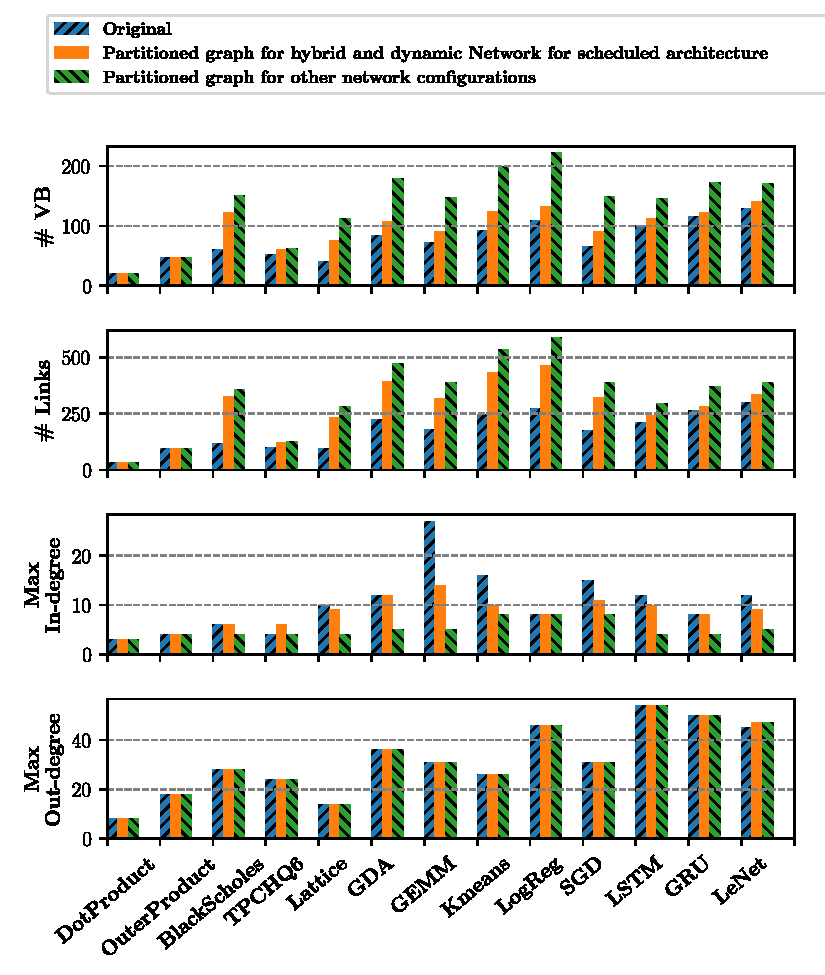
\includegraphics[width=0.9\columnwidth]{network/figs/graph.pdf}
\caption{Characteristics of program graphs.}\label{fig:graph}
\end{figure}

Figure~\ref{fig:graph} shows statistics describing the VU dataflow graph (VGDFG) before and after
the partitioning described in \Cref{sec:resalloc}. 
The blue bars show the number of VUs, number of logical links, and maximum VU input/output degrees in the original parallelized program; the yellow and green bars show the same statistics after partitioning. 
Fewer VUs are partitioned for hybrid networks and dynamic networks with the time-scheduled
architecture.
When a VU in a pipelined RDA consumes too many inputs or produces too many \emph{distinct} outputs,
\name partitions it to reduce its degree and meet the input/output bandwidth constraints of a purely static network. 
For dynamic and hybrid networks, partitioning is not strictly necessary, but it improves performance
by decreasing congestion at the network ejection port associated with a PU.
We do not partition broadcasts with high output degrees because they are handled natively within the network. 
Finally, the output degree does not change with partitioning because most outputs with a large degree are from broadcast links.

\subsection{Design Space for Network Architectures} \label{sec:networkds}

We start with several statically allocated network designs, where each SIMD pipeline connects to several switches, and vary flow control strategies and network bisection bandwidth.
In these designs, each switch output connects to exactly one switch input for the duration of the program.
We then explore a dynamic network, which sends program data as packets through an NoC.
The NoC uses a table-based routing scheme at each router to allow for arbitrary routes and tree-based broadcast routing.
Finally, we explore the benefits of specialization by evaluating design points that combine several of these networks to leverage the best features of each.

\subsubsection{Static networks}
We explore static network design points along three axes. 
First, we study the impact of flow-control schemes in static switches. 
In credit-based flow control~\cite{wang2013avoiding}, the source and destination PUs coordinate to ensure that the destination buffer does not overflow.
For this design point, switches only have a single register at each input, and there is no backpressure between switches.
The alternate design point uses a skid-buffered queue with two entries at each switch; using two entries enables per-hop backpressure and accounts for a one-cycle delay in stalling the upstream switch.
At full throughput, the receiver will consume data as it is sent and no queue will ever fill up.

The second axis studied is the bandwidth, and therefore routability, of the static network. 
We vary the number of connections between switches in each direction, which trades off area and energy for bandwidth.
Finally, we explore specializing static links: using a separate scalar network to improve routability at a low cost.

\subsubsection{Dynamic networks}
Our primary alternate design is a dynamic NoC using per-hop virtual channel flow control. 
Routing and Virtual Channel (VC) assignment are table-based: the compiler performs static routing and VC allocation, 
and results are loaded as a part of the routers' configurations at runtime.
The router has a separable, input-first VC and switch allocator with a single iteration and speculative switch allocation~\cite{dallytowles}.
Input buffers are sized just large enough (3 entries) to avoid credit stalls at full throughput.
Broadcasts are handled in the network with duplication occurring at the last router possible to minimize energy and congestion.
To respect the switch allocator's constraints, each router sends broadcasts to output ports sequentially and in a fixed order.
This is because the switch allocator can only grant one output port per input port in every cycle, and the RTL router's allocator does not have sufficient timing slack to add additional functionality.
We also explore different flit widths on the dynamic network, with a smaller bus taking multiple cycles to transmit a packet.

Because RDA networks are streaming---each PU pushes the result to the next PU(s) without explicit request---the network cannot handle routing schemes that may drop packets; otherwise, application data would be lost.
Because packet ordering corresponds directly to control flow, it is also imperative that all packets arrive in the order they were sent; this further eliminates adaptive or oblivious routing from consideration.
We limit our study of dynamic networks to statically placed and routed source routing due to these architectural constraints.
PUs propagate backpressure signals from their outputs to their inputs, so they must be considered as part of the network graph for deadlock purposes~\cite{hansson2007avoiding}.
Furthermore, each PU has fixed-size input buffers; these are far too small to perform high-throughput, end-to-end credit-based flow control in the dynamic network for the entire program \cite{wang2013avoiding}.
Practically, this means that no two logical paths may be allowed to conflict at \emph{any} point in the network; to meet this guarantee, VC allocation is performed to ensure that all logical paths traversing the same physical link are placed into separate buffers.

\subsubsection{Hybrid networks}
Finally, we explore hybrids between static and dynamic networks that run each network in parallel. 
During static place and route, the highest-bandwidth logical links from the program graph are mapped onto the static network; once the static network is full, further links are mapped to the dynamic network.
By using compiler knowledge to identify the relative importance of links---the link fanout and activation factor---hybrid networks can sustain the throughput requirement of most high-activation links while using the dynamic network for low-activation links.

\subsection{Performance, Area, and Energy Modeling} \label{sec:net_char}

Next section gives a quantitative analysis of the performance, area, and energy trade-offs involved 
in choosing a RDA network, using benchmarks showing in \Cref{tab:benchmark}.
This section outlines our methodology on how we capture the network performance, area, and energy in our evaluations.
\Cref{tab:notation} gives our notation for various network parameters discussed
in~\Cref{sec:networkds}.

\begin{table}
\footnotesize
  \centering
\begin{tabular*}{0.65\textwidth}{c l}
  \bottomrule
  \textbf{Notation} & \textbf{Description} \\\midrule
  $[$S,H,D$]$ & Static, hybrid, and dynamic network \\\midrule
  x<\#> & Static bandwidth on vector network (\#links between switches) \\\midrule
  %$s\#$ & Number of links between switches on static scalar network \\\midrule
  f<\#> & Flit width of a router or vector width of a switch \\\midrule
  v<\#> & Number of VC in router \\\midrule
  b<\#> & Number of buffers per VC in router \\\midrule
  $[$db,cd$]$ & Buffered vs. credit-based flow control in switch \\\midrule
  %$[Scheduled, Pipelined]$ & Time scheduled vs deep pipelined accelerator architectures \\\midrule
\end{tabular*}
\caption{Network design parameter summary.}
\label{tab:notation}
\end{table}

\subsubsection{Simulation}
We use a cycle-accurate simulator to model the pipeline and scheduling delay for the two types of architectures,
 integrated with DRAMSim \cite{dramsim} to model DRAM access latency. For static networks, we model
a distance-based delay for both credit-based and per-hop flow control. 
For dynamic networks, we integrate
our simulator with Booksim \cite{jiang2013detailed}, adding support for arbitrary source routing using look-up tables. 
Finally, to support efficient multi-casting in the dynamic network, we modify Booksim to duplicate broadcast packets at the router where their paths diverge.
At the divergence point, the router sends the same flit to multiple output ports over multiple cycles.
We assume each packet carries a unique ID that is used to look up the output port and next VC in a statically generated routing table, and that the ID is roughly the same size as an address.
When the packet size is greater than the flit size, the transmission of a single packet takes multiple cycles.

\subsubsection{Area and power}
To efficiently evaluate large networks, we start by characterizing the area and power consumption of individual routers and switches
used in various network configurations. 
The total area and energy are then aggregated over all switches and routers in a particular network.
We use router RTL from the Stanford open-source NoC router \cite{becker2012efficient} and our own parameterized switch implementation.
We synthesize using Synopsys Design Compiler with a \SI{28}{nm} technology library and clock-gating enabled, meeting timing at a 1 GHz clock frequency.
Finally, we use Synopsys PrimeTime to back-annotate RTL signal activity to the post-synthesis switch and router designs to estimate gate-level power.

We found that power consumption can be broken into two types: 
inactive power consumed when switches and routers are at zero-load ($P_{\text{inactive}}$, which includes both dynamic and static power),
and active power. The active power, as shown in Section~\ref{sec:net_char}, is proportional to the amount of
data transmitted. 
Because power scales linearly with the amount of data movement, we model the marginal energy to transmit a single flit of data (flit energy, $E_{\text{flit}}$) by dividing active energy by the number flits transmitted in the testbench:
\begin{equation}
  E_{\text{flit}} = \frac{\left(P-P_{\text{inactive}}\right) T_{\text{testbench}}}{\#\text{flit}} 
\end{equation}
While simulating an end-to-end application, we track the number of flits transmitted at each switch and router in the network, as well as the number of switches and routers allocated by place and route. 
We assume unallocated switches and routers are perfectly power-gated and do not consume energy.
The total network energy for an application on a given network ($E_{\text{net}}$) can be computed as:
\begin{equation}
  E_{\text{net}} = \sum_{\text{allocated}} P_{\text{inactive}} T_{\text{sim}}
  + E_{\text{flit}}  \#\text{flit},
\end{equation}
where $P_{\text{inactive}},$ $E_{\text{flit}},$ and $\#\text{flit}$ are tabulated separately for each network resource.

\begin{figure}
\centering
\includegraphics[width=0.8\columnwidth]{network/figs/sweep.pdf}
  \caption{Switch and router power with varying duty cycle.}\label{fig:sweep}
\end{figure}


Figure~\ref{fig:sweep} shows that switch and router power scale linearly with the rate of data transmission, but that there is non-zero power at zero-load. 
For simulation, the duty cycle refers to the amount of offered traffic, not accepted traffic.
Because our router uses a crossbar without speedup \cite{dallytowles}, the testbench saturates the router at 60\% duty cycle when providing uniform random traffic. 
Nonetheless, router power still scales linearly with accepted traffic.

A sweep of different switch and router parameters is shown in Figure~\ref{fig:char}. Subplots (d,e,f) show the energy necessary to transmit a single bit through a switch or router.
Subplot (a) shows the roughly quadratic scaling of switch area with the number of links between adjacent switches.
Vector switches scale worse with increasing bandwidth than scalar switches, mostly due to increased crossbar wire load. 
At the same granularity, a router consumes more energy a switch to transmit a single bit of data, even though the overall router consumes less power (as shown in Figure~\ref{fig:sweep}); 
this is because the switch has a higher throughput than the router.
The vector router has lower per-bit energy relative to the scalar router because it can amortize the cost of allocation logic, whereas the vector switch has higher per-bit energy relative to the scalar switch due to increased capacitance in the large crossbar. 
Increasing the number of VCs or buffer depth per VC also significantly increases router area and energy, but reducing the router flit width can significantly reduce the router area. 

\begin{figure}
\centering
\includegraphics[width=0.8\columnwidth]{network/figs/char.pdf}
  \caption{Area and per-bit energy for (a,d) switches and (b,c,f) routers. 
  The router only has a vector granularity and can be partially clock-gated when sending scalar packets.
  Subplots (f) show the energy of the vector router when used for scalar values (32-bit).}\label{fig:char}
\end{figure}

Overall, these results show that scaling static bandwidth is cheaper than scaling dynamic bandwidth, and a dynamic network with small routers can be used to improve link sharing for low bandwidth communication.  
We also see that a specialized scalar network, built with switches, adds a negligible area compared to and is more energy-efficient than the vector network. 
Therefore, we use a static scalar network with a bandwidth of 4 for the remainder of our evaluation, except when evaluating the pure dynamic network.
The dynamic network is also optimized for the rare instances when the static scalar network is insufficient. 
When routers transmit scalar data, the high bits of data buffers are clock-gated, reducing energy as shown in (f).
Figure~\ref{fig:area} summarizes the area breakdown of all the network configurations that we evaluate.

\begin{figure}
\centering
\includegraphics[width=1\columnwidth]{network/figs/area.pdf}
  \caption{Area breakdown for all network configurations.}\label{fig:area}
\end{figure}

\subsection{Network Architecture Evaluation} \label{sec:net_dse}

We evaluate our network configurations in five dimensions: performance (perf), performance per network area (perf/area), performance per network
power (perf/watt), network area efficiency (1/area), and network power efficiency (1/power). 
Among these metrics, performance is the most important: networks only consume a small fraction of the overall accelerator area and energy (roughly 10-20\%). 
Because the two key advantages of hardware accelerators are high throughput and low latency, 
we filter out a network design point if it introduces
more than 10\% performance overhead.
This is calculated by comparing to an ideal network with infinite bandwidth and zero latency.

For metrics that are calculated per application, such as performance, performance/watt, and power efficiency, we first normalize the metric with respect to the 
worst network configuration for that application. 
For each network configuration, we present a geometric mean normalized across all applications. 
For all of our experiments, except Section~\ref{sec:scale}, we use a network
size of $14\times14$ end-point PUs. All vector networks use a vectorization factor of 16 (\SI{512}{bit} messages).

\begin{figure}
\centering
\includegraphics[width=0.8\columnwidth]{network/figs/scale.pdf}
\caption{Performance scaling with increased RDA grid size for different networks.}\label{fig:scale}
\end{figure}
\subsubsection{Bandwidth scaling with network size}\label{sec:scale}
Figure~\ref{fig:scale} shows how different networks allow several applications to scale to different numbers of PUs.
For IO-bound applications (BlackScholes and TPCHQ6), performance does not scale with additional compute and on-chip memory resources.
However, the performance of compute-bound applications (GEMM and SGD) improves with increased resources, but plateaus at a level that is determined by on-chip network bandwidth. 
This creates a trade-off in accelerator design between highly vectorized compute PUs with a small network---which would be underutilized for non-vectorized problems---and smaller compute PUs with limited performance due to network overhead. 
For more finely grained compute PUs, both more switches and more costly (higher-radix) switches must be employed to meet application requirements.

The scaling of time-scheduled accelerators (bottom row) is much less dramatic than that of deeply pipelined architectures (top row). 
Although communication between PUs in these architectures is less frequent, the scheduled architecture must use additional parallelization to match the throughput of the pipelined architecture; this translates to larger network sizes. 

For pipelined architectures, both hybrid and static networks provide similar scaling with the same static bandwidth:
the additional bandwidth from the dynamic network in hybrid networks does not provide additional scaling. 
This is mostly due to a bandwidth bottleneck between a PU and its router, which prevents the PU from requesting multiple elements per cycle.
Hybrid networks tend to provide better scaling for time-scheduled architectures; multiple streams can be time-multiplexed at each ejection port without losing performance.

\subsubsection{Bandwidth and flow control in switches}

\begin{figure}
  \centering
\includegraphics[width=0.7\textwidth]{network/figs/radar_switch.pdf}
  \caption{
    Impact of bandwidth and flow control strategies in switches.}\label{fig:radar_switch}
\end{figure}

In this section, we study the impact of static network bandwidth and flow control mechanisms (per-hop vs. end-to-end credit-based). 
On the left side of Figure~\ref{fig:radar_switch}, we show that increased static bandwidth results in a linear performance increase and a superlinear increase in area and power. 
As shown in Section~\ref{sec:scale}, any increase in accelerator size must be coupled with increased network bandwidth to effectively scale performance. 
This indicates that network overhead will increase with the size of an accelerator.

The right side of Figure~\ref{fig:radar_switch} shows that, although credit-based flow control reduces the amount of buffering in switches and decreases network area and energy, application performance is significantly impacted. 
This is the result of imbalanced data-flow pipelines in the program: when there are parallel long and short paths over the network, there must be sufficient buffer space on the short path equal to the product of throughput and the difference in latency. 
Because performance is our most important metric, credit-based flow control is not feasible, especially because the impact of bubbles increases with communication distance, and therefore network size.

\subsubsection{VC count and reduced flit width in routers}
\begin{figure}
  \centering
\includegraphics[width=0.7\textwidth]{network/figs/radar_router.pdf}
  \caption{Impact of VC count and flit widths in routers.}\label{fig:radar_router}
\end{figure}
In this experiment, we study the area-energy-performance trade-off between routers with different VC counts. As shown
in Section~\ref{sec:net_char}, using many VCs increases both network area and energy.
However, using too few VCs may force roundabout routing on the dynamic network or result in VC allocation failure when the network is heavily utilized.
Nonetheless, the left side of Figure~\ref{fig:radar_router} shows minimal performance improvement from using more VCs. 

Therefore, for each network design, we use a VC count equal to the maximum number of VCs required to map all applications to that network. 
Figure~\ref{fig:vc} shows that the best hybrid network configurations with 2x and 3x static bandwidth require at most 2 VCs, whereas the pure dynamic network requires 4 VCs to map all applications.
Because dynamic network communication is infrequent, hybrid networks with fewer VCs provide both better energy and area efficiency than networks with more VCs, even though this constrains routing on the dynamic network.

\begin{figure}
\centering
\includegraphics[width=0.75\textwidth]{network/figs/vc.pdf}
  \caption{Number of VCs required for dynamic and hybrid networks. (No VCs indicates that all traffic is mapped to the static network.)}\label{fig:vc}
\end{figure}

We also explore the effects of reducing dynamic network bandwidth by using smaller routers;
as shown in Section~\ref{sec:net_char}, routers with smaller flits have a much smaller area.
Ideally, we could scale static network bandwidth while using a low-bandwidth router to provide an escape path and reduce overall area and energy overhead. 
The right side of Figure~\ref{fig:radar_router} shows that, for a hybrid network, reducing flit width improves area efficiency with minimal performance loss. 

\subsubsection{Static vs. hybrid vs. dynamic networks}

\begin{figure*}
\centering
\includegraphics[width=1\linewidth]{network/figs/perf.pdf}
  \caption{Normalized performance for different network configurations.}\label{fig:perf}
\end{figure*}

Figure~\ref{fig:perf} shows the normalized performance for each application running on several network configurations.
For some applications, the bar for S-x1 is missing; this indicates that place and route failed for all unrolling factors.
For DRAM-bound applications, the performance variation between different networks is trivial because only a small fraction of the network is being used. 
In a few cases (Kmeans and GDA), hybrid networks provide better performance due to slightly increased bandwidth.
For compute-bound applications, performance primarily correlates with network bandwidth because more bandwidth permits a higher parallelization factor. 

\begin{figure}
\centering
  \includegraphics[width=0.9\textwidth]{network/figs/energy.pdf} 
\caption{(a,d): Normalized performance/watt. (b,e): Percentage of compute and memory PUs utilized for each network configuration. 
  (c,f): Total data movement (hop count).}
\label{fig:energy}
\end{figure}

The highest bandwidth static network uses the most PUs, as shown in Figures~\ref{fig:energy}(b,e), because it permits more parallelization. 
It also has more data movement, as shown in (c,f), because PUs can be distributed farther apart. 
Due to bandwidth limitations, low-bandwidth networks perform best with small unrolling factors---they are unable to support the bisection bandwidth of larger program graphs.
This is evident in Figures~\ref{fig:energy}(b,e), where networks D-x0-v4-f512 and S-x2 have small PU utilizations.

With the same static bandwidth, most hybrid networks have better energy efficiency than the corresponding pure static networks, even though routers take more energy than switches to transmit the same amount of data.
This is a result of allowing a small amount of traffic to escape onto the dynamic network: with the dynamic network as a safety net, static PaR tends to converge to better placements with less overall communication.
This can be seen in Figures~\ref{fig:energy}(c,f), where most static networks have larger hop counts than the corresponding hybrid network; hop count is the sum of all runtime link traversals, normalized per-application to the network configuration with the most hops.
Subplots (e,f) show that more PUs are utilized with static networks than hybrid networks.
This is because the compiler imposes less stringent IO constraints on PUs when partitioning for the hybrid network (as explained in Section~\ref{sec:partition}), which results in fewer PUs, less data movement, and greater energy efficiency for hybrid networks.

\begin{figure}
  \centering
\includegraphics[width=0.7\textwidth]{network/figs/radar_best.pdf}
  \caption{Geometric mean improvement for the best network configurations, relative to the worst configuration.}\label{fig:radar_best}
\end{figure}
\begin{figure*}
\centering
\includegraphics[width=0.8\textwidth]{figs/pie.pdf}
\caption[Area and power breakdown of Plasticine]{
  Area and power breakdown of Plasticine using a static-dynamic hybrid network.
}
\label{fig:breakdown}
\end{figure*}

In Figure~\ref{fig:radar_best}, we summarize the best perf/watt and perf/area (among network configurations with <10\% performance overhead) for pipelined and scheduled RDA architectures. 
Pure dynamic networks are not shown because they perform poorly due to insufficient bandwidth.
On the pipelined RDA, the best hybrid network provides a 6.4x performance increase, 2.3x better energy efficiency, and a 6.9x perf/area increase over the worst network configuration. 
The best static network provides 7x better performance, 1.2x better energy efficiency, and 6.3x better perf/area. 
The hybrid network gives the best perf/area and perf/watt, with a small degradation in performance when compared to the static network. 
On the time-scheduled RDA, both static and hybrid networks have an 8.6x performance improvement. 
The hybrid network gives a higher perf/watt improvement at 2.2x, whereas the static network gives a higher perf/area improvement at 2.6x.
Overall, the hybrid networks deliver better energy efficiency with shorter routing distances by allowing an escape path on the dynamic network.

%\section{Plasticine Specialization for RNN Serving} \label{sec:rnn_arch}
To show efficient execution of the loop and parallel pattern constructs,
  we map our implementation onto a spatial architecture, Plasticine.
\textbf{Foreach} at Line $17, 19$ and \textbf{Reduce} at Line $22, 23$
  are mapped to PCUs on Plasticine.
When the application size is small,
  these constructs are executed using pipelined SIMD lanes within a single PCU.
When the application size is large,
  multiple PCUs can be used to parallelize and pipeline the dot
  product across PCUs. Element-wise operations can be executed in a deep pipeline
  formed by chaining multiple PCUs.

To fit an RNN's weights on-chip,
  we execute our application with low-precision arithmetics.
In this section,
  we propose the necessary micro-architectural changes to
  support low-precision arithmetics on Plasticine.
We also discuss architectural parameter selection for Plasticine
  to serve RNN applications efficiently.

\subsection{Mixed-Precision Support}
\label{sec:arch:varprec}
Previous works \cite{fowers2018configurable, jouppi2017datacenter}
  have shown that low-precision inference can deliver promising performance
  improvements without sacrificing accuracy.
In the context of reconfigurable architectures such as FPGAs,
  low-precision inference not only increases compute density,
  but also reduces required on-chip capacity for
  storing weights and intermediate data.

To support low-precision arithmetics without sacrificing coarse-grained reconfigurability,
we introduce two low-precision struct types in Spatial: a tuple of 4 8-bit and 2 16-bit floating-point 
numbers, \texttt{4-float8} and \texttt{2-float16} respectively.
Both types packs multiple low-precision values into a single precision storage.
We support only 8 and 16-bit precisions, which are commonly seen in deep learning inference hardwares.
Users can only access values that are 32-bit aligned.
This constraint guarantees that the microarchitectual change is only local to the PCU.
Banking and DRAM access granularity remains intact from the original design.

\begin{figure}
  \centering
  \includegraphics[width=1\columnwidth]{figs/lowprec.pdf}
  \caption{Plasticine PCU SIMD pipeline and low-precision support.
  Red circles are the new operations. Yellow circles are the original opertaions in Plasticine.
  In (d) the first stage is fused $1^{st}, 2^{nd}$ stages, and the second stage is fused
  $3^{nd}$, $4^{th}$ stages of (b).
   }
  \label{fig:lowprec}
  \vspace*{-0.3in}
\end{figure}
Figure \ref{fig:lowprec} (a) shows the original SIMD pipeline in a Plasticine PCU.
Each FU supports both floating-point and fix-point operations.
When mapping applications on Plasticine,
  the inner most loop body is vectorized across the lanes of the
SIMD pipeline, and different operations of the loop body are mapped to different stages.
Each pipeline stage contains a few pipeline registers (PRs)
  that allow propagation of live variables across stages.
%The PRs are accessible as both inputs and outputs of the FU.
%An FU can also read previous stage's PRs
%as its input value.
Special cross-lane connections as shown in red in Figure \ref{fig:lowprec} enable reduction operations.
To support 8-bit element-wise multiplication and 16-bit reduction, we add 4 opcodes to the FU, shown in
Figure \ref{fig:lowprec} (b).
The $1^{st}$ and $3^{rd}$ stages are element-wise, low-precision operations
  that multiply and add 4 8-bit and 2 16-bit values, respectively.
The $2^{nd}$ and $4^{th}$ stages rearrange low-precision values into two registers,
  and then pad them to higher precisions.
The $5^{th}$ stage reduces the two 32-bit value to a single 32-bit value using the existing add operation. 
From here, we can use the original
reduction network shown in Figure \ref{fig:lowprec} (a) to complete the remaining reduction and accumulates
in 32-bit connection.

With 4 lanes and 5 stages,
  a PCU first reads 16 8-bit values,
  performs 8-bit multiplication followed by rearrangement and padding,
  and then produce 16 16-bit values after the second stage.
The intermediate values are stored in 2 PRs per lane.
Next, 16 16-bit values are reduced to 8 16-bit values
  and then rearranged to 8 32-bit value in 2 PRs per lane.
Then, the element-wise addition in 32-bit value
  reduces the two registers in each line into 4 32-bit values.
These values are fed through the
  reduction network that completes the remaining
  reduction and accumulation in two plus one stages.

In a more aggressive specialization,
  we can fuse the multiply and rearange into the same stage.
We also fuse the first low-precision reduction with the next rearange as shown in Figure \ref{fig:lowprec} (d).
In this way, we can perform the entire low-precision map-reduce in 2 stages
  in addition to the original full precision reduction.
In order to maximize hardware reuse,
  we assume that it is possible to construct a full precision FU
  using low-precision FUs.
In addition, we observe that the original reduction network in the SIMD lanes
  could lead to low FU utilization.
To improve FU utilization, we fold the entire tree structure in a single stage.
Figure \ref{fig:lowprec} (c) shows the folded reduction accumulation structure.
Specifically, latter reductions in the tree are mapped to earlier stages in the pipeline.
In this setup, the entire reduction plus accumulation
  is still fully pipelined in $\log_2(\#_{LANE})+1$ cycles
  with no structural hazard.
With fused reduced-precision multiplication and reduction, and folded reduction tree,
  a PCU is able to perform all map-reduce that accumulates $4 \#_{LANE}$
  8-bit values using 4 stages.
All the operations are completed in $2+\log_2(\#_{LANE})+1$ cycles.

\subsection{Sizing Plasticine for RNN Serving}
Evaluating an RNN cell containing $N$ hidden units and $N$ input features
  requires $2N^2$ computations and $N^2+N$ memory reads.
With large $N$, the compute to memory ratio is 2:1.
The original Plasticine architecture uses a checkerboard layout
  with 1 to 1 ratio between PCU and PMU.
A PCU has 6 stages and 16 lanes, and a PMU has 16 banks.
This provides a 6:1 ratio between
  compute resource and on-chip memory read bandwidth.
As a result of this layout,
  on-chip memory read bandwidth becomes the bottleneck for accelerating RNN serving applications.
Given that RNNs cover a wide range of important applications,
  we select a Plasticine configuration tailored for RNN serving.
Specifically, we choose a 2 to 1 PMU-PCU ratio with 4 stages in each PCU.
Figure \ref{fig:arch} shows the layout of this Plasticine variant.
\begin{figure}
  \centering
  \includegraphics[width=\columnwidth]{figs/arch.pdf}
  \caption{Variant configuration of Plasticine for serving RNN.}
  \label{fig:arch}
  \vspace*{-0.2in}
\end{figure}

%\section{Generic Banknig Support (Ready)} \label{sec:banking_arch}

To support Spatial's generic banking scheme for on-chip SRAM mentioned in \Cref{sec:memsplit}, 
we need to introduce a few microarchitectural changes to Plasticine's datapath.
As a background, the static banking analysis searches an address remapping scheme, which we refer as
banking scheme, that remaps the logical address space into partitions, such that addresses accessed
in parallel belongs to different partitions. 
Each partition corresponds to a physical memory bank that comes with an additional address port.
If the compiler can find a way to partition the data such that all parallel workers are sent to
different physical banks, the memory is guaranteed to feed all workers at full-throughput, which
scales performance with parallelism.
To search for the banking schemes, the compiler analyzes the access patterns of the memory.
An access pattern refers to groups of address expressions that can be queried concurrently.
For each access pattern, there can be multiple banking schemes that can sustain the access bandwidth.
However, not all schemes cost the same amount of resources; some are more expensive in logic, and
others are more expensive in memory.

The partitioning logic are two parametrizable equations for the bank address (BA) and the bank offset (BO),
both are functions of the original user-requested logical addresses.
BA is an expression that selects the partition for each request, and BO is the offset within the partition.
The banking analyzer searches the parameters in the equation and injects these computations to
memory accesses in the program. 
The first addition to Plasticine is the ability to compute independent BI and BO for each vector
lanes. 
We introduce vectorized address pipelines in PMUs, which was originally a scalar pipeline.

The generic banking scheme also requires a full crossbar datapath between all access lanes (workers) and
physical banks. To support this, we introduce the shuffle operator shown in \Cref{fig:memsplit}.
The shuffle operator takes three vectorized operands: a from address $\overrightarrow{FA}$, a to address
$\overrightarrow{TA}$, and a base $\overrightarrow{B}$.
The output $O$ equals to $B$ shuffled from the order specified in $\overrightarrow{FA}$ to the order in
$\overrightarrow{BA}$. 
Specifically,
\begin{align}
\forall i \in [1,|\overrightarrow{O}|],
O_i &= \begin{cases}
B_j, \text{if $\exists$ $TA_i = FA_j$}\\
0
\end{cases} \\
|\overrightarrow{FA}| &= |\overrightarrow{B}| \\
|\overrightarrow{TA}| &= |\overrightarrow{O}|
\end{align}
\Cref{fig:memsplit} gives concrete examples of inputs and outputs of the shuffle operator.
On the requester side, $BA$ is the $FA$, a vector constant corresponding to the banks statically
assigned to the partition is the $TA$, and $BO$ is the base.
On the receiver side, the vector constant is the $FA$, the $BA$ is the $TA$, and the data response
$D$ is the base.
If a lane in the $TA$ is not in the $FA$, the corresponding lane is marked as invalid with value
$0$. As a result, an invalid vector ORed with a valid vector is still the valid vector.
For address going to the scratchpad, we use the first bit of the 32-bit address as the predication
bit of the access; if the predicate bit equals zero, the request will be dropped by the memory.
Therefore, a valid address zero would be xF0000000 to distinguish with an invalid address 0.

The shuffle operator can be expensive, requiring a $16\times16$ 32-bit crossbar with parallel
integer comparators for equality. We expect to add one or two shuffle operators per SIMD pipeline,
and the operator can be pipelined across multiple stages to meet timing.



%\chapter{Related Work} \label{sec:related}

\section{Compiler}
\paragraph{Streaming Dataflow IRs}
Although many works claim to emit efficient and information-rich dataflow IRs for the downstream compilers, 
very few of them can capture the high-level parallel patterns and implementation details that are critical 
to RDA mappings. 
For example, TensorFlow \cite{tensorflow} emits dataflow IR composed of tensor operations. 
However, its IR lacks information on the parallel patterns within these operations. 
In contrast, most of 
the streaming languages \cite{streamit, synaid, maxj} are not able to extract nested loop-level parallelism 
from modern data-intensive applications. 
For example, StreamIt \cite{streamit}, a language tailored for streaming computing, also adopts distributed 
control as in \name{}. 
However, it lacks the necessary language features to describe deeply and irregularly nested loops that are 
common in modern data-intensive applications.

%\paragraph{Hardware Architectures}
%Spatial reconfigurable accelerators (\eg, Dyser~\cite{dyser} and Tartan~\cite{tartan}) have only one-level of hierarchy.
%Hence, such accelerators' performance can be bottlenecked by their limited interconnect bandwidth and power budget.
%Sparse Processing Unit (SPU)~\cite{sparseaccel} can sustain higher interconnect bandwidth by introducing on-chip hierarchy; however, it lacks support for polyhedral memory banking~\cite{poly_cong}, a pivotal optimization to achieve massive parallel accesses to on-chip memory. Plasticine~\cite{plasticine} provides us with the desired architecture features; however, its compiler lacks the necessary components to support efficient streaming execution. Given that Plasticine resembles many key features of the RDA model, we target Plasticine with \name{}.

\paragraph{Machine Learning Compilers}
\begin{outline}
\1 TensorFlow
\1 Theano: A Python framework for fast computation of mathematical expressions.
\1 Cognitive computing programming paradigm: a corelet language for composing networks of neurosynaptic
cores. I
\cite{onnc}
\end{outline}

Library approach
\begin{outline}
\1 Mxnet: A flexible and efficient machine learning library for heterogeneous distributed systems
\1 Anintroductiontocomputational networks and the computational network toolkit
\1 Neural Network Transformation and Co-design under Neuromorphic Hardware Constraints.
\1 Caffe: Convolu- tional architecture for fast feature embedding.
\1 Cambricon: An instruction set architecture for neu- ral networks.
\1 Tangram: Optimized Coarse-Grained Dataflow for Scalable NN Accelerators
\end{outline}

Kernel-specific loop optimization
\begin{outline}
\1 Tangram: Optimized Coarse-Grained Dataflow for Scalable NN Accelerators
\end{outline}

\paragraph{ML Accelerators}
\begin{outline}
%% Dataflow accelerators
\1 A runtime reconfigurable dataflow processor for vision
\1 Tangram: Optimized Coarse-Grained Dataflow for Scalable NN Accelerators
\1 %% domain specific loop fushion inter change
\1 Truenorth: Design and tool flow of a 65 mw 1 million neuron programmable neurosynaptic chip. from
IBM
\1 Memristive Boltzmann machine: A hardware accelerator for combinatorial optimization and deep
learning. 
\1 Scalable hierarchical network-on- chip architecture for spiking neural network hardware
implementations. 
\1 Diannao: A small-footprint high-throughput accel- erator for ubiquitous machine-learning.
\1 Pudiannao: A polyvalent machine learning accelerator. In ACM SIGARCH Computer Architecture News, Vol.
43. ACM, 369–381.
\1 Eyeriss: An energy- efficient reconfigurable accelerator for deep convolutional neural networks. I
\1 EIE: efficient inference engine on compressed deep neural network.
\1 Design and evolution of modular neural network architectures
\1 In-Datacenter Performance Analysis of a Tensor Processing Unit. 
\1 RENO: A high- efficient reconfigurable neuromorphic computing accelerator design.
\1 Convolution engine: balancing efficiency \& flexibility in specialized computing.
\1 Minerva: Enabling low-power, highly-accurate deep neural network acceler- ators. 
\1 DNPU: An 8.1TOPS/W Reconfigurable CNN-RNN Processor for General Purpose Deep Neu- ral Networks. 
\1 C-Brain: A deep learning accelerator that tames the diversity of CNNs through adaptive data-level
\1 parallelization. 
\end{outline}

\paragraph{Spatial Compilers}
Most previous works \cite{nowatzki, spatial-computation} only consider allocating resources at the same level. 
\name{} takes a more general assumption by co-allocating resources at multiple levels of an accelerator's hierarchy.

%The Plasticine compiler~\cite{plasticine} is similar to \name{} that it also uses a token-based control protocol.
%However, it performs worse than \name{} due to the following reasons.
%First, the Plasticine compiler allocates VBs for every level of Spatial's (a high-level language) control hierarchy. 
%The communication between parent and child controllers lead to both communication hotspots around the parent, and bubbles before entering a steady-state of the loop iterations. 
%Second, the Plasticine compiler assigns a single memory PB for each logical memory in the Spatial program. 
%Hence, it could not handle the case where a logical memory exceeds the capacity or bank limits of the physical PBs.
%Third, the Plasticine compiler only supports polyhedral memory partitioning at the first dimension of the on-chip memory. 
%Hence, its applicability to data-intensive applications with high-dimension tensor algebra is questionable.
%Last, compared to \name{}'s separate allocation and assignment phases described in
%\Cref{sec:control} and \Cref{sec:resalloc},
%the Plasticine compiler allocates one VB for a specific type of PB and underutilizes resources within PBs.

\section{On-Chip Network}

Multiple decades of research have resulted in a rich body of literature, both in CGRAs~\cite{cgraSurvey1, cgraSurvey2} and on-chip networks~\cite{ocn-synthesis}. We discuss relevant prior work under the following categories:
\subsection{Tiled Processor Interconnects} Architectures such as Raw~\cite{raw} and Tile~\cite{tile} use scalar operand networks~\cite{son}, which combine static and dynamic networks. Raw has one static and two dynamic interconnects: the static interconnect is used to route normal operand traffic, one dynamic network is used to route runtime-dependent values which could not be routed on the static network, and the second dynamic network is used for cache misses and other exceptions. Deadlock avoidance is guaranteed only in the second dynamic network, which is used to recover from deadlocks in the first dynamic network. However, as described in Section~\ref{sec:intro}, wider buses and larger flit sizes create scalability issues with two dynamic networks, including higher area and power. In addition, our static VC allocation scheme ensures deadlock freedom in our single dynamic network, obviating the need for deadlock recovery.
The dynamic Raw network also does not preserve operand ordering, requiring an operand reordering mechanism at every tile.

TRIPS~\cite{trips} is a tiled dataflow architecture with dynamic execution. TRIPS does not have a static interconnect, but contains two dynamic networks~\cite{trips-network}: an operand network  to route operands between tiles, and an on-chip network  to communicate with cache banks. Wavescalar~\cite{wavescalar} is another tiled dataflow architecture with four levels of hierarchy, connected by dynamic interconnects that vary in topology and bandwidth at each level. The Polymorphic Pipeline Array~\cite{ppa} is a tiled architecture built to target mobile multimedia applications. While compute resources are either statically or dynamically provisioned via hardware virtualization support, communication uses a dynamic scalar operand network.

\subsection{CGRA Interconnects}
Many previously proposed CGRAs use a word-level static interconnect, which has better compute density than bit-based routing~\cite{bus-fpga}. CGRAs such as HRL~\cite{hrl}, DySER~\cite{dyser}, and Elastic CGRAs~\cite{elasticCGRAs} commonly employ two static interconnects: a word-level interconnect to route data and a bit-level interconnect to route control signals.
Several works have also proposed a statically scheduled interconnect~\cite{van2009static, dimitroulakos2006exploring, wave} using a modulo schedule. While this approach is effective for inner loops with predictable latencies and fixed initiation intervals, variable latency operations and hierarchical loop nests add scheduling complexity that prevents a single modulo schedule. HyCube~\cite{hycube} has a similar statically scheduled network, with the ability to bypass intermediate switches in the same cycle. This allows operands to travel multiple hops in a single cycle, but creates long wires and combinational paths and adversely affects the clock period and scalability.
%However, applications with a hierarchical nesting of loops provide two poor options to arrive a single modulo schedule: the II can be extended to cover the entirety of the innermost loop, or the outer loop can have resources reserved in the inner loop schedule.
%The first option is frequently not realistic because scheduled hardware has a hard cap on the II, and loops can be of arbitrary length.
%If outer loops have resources reserved in the inner loop schedule, then the schedule will become congested with reserved, but infrequently used, resources.
\subsection{Design Space Studies} Several prior studies focus on tradeoffs with various network topologies, but do not characterize or quantify the role of dynamism in interconnects.
The Raw design space study~\cite{dse-raw} uses an analytical model for applications as well as architectural resources to perform a sensitivity analysis of compute and memory resources focused on area, power, and performance, without varying the interconnect. The ADRES design space study~\cite{dse-adres} focuses on area and energy tradeoffs with different network topologies with the ADRES~\cite{adres} architecture, where all topologies use a fully static interconnect. KressArray Xplorer~\cite{dse-kressarray} similarly explores topology tradeoffs with the KressArray~\cite{kress} architecture. Other studies explore topologies for mesh-based CGRAs~\cite{dse-date} and more general CGRAs supporting resource sharing~\cite{dse-tvlsi}. Other tools like Sunmap~\cite{sunmap} allow end users to construct and explore various topologies.

\subsection{Compiler Driven NoCs (WIP)}
Other prior works have used compiler techniques to optimize various facets of NoCs.
Some studies have explored statically allocating virtual channels~\cite{staticVC-isca, staticVC-nocs} to multiple concurrent flows to mitigate head-of-line blocking. These studies propose an approach to derive deadlock-free allocations based on the turn model~\cite{turnModel}. While our approach also statically allocates VCs, our method to guarantee deadlock freedom differs from the aforementioned study as it does not rely on the turn model.
Ozturk et al. \cite{ozturk2010compiler} propose a scheme to increase the reliability of NoCs for chip multiprocessors by sending packets over multiple links.
Their approach uses integer linear programming to balance the total number of links activated (an energy-based metric) against the amount of packet duplication (reliability).
Ababei et al. \cite{ababei2011energy} use a static placement algorithm and an estimate of reliability to attempt to guide placement decisions for NoCs.
Kapre et al. \cite{kapre2011noc} develop a workflow to map applications to CGRAs using several transformations, including efficient multicast routing and node splitting, but do not consider optimizations such as non-minimal routing.

%Our approach provides an extension of these techniques by using a ``closed-loop'' iterative process.
%Instead of doing each step (placement, routing, deadlock avoidance) sequentially, we are able to use heuristics to quantify the impact that each step has on the badness of the overall design.
%For example, this allows us to fix routing pathologies by re-placement, because we can identify the specific placement decisions that led to the poor set of routes.


% Ignore arch for now; we assume arch

% \paragraph{Plasticine Compiler}
% The Plasticine compiler described in the original paper also uses a token-based control protocal.
% However, the Plasticine compiler still allocates VB for each level of the controller hierarchy in Spatial
% and pass tokens between the parent and child controllers, which creates communication hot-spot around the
% parant controller and suffers from bubble during warmup phase of the loop iteartions.
% \yz{Rephrase this}
% In addition, their compiler assigns a single memory PB to each logical memory in the program; 
% the compiler cannot handle logical memory exceeding capacity or bank limit of the physical PBs.
% The simple strided banking scheme also disallows parallelized access on multiple dimension of the memory,
% which can greatly limits the application design space.
% Finally, unlike spaerate allocation and assignment phases described in \Cref{sec:alloc} and \Cref{sec:pruning},
% they allocate a VB for a specific type of PB, which under under utilizes resource whin PBs.


% \gist{
% CGRA: \\
% \cite{tartan} \\
% Imperative to Spatial Architectures: \\
% \cite{synaid}: 
% \begin{outline}
% \1 Target green array. Tiles of stack based 18-bit processors. Small local memory per
% core.
% \1 Small benchmarks: trigonometric, FFT, bithack, etc..
% \end{outline}
% \cite{zaidi}
% His thesis:\\
% \url{https://www.cl.cam.ac.uk/techreports/UCAM-CL-TR-870.pdf} \\
% Targeting FPGA. We probably don't want to cite this guy.

% Partitioning: \\
% \cite{nowatzki} - Partitioning data flow graph using ISL \\

% Summary:
% Looks like we are not the first one trying to map imperative language to spatial architecture. But there are still major differences.
% Some of the work is mapping to FPGAs, similar to high-level synthesis tools.
% Many of the other works like \cite{zaidi} only focus on the data-flow graph and do not handle memory accesses. Although we both trying to support imperative language on spatial accelerator, our focus is never to accelerate control heavy code on the accelerator, but rather to target data intensive application with more flexibility.

% \cite{synaid} is actually very relevant but the architecture is at a much smaller scale. It does have distributed on-chip memory but their memory is a stack used to store program for processors. None of the prior work has consider using distributed memory to compose logically single memory with strong-consistency and coherence. Another major difference is that these architecture does not have global network and DRAM that introduces variable latency. 
% So this changes how the application is mapped onto the accelerator. Our approach is completely distributed streaming approach while they tends to use statically scheduled approach.
% Finally the applications are very different. Most of their applications are very small kernels or image/audio encoding/decoding. Our benchmarks has a mix of full ML models + graph + others
% }

% Maybe related \cite{sparseaccel}

% Triggered Instruction \cite{ti}
% Tartan\cite{tartan}

% \gist{
% 	\begin{itemize}
% 		\item Plasticine compiler: \cite{plasticine}
% 		\item Tartan: \cite{tartan} Single op partitions w/ handshaking, direct template translation.
% 		\item Zaidi Thesis: \cite{zaidi} Conversion to bluespec, also uses token-based control. No partitioning / merging.
% 		\item Partitioning: \cite{nowatzki} Solver-based partitioning, very small arrays (4x4 dyser, etc.), with statically known delays and single-op partitions. Does not handle merging.
% 		\item SparseAccel: \cite{sparseaccel}\ Architecture paper, basically nothing about compilers.  (NR)
% 		\item streamit for RAW: \cite{streamit} No memory consistency due to pure stream structure, fine grained arch. Mesh of processors.
% 		\item Triggered Instructions \cite{ti} Fine grained processor architecture, with caches. (Micro paper: manual mapping, assembly, NR)
% 		\item Chlorophyll: \cite{synaid} Maps subset of C to GreenArrays (small spatial stack-processor architecture). Distinct Non-distributed arrays vs distributed arrays, optional partition annotations, static for loops (unrestricted while), uses Rosette backend solver (branch and bound, SA, Ant, Tabu Search, picked Simulated Annealing). Actual generation is synthesis based.
% 		\item Spatial computation \cite{spatial-computation} Maps ANSI C to Verilog, handshake + token based execution with speculative execution. Uses crossbar network for memory (although we assume pre-banked memory). Fine grained control, uses Pegasus for memory dependence graph and tokens for synchronization. Does not address partitioning / merging.
% 	\end{itemize}
% }

%%\chapter{Future Work (WIP)}


%\chapter{Conclusions (WIP)} \label{sec:conclusion}

Reconfigurable dataflow accelerators (RDAs) are a promising class of spatial accelerators, which deliver higher performance-to-resource efficiency than conventional process architectures while capturing a large application space.
However, to sustain these benefits as RDAs get larger, the software stack must address the challenges of (a) distributed control / correctness and (b) efficient resource allocation.

We address these challenges by proposing a distributed asynchronous control scheme and a program decomposition method. 
We develop a compiler, \name{}, that constructs a virtual block dataflow graph (VBDFG) from a program specification and generates a minimal set of peer-to-peer synchronizations, which allow fine-grained parallelization factors that would otherwise incur large communication overheads.
Furthermore, operations on VBDFG are decomposed and assigned to a heterogenous collections of physical blocks (PBs). 
Lastly, we implement these techniques and through evaluations show that \name{} achieves a speedup of 4x over a Tesla V100 GPU.
We hope that the approach and implementation presented in this work will help scale modern RDAs add a steady pace..

We show that the best network design depends on both applications and the underlying accelerator architecture.
Network performance correlates strongly with bandwidth for streaming accelerators, and scaling raw bandwidth is more area- and energy-efficient with a static network.
We show that the application mapping can be optimized to move less data by using a dynamic network as a fallback from a high-bandwidth static network.
%this contributes a 6.9x average performance per area and 2.3x average energy-efficiency improvement for a static-dynamic hybrid network.
This static-dynamic hybrid network provides a 1.8x energy-efficiency and
2.8x performance advantage over the purely static and purely dynamic networks, respectively.
  %Furthermore, we show that spatial architectures require larger switches as programs get bigger, imposing super-linear scaling of network size with chip area.




% now for the body of the thesis, modify the number of these lines as needed

% this includes chapter1.tex which should start with a \chapter{...}
% command 

% and the end material

\appendix

\chapter{Appendix}

\section{Context Programming Restrictino}

We use the imperative context configuration for ease of understanding, but it is important to
realize not all program expressible at this abstraction can be executed by the PCU.

\begin{figure}
  \begin{subfigure}[b]{0.5\textwidth}
    \inputminted{python}{code/dotproduct.py}
    \caption{Declarative configuration}
  \end{subfigure}
  \hfill
  \begin{subfigure}[b]{0.4\textwidth}
    \inputminted{python}{code/context_imp.py}
    \caption{Imperative configuration}
  \end{subfigure}
  %\caption[Example PCU configuration]{
  %}
  %\label{fig:context}
\end{figure}


% bibliography.tex should include either 
% \bibliographystyle{...}
% \bibliography{mythesis}
% or some other way of doing the bibliography
\bibliographystyle{ieeetr}
\bibliography{text/references}

\end{document}

